\chapter{Receiver design and development}\label{chap:instrumentation}

% **************************** Define Graphics Path **************************
\ifpdf
    \graphicspath{{instrumentation/figs/Raster/}{instrumentation/figs/PDF/}{instrumentation/figs/}}
\else
    \graphicspath{{instrumentation/figs/Vector/}{instrumentation/figs/}}
\fi

Measurements of the radio-sky require an instrument called a ‘radiometer’, a machine that measures incoming radiation. A radiometer usually consists of two main components; an antenna to collect an electromagnetic waves and a device to measure the signal's power such as a spectrometer. As more advanced instruments are deployed, additional processes are implemented to condition this information before being sent to the spectrometer such as amplification of weak signals and filtering to an frequencies of interest such that a new intermediary device is often introduced as a bridge between the antenna and the spectrometer known as a ‘receiver’.

The addition of components such as a receiver will necessarily produce more complicated forms of systematic noise, through things like reflections spawned from impedance mismatches at connections which hamper the detection and analysis of astrophysical phenomena. Characterising the interaction of the various instrument components as well as the resulting noise is undertaken through auxiliary devices which inform the process of ‘calibration’ in order to ultimately remove systematics and facilitate detection of cosmic signals. Consideration for the ensemble of devices, their control and monitoring is a principle area of experimental instrument design and the development of new architecture and engineering techniques to accommodate the unique requirements of individual experiments is the focus of this next chapter.


% =========================================
\section{The REACH receiver}\label{sec:receiver_general}
The REACH receiver is designed to address concerns brought forth with other experiments regarding residual systematics in their data while permitting the innovative features of the overall radiometer. Primarily, the broad bandwidth used by REACH makes it impractical to develop an achromatic antenna that provides a perfect impedance match between the antenna and receiver. Reflections spawned from this contact point result in considerable spectral variation across the observational band on the order of tens of Kelvin due to the overwhelming synchrotron foreground at these frequencies. Furthermore, while the method of ‘relative calibration’ was historically used to characterise narrow-band instruments, wide-band radiometers must obtain an absolute flux scale in frequency to measure the frequency-dependent sky-averaged brightness temperature through ‘absolute calibration’, which necessitates a series of additional components and switches.

Another primary focus of the design approach was the ability to calibrate the instrument completely in the field\footnote{While this philosophy was not completely adhered to in the final deployed system, the spirit of this ambition guided the entire receiver development. Please see CHAPTER ON S-PARAMETER CORRECTIONS for more details.} as opposed to previous experiments where the devices were characterised in controlled laboratory settings before deployment. The environmental (e.g. temperature and humidity) dependence of the sensitive electronic components provided a challenge to be addressed in the receiver design which requires system and temperature stability in the field as well as full autonomy.

In response to these considerations, the REACH receiver system is comprised of two subsystems, the receiver ‘front-end’ that sits under the raised antenna ground plane and the receiver ‘back-end’, also known as the readout system, which is separated from the front-end by a 100 metre distance connected by a Radio Frequency over Fibre (RFoF) link and powered by solar panels. A conceptual diagram of the radiometer system is shown in \cref{fig:system_diagram}. Many of the environment-sensitive components responsible for calibration and conditioning of the data are included in the front-end, with the back-end containing components for spectral data collection, control and signal processing as detailed below.
\begin{figure}
    \centering
    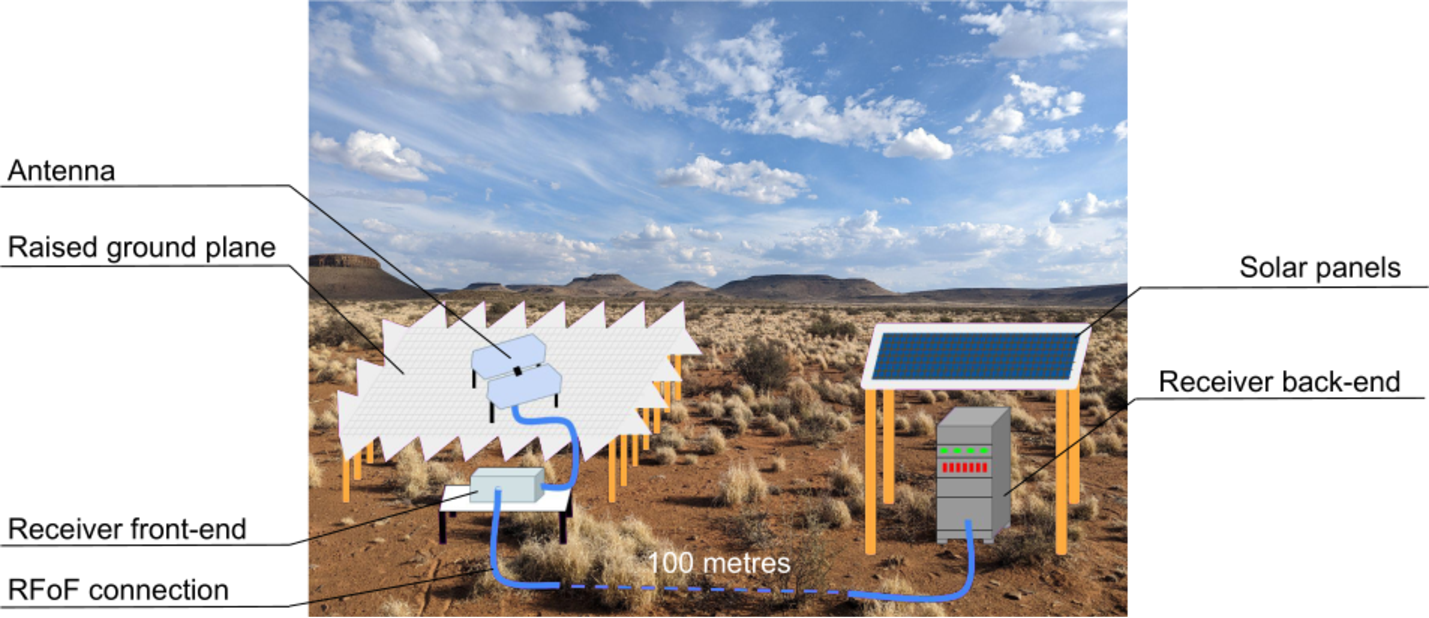
\includegraphics[width=\textwidth]{system_diagram}
    \caption{An illustration of the REACH radiometric system showing the hexagonal dipole antenna on a raised ground plane above the receiver front-end linked to the back-end and solar panels by 100 metres of fibre optic cable. The background image is a picture taken of the REACH deployment site located in the South African Karoo Radio Astronomy Reserve.}
    \label{fig:system_diagram}
\end{figure}


% =========================================
\subsection{Receiver front-end}\label{sec:frontend}
The front-end contains the most sensitive radiometer components housed in a sealed enclosure to facilitate calibration of the instrument to the highest accuracy. As the maintenance of environmental stability is difficult to achieve over long periods of time in the field, the project’s emphasis on an in situ calibration could only be achieved through a conscious effort to minimise the volume of the receiver front-end such that a constant temperature is kept via thermal devices while drawing a sustainable amount of power from the solar panels which are rated to give a maximum of 135 W of power to the front-end. Given this as a primary focus during the design process, nearly all of the components in the front-end were chosen based on a careful balance between their compact size and superior quality.


% =========================================
\subsubsection{The front-end enclosure}
The entirety of the receiver front-end is contained in a $500 \times 500 \times 210$ mm Rittal AE 1007.600 stainless steel enclosure serving as an RF-shield with category IP 66 protection against dust and water from the outside environment. 20 mm\footnote{18 mm in actuality when measured} of Kingspan Kooltherm K5 External Wall Insulation Board lines the inner walls of the enclosure in order to assist with temperature stability. Original designs used 11 mm Zotefoam for its efficient absorption of infrared radiation as used by the BICEP and Keck Array, but thermal tests showed this material to be less efficient during cooling compared to the 0.021 Wm\textsuperscript{-1}K\textsuperscript{-1} thermal conductivity of the building-standard Kooltherm sheets. Six connection ports were drilled into the enclosure to interface with external components; one for connection to the antenna sitting directly above the receiver on the raised ground plane via 150 mm Heliax cable, two for control and monitoring via USB over fibre-optical link, one RFoF connection for communication with the receiver back-end, one SubMiniature version-A (SMA) port for the 48 V DC power supply from the solar panels and an additional coaxial SMA port for testing and triage in the field. EMI gaskets were placed around the openings to reduce the impact of self-generated RFI towards the antenna as well as external RFI from feeding into the signal chain. A diagram of the enclosure’s external connections is shown in \cref{fig:enclosure_external_connections}.
\begin{figure}
    \centering
    \includegraphics[width=\textwidth]{enclosure_external_connections}
    \caption{The external connections of the receiver front-end enclosure showing the coaxial antenna connections, USB to fibre connections in blue, RFoF connection in green, power connection and additional port for in-field diagnostics and testing. The orientation shown is the same as during deployment.}
\label{fig:enclosure_external_connections}
\end{figure}

The metal framing of the enclosure also served as a heat dump for the encased electrical components using a custom heat exchanger and fan-assisted heat sink as detailed in the next section. To assist with the thermal considerations, the receiver front-end components are mounted on a 3 mm baseplate as shown in \cref{fig:enclosure_plate} to allow airflow between the plate and the internal heat exchanger.
\begin{figure}
    \centering
    \begin{minipage}{.4\textwidth}
        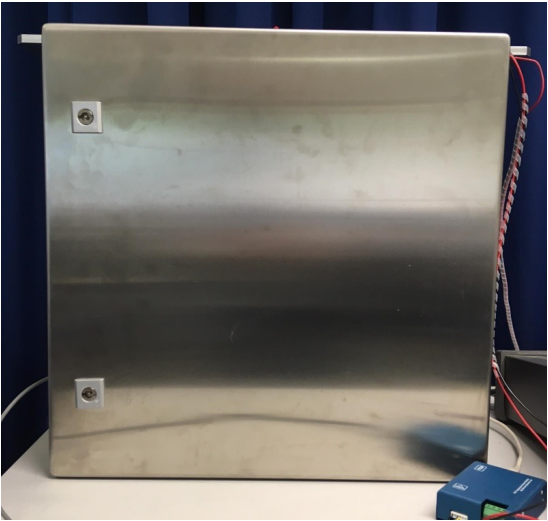
\includegraphics[scale=0.55]{enclosure}
        \vfill
        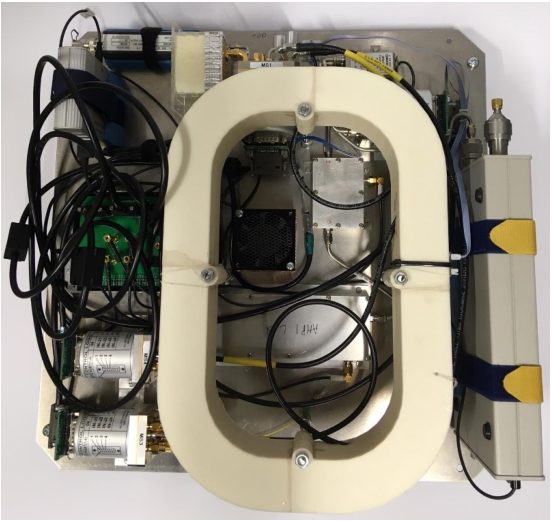
\includegraphics[scale=0.55]{component_plate}
    \end{minipage}
    \begin{minipage}{.4\textwidth}
        \centering
        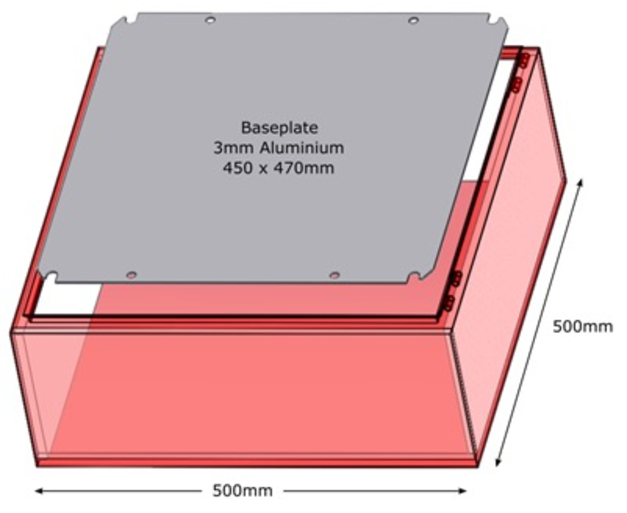
\includegraphics[scale=0.57]{enclosure_plate}
    \end{minipage}
    \caption{A picture of the front-end enclosure is shown on the top left. The bottom left shows the front-end components bolted onto the 3 mm baseplate. The diagram on the right depicts the baseplate's insertion into the enclosure.}
    \label{fig:enclosure_plate}
\end{figure}


% =========================================
\subsubsection{Front-end thermal management system}
Front-end temperature stability is maintained through a stack of components placed below the centre of the baseplate. A 113 watt Laird UltraTEC UT6-24-F1-5555 proportional integral derivative thermoelectric cooler (TEC) drives cooling or heating through the Peltier effect which is coupled to the receiver component baseplate by a $55 \times 55 \times 16$ mm copper stack. A thermal gap pad connects the bottom of the TEC module with a larger copper plate on the enclosure wall allowing heat transfer to an external Fischer LA7 150-1 heatsink and fan for expulsion of heat to the outside environment.

An initial test of this setup was conducted by placing a 40 W $110 \times 110$ mm heating source below the receiver component baseplate centre which recorded a 5 K (or 8 K?) temperature gradient over the plate as shown in \cref{fig:base_temp_grad}.
\begin{figure}
    \centering
    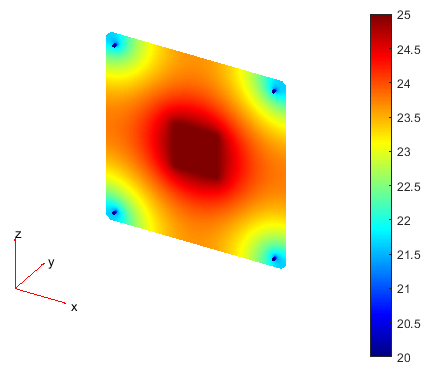
\includegraphics[scale=0.6]{base_temp_grad}
    \caption{A plot from an initial temperature test showing a 5 K temperature gradient over the receiver component baseplate when heated from below by a 40 W heat source placed at the plate's centre.}
    \label{fig:base_temp_grad}
\end{figure}
Following the results of this test, a secondary baseplate was installed below the initial baseplate with the two plates separated by a heatsink and an internal fan installed to promote air circulation throughout the front end. A follow-up test using this configuration returned a temperature gradient of 0.125 K across the component baseplate. A diagram of the completed setup is shown in \cref{fig:peltier_diag}
\begin{figure}
    \centering
    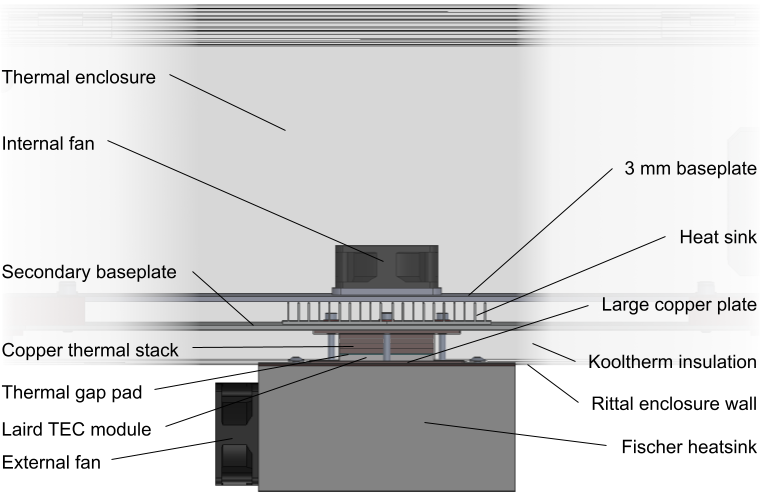
\includegraphics[width=\textwidth]{reach_peltier_diagram}
    \caption{A diagram representing the components for thermal conditioning of the receiver front-end. The vantage point shown is as if the front-end enclosure is laid on its back. It should be noted that the above figure is the MK II version which is slightly updated from the configuration currently deployed in the field.}
    \label{fig:peltier_diag}
\end{figure}

The TEC is controlled by an Electron Dynamics Southampton TC-M-U-10A module and powered by a separate custom-made 22 V power supply unit (PSU) designed to reduce RFI coupling from the very large switch currents produced. The PSU, shown in \cref{fig:psu}, is also configured to automatically power the external fan when the Electron Dynamics controller draws more than 6 W of power to prevent thermal overload.
\begin{figure}
    \centering
    \begin{subfigure}{.45\textwidth}
        \centering
        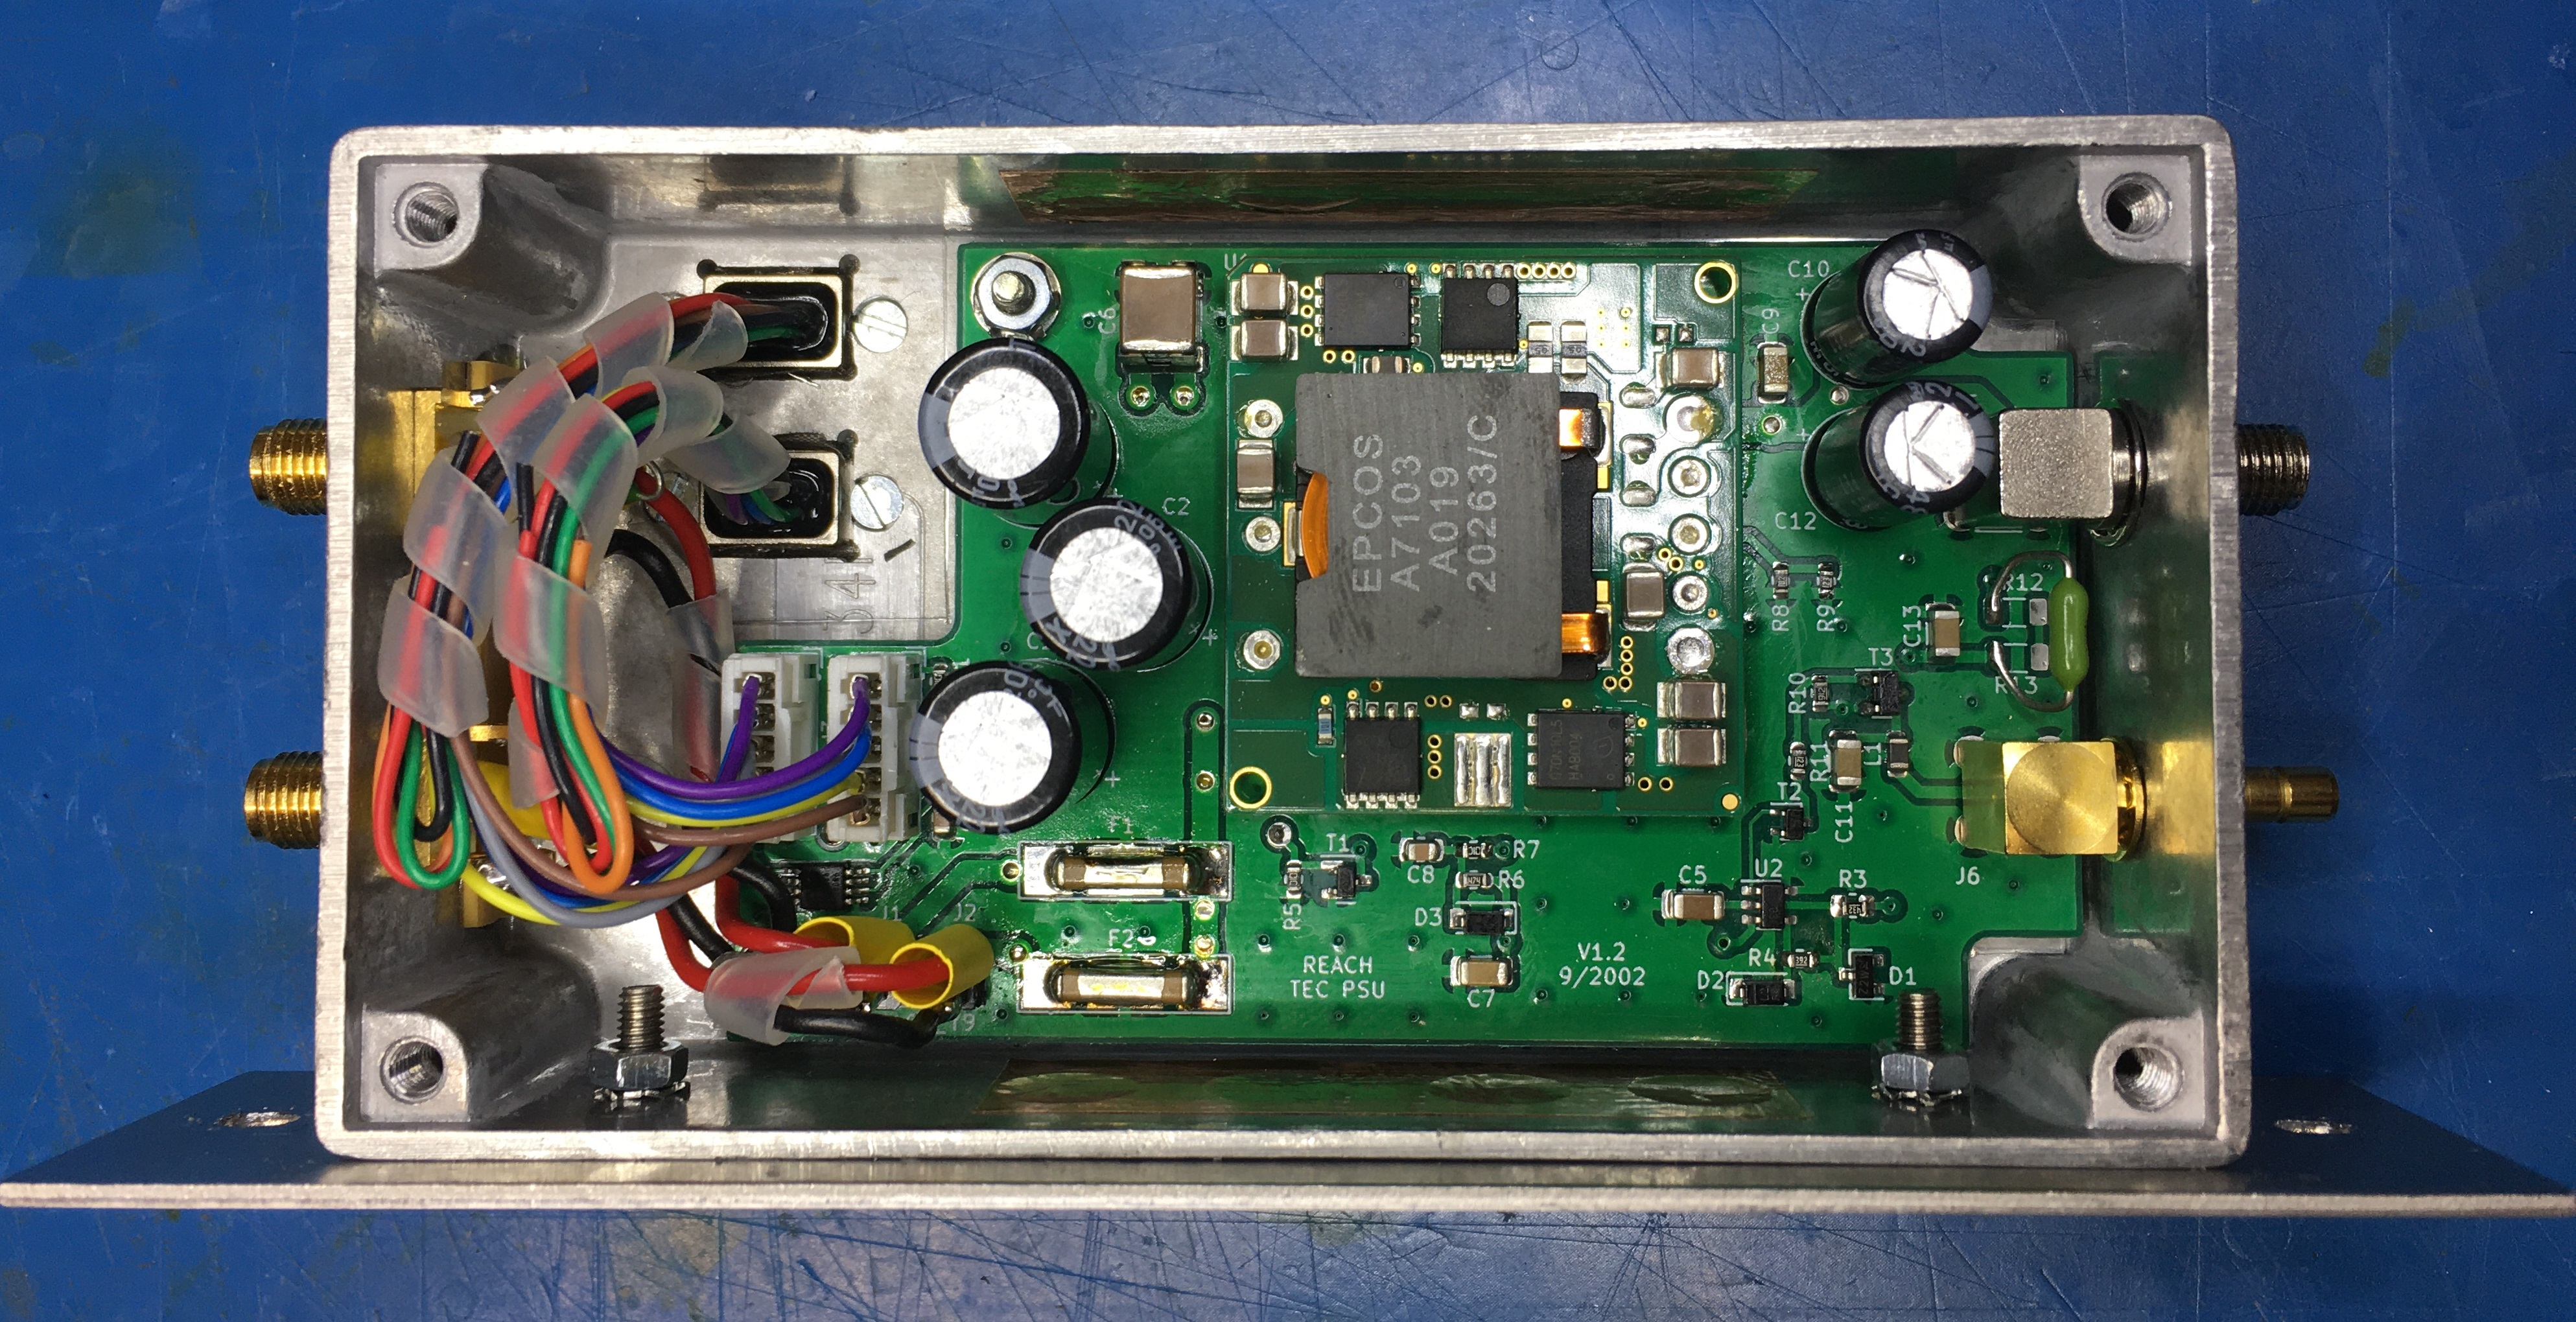
\includegraphics[width=\linewidth]{psu}
    \end{subfigure}
    \hfill
    \begin{subfigure}{.52\textwidth}
    \centering
        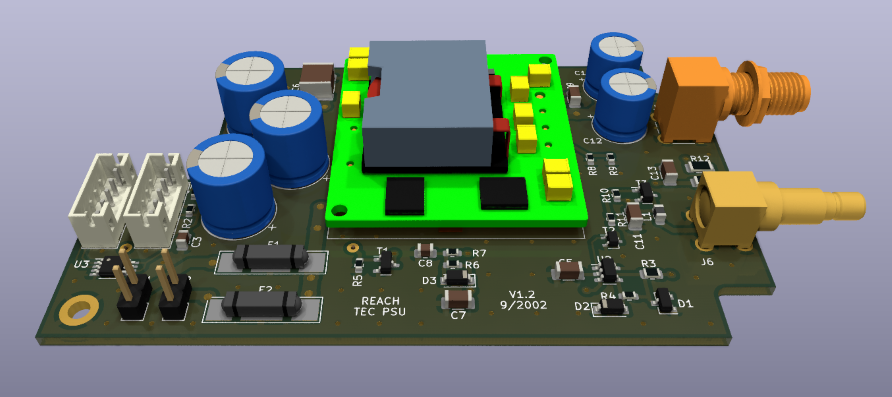
\includegraphics[width=\linewidth]{cad_psu}
    \end{subfigure}
    \caption{The constructed thermoelectric cooler power supply unit (left) along with its original CAD rendering (right) for perspective.}
    \label{fig:psu}
\end{figure}

The effectiveness of the front-end thermal management system was evaluated by testing the performance of the construction on 6 litres of bottled water placed in the empty front-end enclosure at room temperature with the TEC driven at its maximum 88 W and the Electron Dynamics controller instructed to maintain a $10^\circ$ C setpoint temperature as shown in \cref{fig:water_test} where the endpoint is achieved after about 8 hours of cooling with a steady-state temperature within 0.01 K of the target setpoint. These results suggest that a long, continuous amount of cooling is needed to stabilise the front-end temperature before calibration or observational measurements are made. This may be done in the afternoon or evenings preceding an observational run. OR FIND PLOT WITH TIME TAKES TO BRING FINALISED CONSTRUCTION TO SET POINT. An additional comparison of the completed thermal management system installed on the front-end enclosure with its 3D-rendered cross section is shown in \cref{fig:enclose_supp} for reference.
\begin{figure}
    \centering
    \centering
    \begin{subfigure}{.4\textwidth}
        \centering
        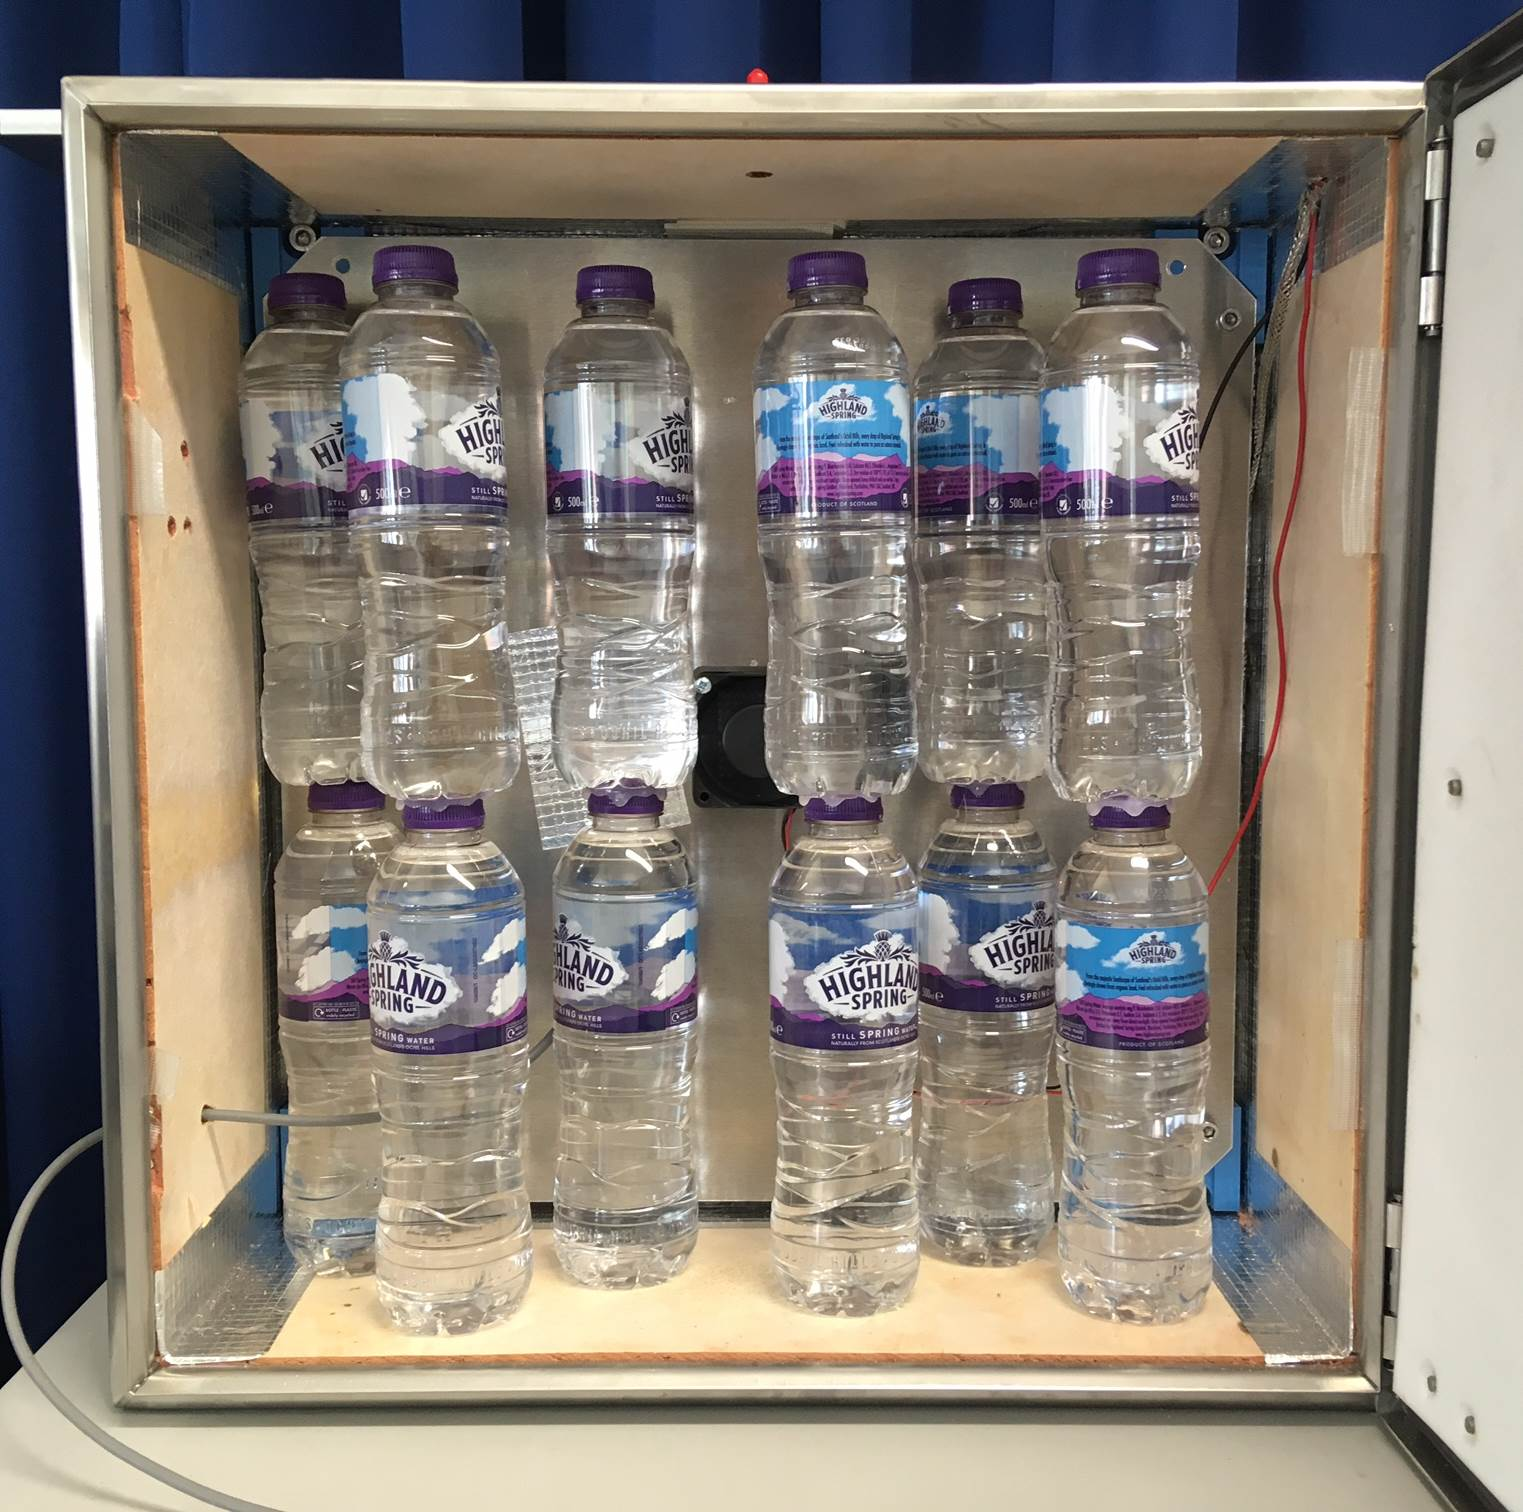
\includegraphics[width=\linewidth]{water}
    \end{subfigure}
    \hfill
    \begin{subfigure}{.55\textwidth}
    \centering
        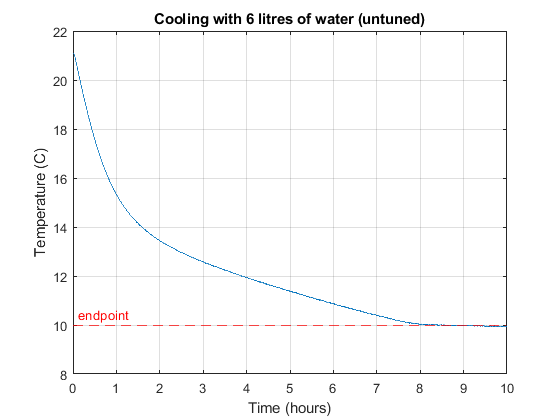
\includegraphics[width=\linewidth]{water_results}
    \end{subfigure}
    \caption{Six litres of water placed in the empty front-end enclosure with the thermal management system installed. The results of this test with the TEC driven at its maximum wattage and the controller setpoint of $10^\circ$ C is shown on the right. It should be noted that for this test, the proportional, integral and derivative controller values were not tuned beforehand, which reduces efficiency.}
    \label{fig:water_test}
\end{figure}


% =========================================
\subsubsection{Calibration sources}
One of the main obligations for thermal stability was to stabilise measurements of passive devices used to calibrate the instrument which we collectively refer to as ‘calibration sources’ or ‘calibrators’. Historically, absolute calibration is undertaken through measurement of each calibration source as part of a three-position Dicke cycle containing a single source, a reference $50 \Omega$ load and a reference noise source where comparison of power spectral measurements between the source and references serve to calibrate out time dependent system gain as detailed in REFERENCE Q-TERM EQUATION. Usually four sources were used; an ambient-temperature ‘\textit{cold}’ $50 \Omega$ load, a $50 \Omega$ load heated to high temperature, a cable shorted at one end and a cable left open at one end. The $50 \Omega$ loads give the absolute temperature scale in our calibration solution while the cables simulate antennas looking at an isotropic sky with temperatures equal to the cables’ physical temperature. A diagram of the Dicke switching procedure used in calibration is shown in \cref{fig:dicke}.
\begin{figure}
    \centering
    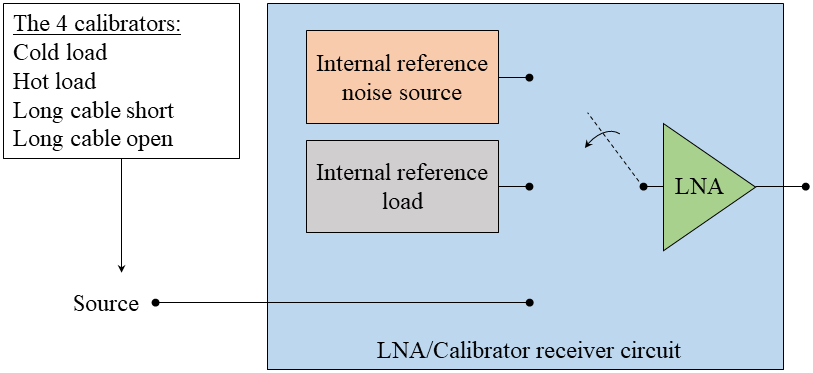
\includegraphics[scale=0.5]{dicke}
    \caption{A diagram of the Dicke switching procedure showing the calibrator position, $50 \Omega$ reference position and reference noise source position. Here, the four canonical calibration sources are used; the ambient and heated $50 \Omega$ loads along with the shorted and open cables. Power spectral measurements of these devices are conditioned by the Low Noise Amplifier (LNA) before being passed on to the spectrometer for initial removal of the time-dependant system gain.}
    \label{fig:dicke}
\end{figure}

The cold load used was taken from an 85033 $50 \Omega$ SMA calibration kit certified by Kirkby Microwave. Multiple heated loads were custom made for this experiment. A simple heated load was constructed from a 4-inch RG-405 coaxial cable terminated with a $50 \Omega$ load attached to a proportional heater connected to DC power with the temperature directly monitored through contact with a thermocouple. As the heated calibration source is typically heated to $\sim 370$ K, which could affect the temperatures of nearby ambient components, an improved calibrator was constructed with the $50 \Omega$ resistor and thermistor attached to a 4-inch semi rigid cable surrounded with thermal insulation and encased in an acrylic cubic shell. A temperature gradient across the 4-inch cable within the construction is produced by the temperature difference between the heated load and the coaxial end connected to the receiver input. As this changes the temperature ‘seen’ by the instrument, a corrective factor is introduced in our calibration calculations and detailed in REFERENCE TEMPERATURE CORRECTION SECTION. While this advanced heated load was used for some of the results presented in this work such as in FORWARD REFERENCE SECTIONS, the simple heated load was the device deployed to the field due to time constraints impacting critical adjustments to reinforce the advanced heated load. A diagram of the advanced heated load is included in \cref{fig:hot_load}.
\begin{figure}
    \centering
    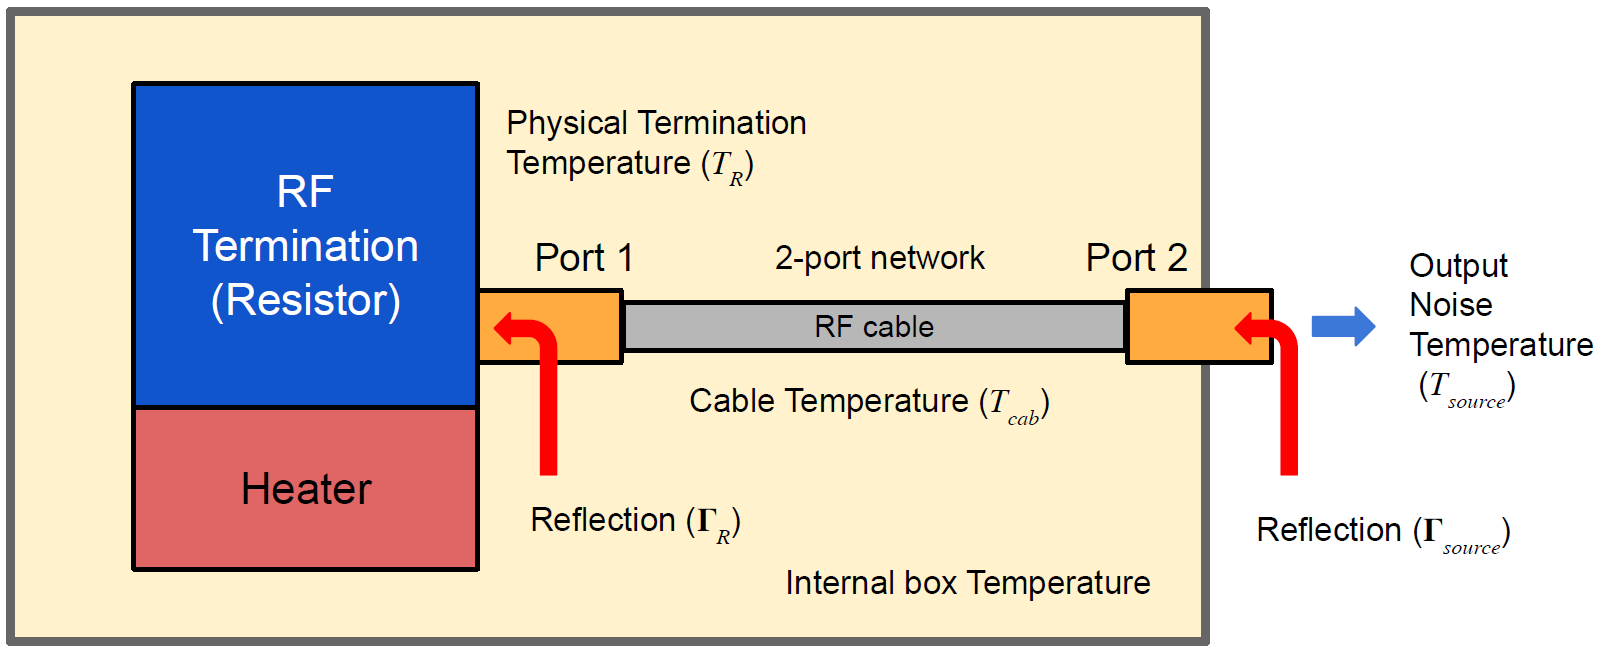
\includegraphics[width=0.65\textwidth]{hot_load}
    \caption{Illustration of the heated load construction for use as a calibration source. The thermally enclosed resistor and powered heater are connected to the input switch via a 4-inch cable as shown in the diagram. These components effectively form a temperature gradient across the calibration device which must be corrected for via the procedure discussed in REFERENCE TEMPERATURE CORRECTION SECTION as $\T{R}$, $\T{cab}$ and $\T{source}$ are not necessarily equal.}
    \label{fig:hot_load}
\end{figure}

Open and shorted coaxial terminations were taken from the same Kirkby 85033 kit and connected to the end of coaxial cables. Over the course of receiver development, many different models and lengths of cables with varied specifications were tried with the final deployed system having the open and shorted ends connected to 10 metre LMC195 coaxial cabling partially built in-house at Cambridge. With the need for more accurate characterisation of the instrument, we have expanded our selection of calibration sources to twelve, maximising the information detailing the instrument response. Additional ambient-temperature $25 \Omega$ and $100 \Omega$ resistors were included for increased data on non-complex impedance response. The same 10 metre LMC195 cable was also terminated with $10 \Omega$ and $250 \Omega$ resistors. An additional 2 metres of LMC195 terminated with $27 \Omega$, $36 \Omega$, $69 \Omega$ and $91 \Omega$ resistors was also included. These additional terminations were all custom made in Cambridge.

The calibration sources and resistances were carefully chosen to permit strategic sampling of the noise waves as a function of impedance. \Cref{fig:smith} demonstrates the extensive scope of frequency-dependent impedances for our calibration sources as well as a simulated impedance of the REACH dipole antenna covering 50--150 MHz.
\begin{figure}
    \centering
    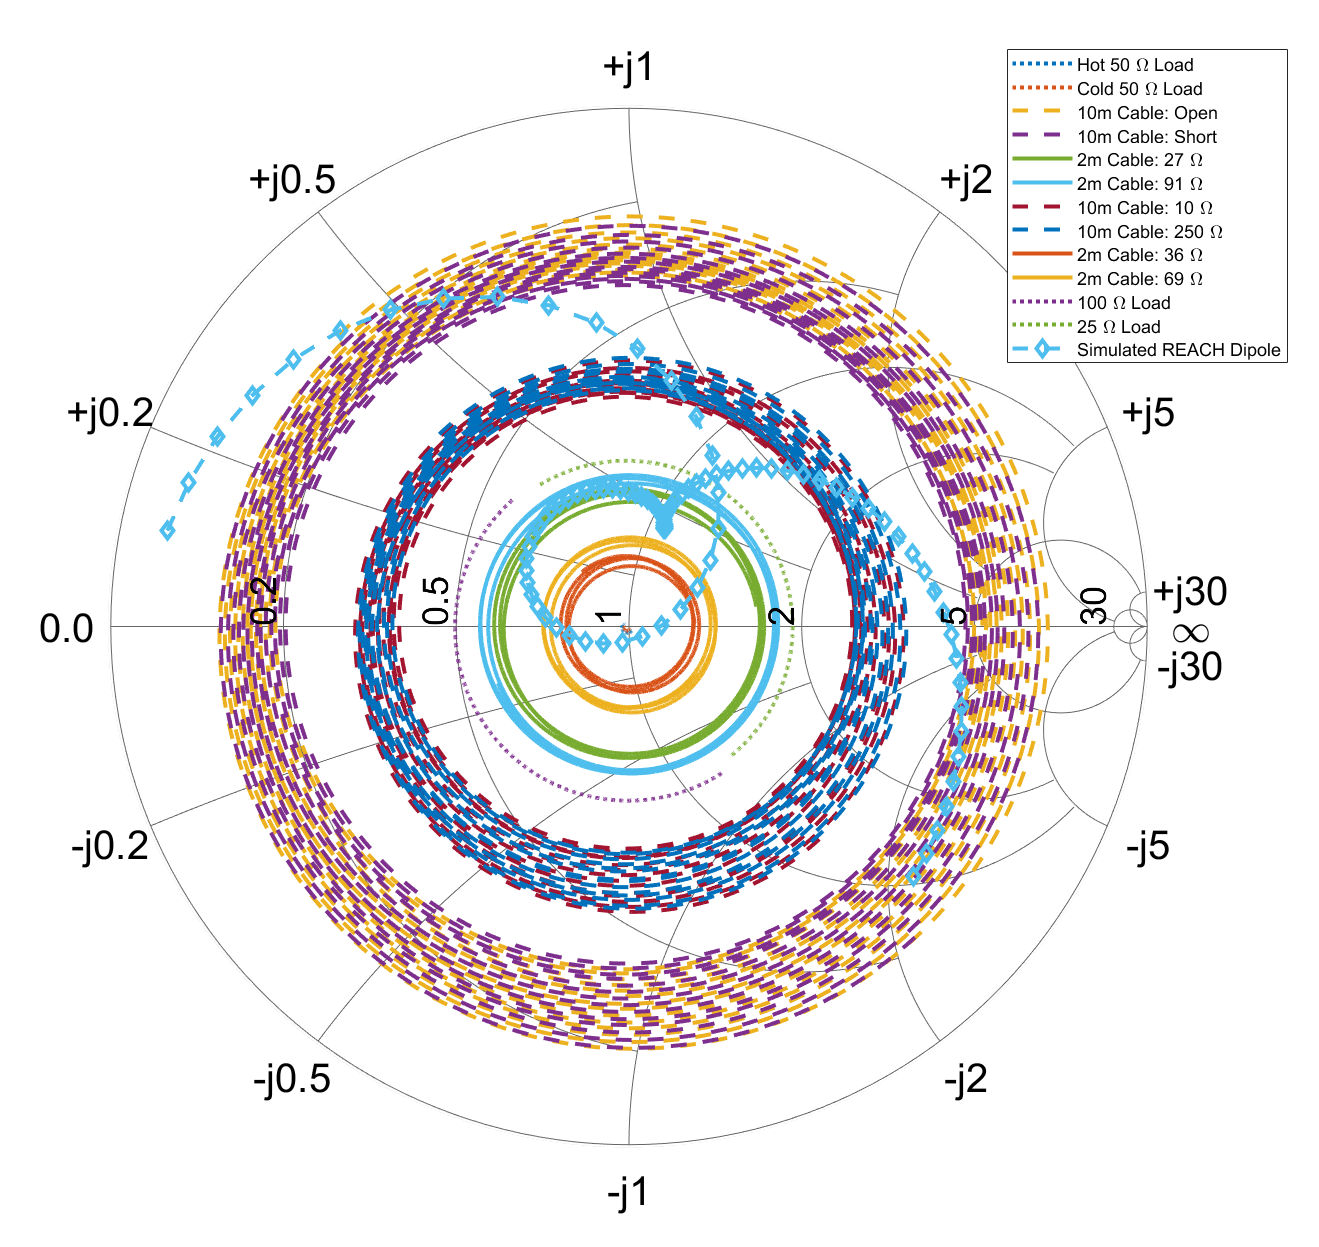
\includegraphics[scale=0.3]{smith}
    \caption{Smith Chart showing the impedance of twelve calibration sources and the simulated REACH antenna (internal variant \#0744) with the centre of the plot indicating an impedance of 50 $\Omega$. The plot ranges from 50--150 MHz with the antenna curve starting at 50 MHz on the left-hand side. The extensive coverage in impedance space by our calibration standards can be interpreted as a substantial amount of information regarding the characteristic response of the instrument. Note that the impedances of the ambient and heated 50 $\Omega$ loads lie directly in the middle of the chart and are partially obscured by the antenna plot. Updated from figure included in REFERENCE REACH NATURE PAPER}
    \label{fig:smith}
\end{figure}
\Cref{fig:smith} also demonstrates measurements of the $25 \Omega$ and $100 \Omega$ loads as half circles on the Smith chart, which differs from the theoretical points at $25 \Omega$ and $100 \Omega$ due to the practical limitations of real-world impedance measurement and exacerbated by the additional RF path in our receiver between the sources and the measurement reference plane for the reflection coefficients. These effects were the motivation for the corrections detailed in REFERENCE S11 CORRECTION MATHS SECTION.

Power spectral measurements are taken of two reference sources for every measurement of a calibration source to divide out the short-time variability in receiver gain as previously stated. Ideally, the reference load would be a separate $50 \Omega$ load of high quality such as from an additional certified calibration kit, but due to time constraints in the deployment, a repeated measurement of the ambient load used as a calibration source was taken. As these Dicke switch measurements detail the changing gain of the system and not the absolute differences between the devices used as calibration sources and reference sources, we believe that this degeneracy would not severely impact the quality of the results presented in this work.

The reference noise source used is a Noisecom NC346A. An important distinction must be made here between the heated $50 \Omega$ load as a calibration noise source and the Noisecom noise diode used as a reference noise source. While the constant noise power provided by the noise diode is necessary for maximal radiometer measurement accuracy through removal of the time-dependent gain fluctuations via the Dicke switching procedure, the direct and accurate measurement of the heated $50 \Omega$ load via thermocouple is beneficial for the removal of systematic noise via accurate noise wave parameter derivation. 

Noise output data of the reference noise diode as provided in decibel excess noise ratio by Noisecom in shown in \cref{tab:ns_noise}.
\begin{table}
    \begin{center}
    \begin{tabular}{ |c|c| }
        \hline
        {Frequency} & {Excess noise ratio} \\
        \hline
        30 MHz & 6.05 dB \\
        40 MHz & 6.03 dB \\
        50 MHz & 6.00 dB \\
        60 MHz & 5.94 dB \\
        70 MHz & 5.91 dB \\
        80 MHz & 5.87 dB \\
        90 MHz & 5.84 dB \\
        100 MHz & 5.79 dB \\
        110 MHz & 5.80 dB \\
        \hline
    \end{tabular}
    \quad
    \begin{tabular}{ |c|c| }
        \hline
        {Frequency (contd.)} & {Excess noise ratio (contd.)} \\
        \hline
        110 MHz & 5.80 dB \\
        120 MHz & 5.77 dB \\
        130 MHz & 5.80 dB \\
        140 MHz & 5.81 dB \\
        150 MHz & 5.83 dB \\
        200 MHz & 5.88 dB \\
        250 MHz & 5.87 dB \\
        350 MHz & 5.87 dB \\
        500 MHz & 5.89 dB \\
        \hline
    \end{tabular}
    \end{center}
    \caption{Manufacturer quoted noise output for the Noisecom NC346A noise diode used as the reference noise source within the Dicke switching procedure as an excess noise ratio. The stability of the noise output within the REACH observational band (50 -- 130 MHz) at these scales should be noted, which is beneficial for the removal of time-dependent system gain.}
    \label{tab:ns_noise}
\end{table}
We can convert the noise output values from \cref{tab:ns_noise} to linear scale using the equation
\begin{equation}
    \mathrm{ENR_{dB}} = 10 \cdot \log_{10} \left( \frac{\mathrm{T} - 290}{290}\right)
\end{equation}
with 290 being the standard reference temperature for noise and $\mathrm{T}$ as a linear-scale excess noise above ambient temperature (assumed to be 298 K). A plot of the linear noise output of the reference noise diode with ambient temperature subtracted is provided in \cref{fig:ns_diode} which may serve as a potential sanity check for our calibration algorithm as these values inform us of the approximate values of the $\T{NS}$ noise wave parameter as detailed in REFERENCE RECEIVER MATHS SECTION and verified in REFERENCE NIMA MATLAB RESULTS SECTION. This value may not be exactly replicated however, due to the additional RF path introduced earlier and again detailed in REFERENCE S11 CORRECTION MATHS SECTION. It should also be noted that these values are exclusive to this particular noise source and the use of different noise diodes in future builds, including identical model numbers, would necessarily be different and require recalculation following the above prescription.
\begin{figure}
    \centering
    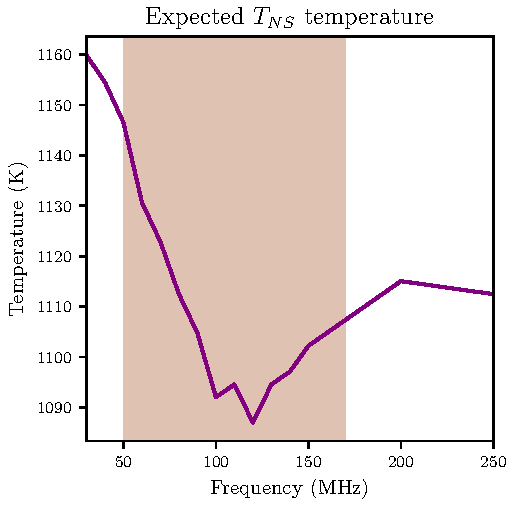
\includegraphics[width=0.5\textwidth]{ns_diode}
    \caption{A plot of the reference noise diode output from the datasheet provided by Noisecom. The scale of the plot gives us a value expected of the $\T{NS}$ noise wave parameter from our calibration algorithm. As shown, the output of the diode is essentially stable at these high temperature scales but cannot be measured accurately in the field due to the output being an effective noise temperature from a diode imitating the noise of a black body at such a temperature. The shaded region is the REACH observational band 50--130 MHz.}
    \label{fig:ns_diode}
\end{figure}


% =========================================
\subsubsection{Switches}
The sizeable battery of calibration and reference sources may seem at first glance to run against the primary goal of having a small-volume receiver. To meet this challenge, a complicated network of mechanical switches was conceived to allow for the myriad components and various signal paths through the instrument. The essential calibration sources mentioned in the previous subsection were gathered on an 8-way switch (referred to as MS1) with switch positions one through six taken up by the antenna, cold load, reference noise source, heated load, $25 \Omega$ load and $100 \Omega$ load respectively. To avoid the size requirements of having multiple calibration cables with various terminations, a single 2 metre LMC195 cable and 10 metre LMC195 cable were connected to MS1 positions seven and eight with the opposing ends of the cables connected to their own 4-way switch referred to as MS3 and MS4 respectively. These cable switches were connected to the appropriate terminations according to the previous subsection; $36 \Omega$, $27 \Omega$, $69 \Omega$ and $91 \Omega$ for MS3 positions one through four as well as open termination, shorted termination, $10 \Omega$ and $250 \Omega$ for MS4 positions one through four for the 2 metre and 10 metre cables. A custom 3D-printed structure was designed to house the two calibration cables within the receiver front-end which is highlighted in \cref{fig:stadium}
\begin{figure}
    \centering
    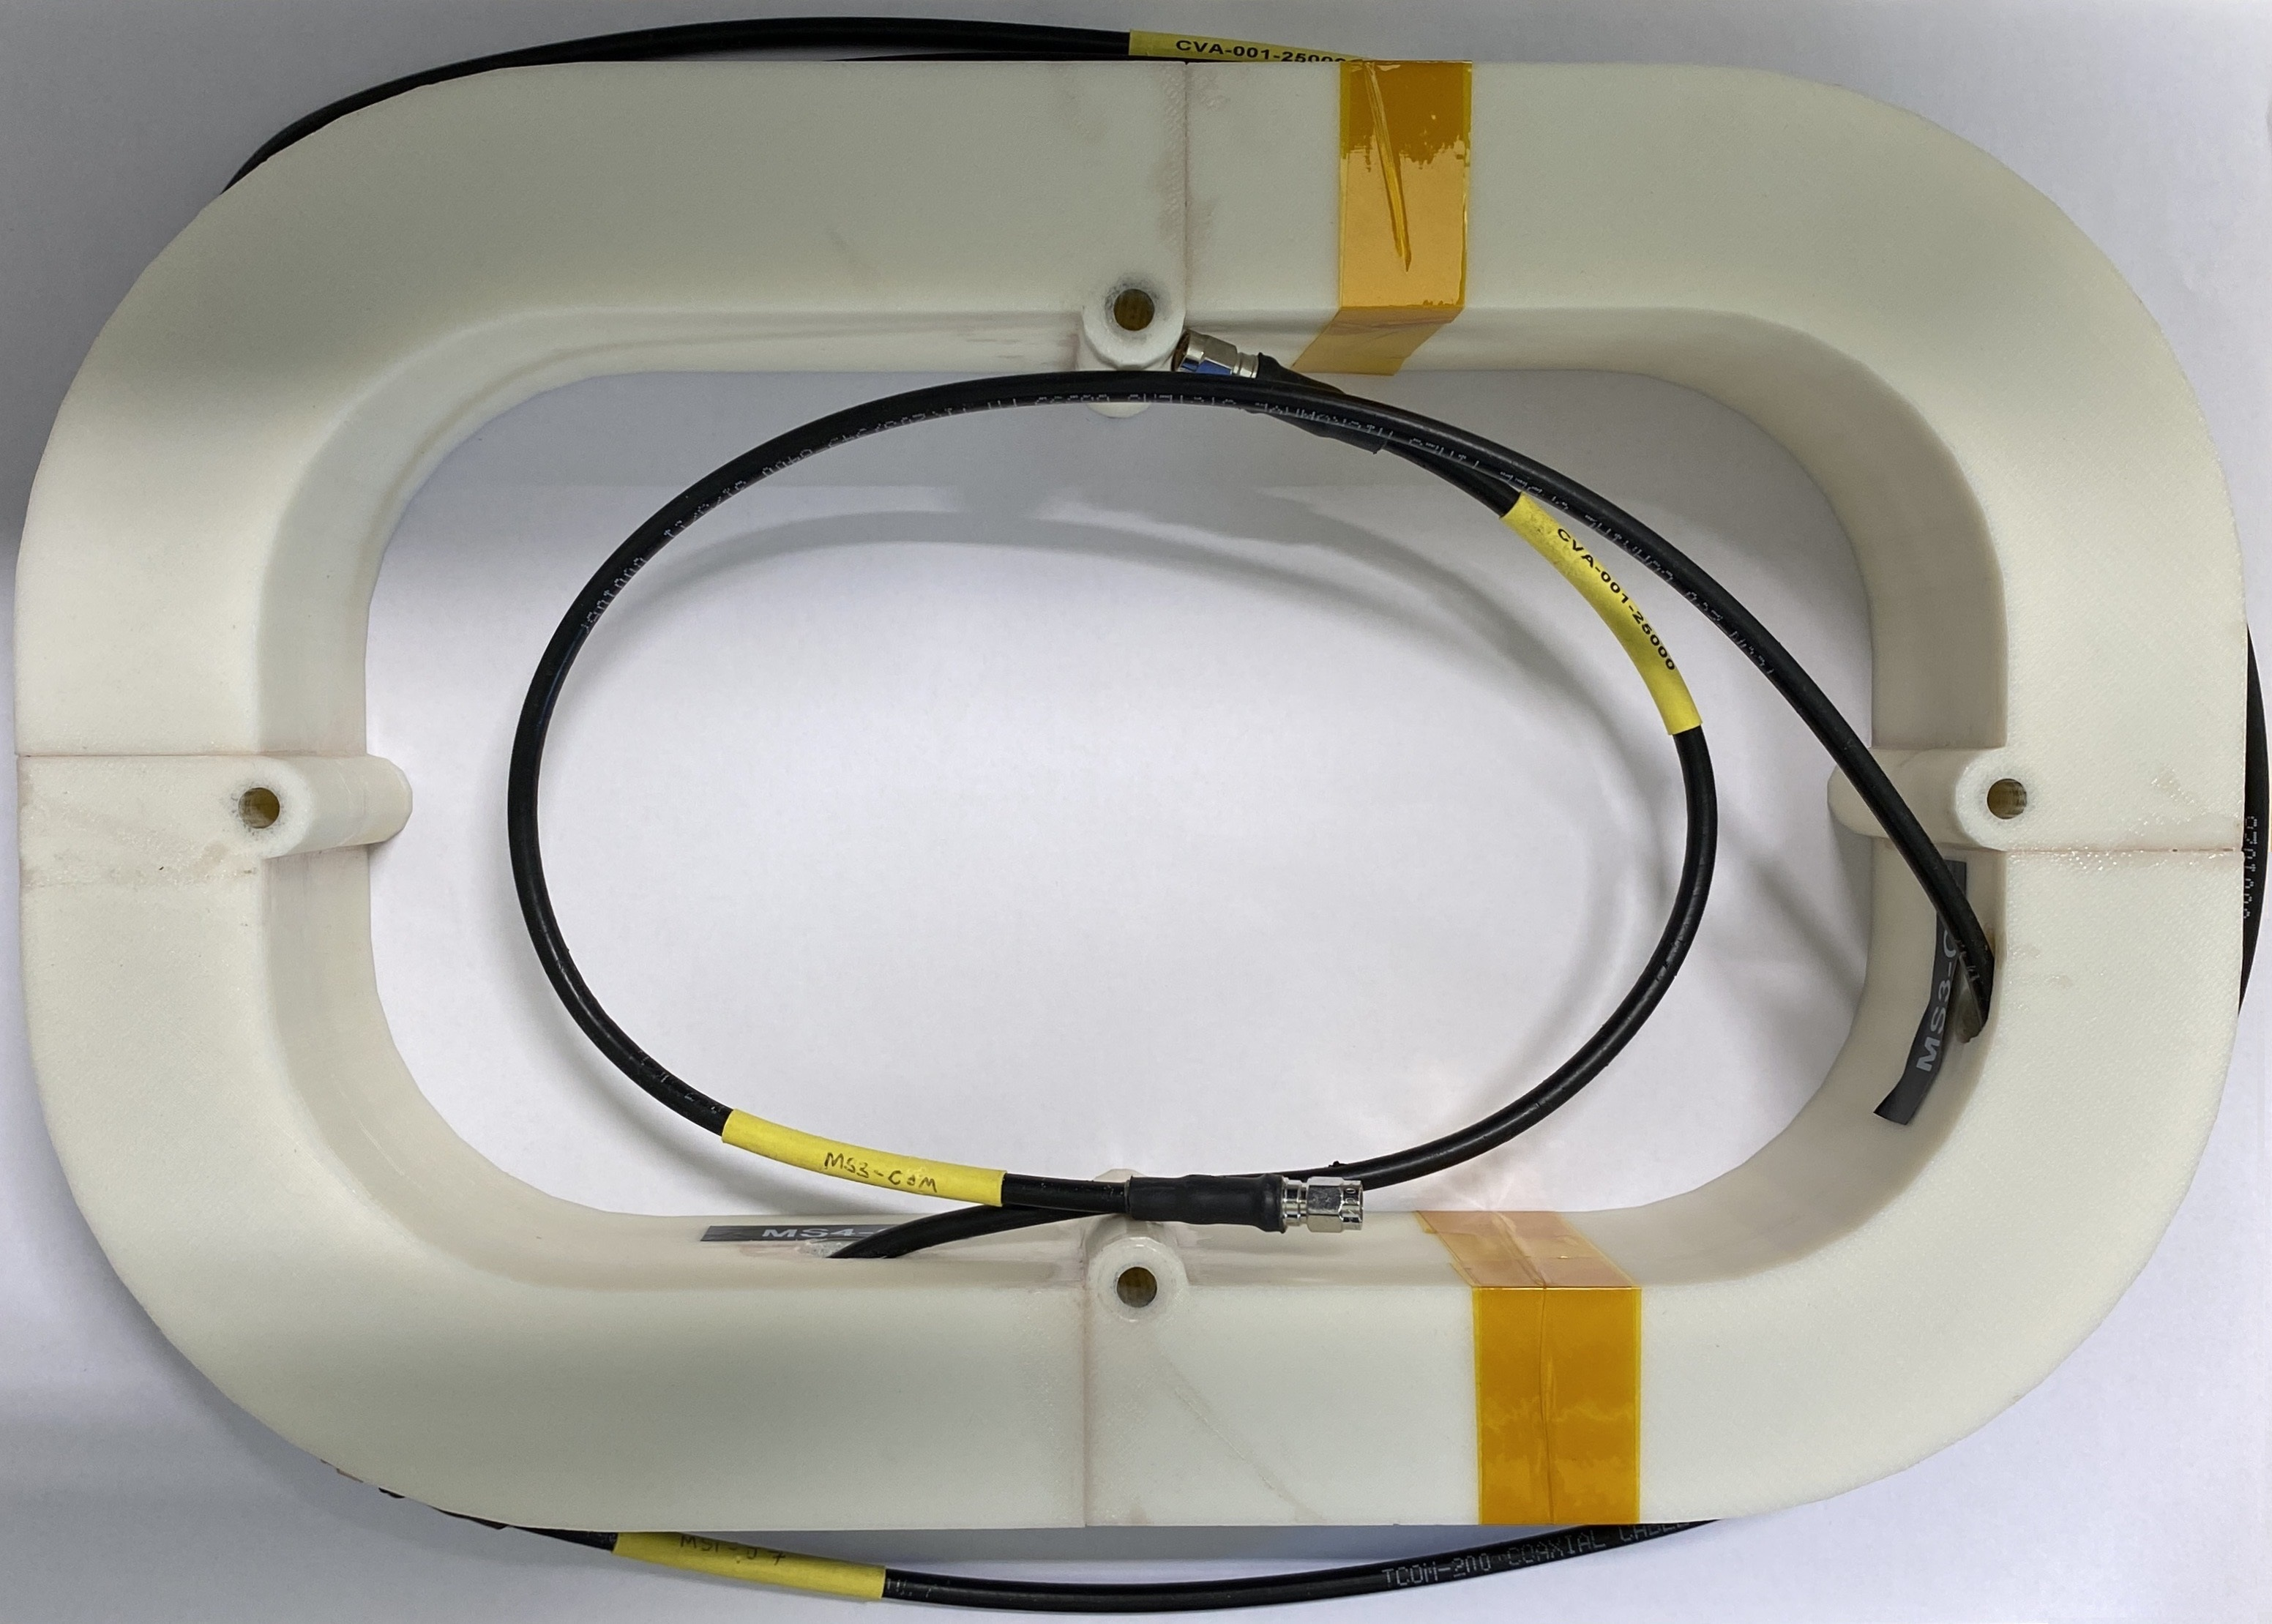
\includegraphics[width=0.65\textwidth]{stadium}
    \caption{3D printed housing for the 2 metre and 10 metre calibration cables. This unit is affectionately referred to as ‘the stadium’.}
    \label{fig:stadium}
\end{figure}

A schematic block diagram of the switching configuration is shown in \cref{fig:overview}.
\begin{figure}
    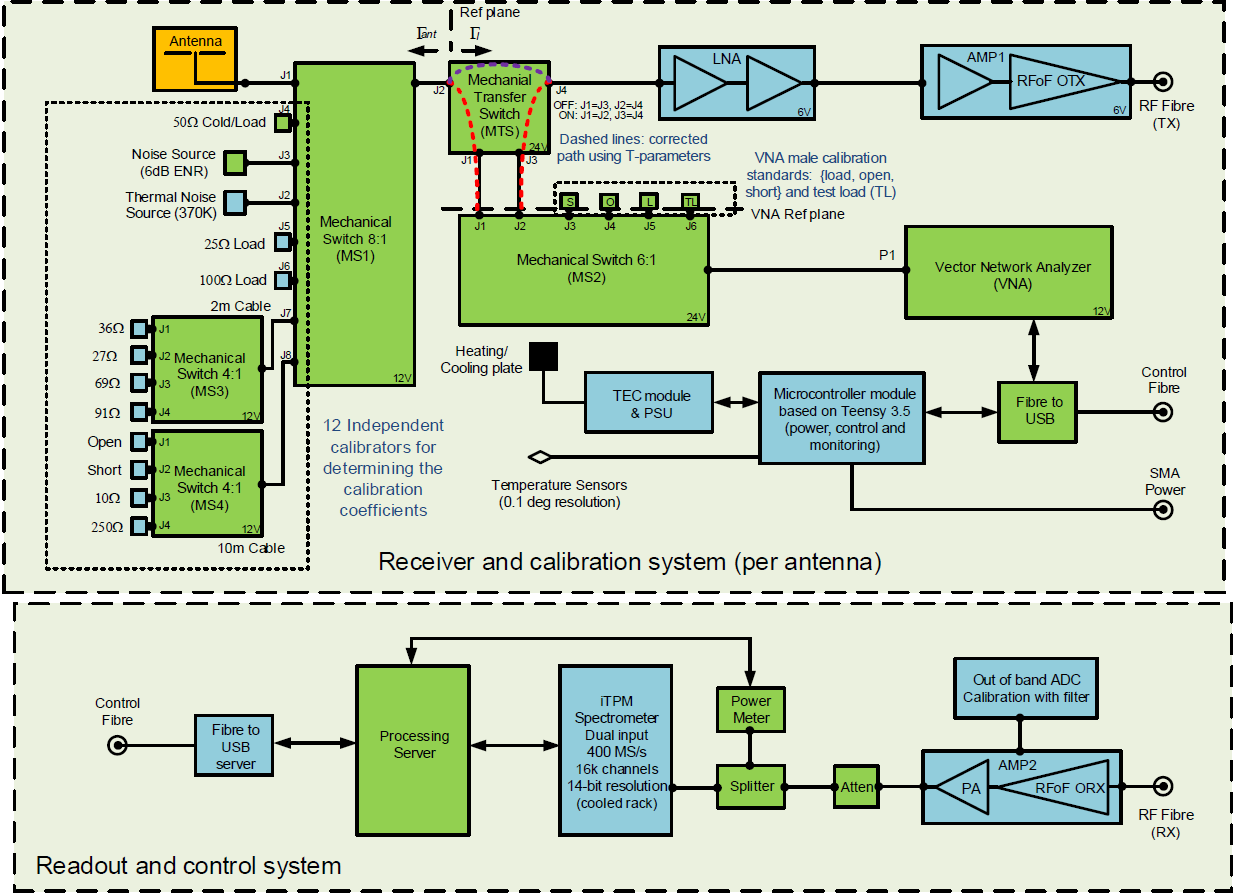
\includegraphics[width=\columnwidth]{radiometer_v8a}
    \caption{An overview of the REACH radiometer showing calibration sources and the antenna connected to an 8-way mechanical input switch at the receiver input. The green sub-blocks represent off-the-shelf components, whilst blue represent custom designs. $\Gamma_{ant}$ represents the reflection coefficient of the antenna or calibrator, $\Gamma_{l}$ is the reflection coefficient of the low noise amplifier (LNA). The red dashed line represents the extra path measured by the VNA that is not present during spectral measurements while the purple dashed line is the path present exclusively during spectral measurements. Corrections for these additional paths are detailed in REFERENCE SPARAMETER CORRECTION SECTION. ‘ENR’ is the Excess Noise Ratio of a Noisecom NC346A noise source; ‘OTX’ indicates an optical transmitter; ‘TX’ indicates transmission mode; ‘TEC’ stands for Thermoelectric Cooling; ‘SMA’ is a SubMiniature version-A connector; ‘PA’ is Power Amplifier; ‘RX’ indicates reception mode and ‘Atten.’ represents a signal attenuator. Updated from figure included in REFERENCE REACH NATURE PAPER OR NIMA PAPER.}
    \label{fig:overview}
\end{figure}
As shown, a Mechanical Transfer Switch (MTS) facilitates pathways to the Low Noise Amplifier (LNA) and Vector Network Analyser (VNA) for spectral and reflection measurements respectively. MTS position two connects directly to the 8-way switch housing the calibration sources and MTS position four leads to the LNA/spectrometer pathway. The first and third MTS switch positions connect to the first two positions of a 6-way switch (MS2) that direct to the VNA. MS2 positions three through six connect to additional calibration standards used to separately calibrate the VNA before measurement as detailed in a following VNA subsection. For all of the connections detailed here, male sources and terminations were connected to female switch connections to avoid reflections that would spawn from the inclusion of male-female adaptors\footnote{or ‘worms’ as they are colloquially referred to.}

An effort was made to reduce any negative effects presented to the instrument by this network of switches. Mechanical switches were implemented over the alternative electronic switches due to the lower signal loss of the former. The Mini-Circuits absorptive switches chosen exhibit 0.01 dB loss within the REACH observational band with better than 100 dB isolation to reduce the radio-frequency leakage into the rest of the signal chain. Extra shielding was added to the switch drivers to further reduce self-induced RFI as shown in \cref{fig:switches}. The 20 mm trace length of the mechanical switch drivers was mitigated by placing the drivers as close to the switch as possible followed with the inclusion of custom 3D-printed connection covers coated with conductive paint.
\begin{figure}
    \centering
    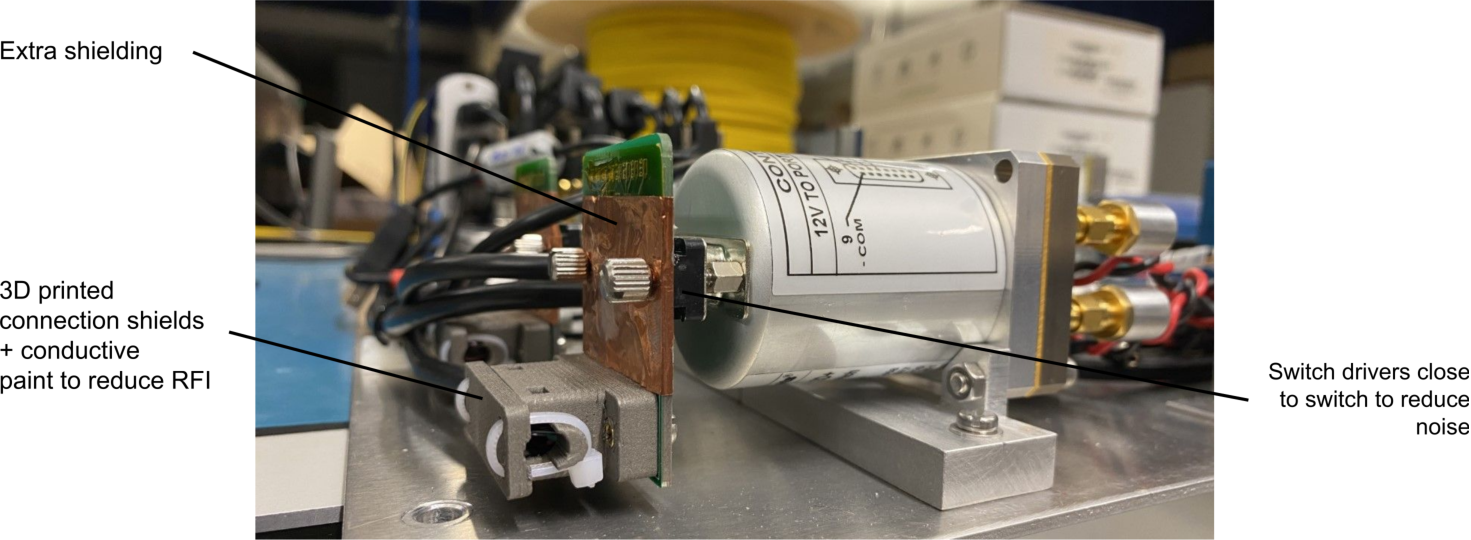
\includegraphics[width=\textwidth]{switches}
    \caption{A mechanical switch installed on the front-end component plate showing the extra shielding, 3D-printed housing and close placement of switch drivers.}
    \label{fig:switches}
\end{figure}
A table of the mechanical switches used is presented in \cref{tab:switches} for reference and a table with the contents of each switch connection detailed in \cref{tab:switch_content}. An mock-up of the switch configuration for a reflection coefficient measurement of the open-ended 10 metre cable is provided in \cref{fig:switch_mock} for illustrative purposes as well.
\begin{figure}
    \centering
    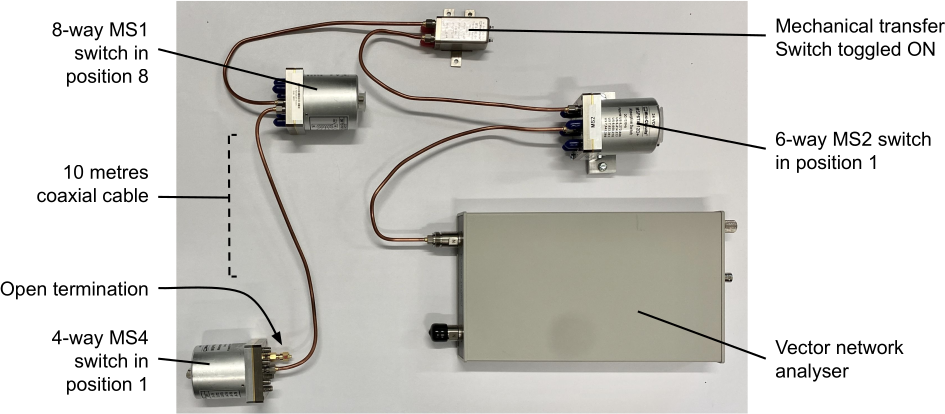
\includegraphics[width=\textwidth]{switch_example}
    \caption{A mock-up of the components and configuration needed for a reflection coefficient measurement of the open-ended 10 metre cable using parts from the receiver (except for the 10 metre cabling which was too long.). For this measurement, the open termination connected to the MS4 switch input port 1 with the MS4 switch toggled to position 1 via command line interface. The MS4 switch output is connected to the 10 metres of LMC195 cabling with the other end of the LMC195 cable connected to the port 8 input of the MS1 switch. The MS1 switch is toggled to position 8 via CLI. The MS1 output connects to the port 2 input of the MTS switch followed by a connection to the port 1 input of the MS2 switch. With the MS2 switch toggled to port 1, the MS2 output should connect to the VNA input allowing for a connection to the opened termination though the MS2, MTS, MS1 and MS4 switches. This configuration allows for a reflection coefficient measurement of the opened termination by the VNA.}
    \label{fig:switch_mock}
\end{figure}


% =========================================
\subsubsection{The microcontroller unit}
As with most modern instruments, control an monitoring of the receiver front-end and its individual components is overseen by a central device. This control unit is required to initialise the specific switch positions needed for measurements as seen in \cref{fig:overview}. As an unmanned experiment in the South African Karoo, the capability for resetting components, especially during remote triage, is another critical function of the controller unit. With 88 necessary connections to oversee within the receiver front-end, construction of an adequate controller using off-the-shelf components would ordinarily take the space of a standardised 19-inch rack ($\sim 48$ cm\textsuperscript{2}). This along with the low noise requirements and restricted power budget of the REACH experiment prompted the development of a novel control unit design; a miniaturised management device or, ‘microcontroller unit’\footnote{Also abbreviated as ‘$\mu$con’ for short.}. Much of the compactness of our miniaturised control unit can be attributed to a careful consideration in constituent components however, an innovative stacked dual-board design allowed us to reduce the size by an order of magnitude condensing the microcontoller unit into a $13 \times 12 \times 10$ cm volume.

The first of the two boards in our microcontroller unit is the control board mounted by a PJRC Teensy 3.5 development board\footnote{Teensy 4.X is suggested for any future receiver designs due to the anticipated permanent reduction in supply of the 90 nm silicon MK64FX512VMD12 chips constituent to the Teensy 3.5. Newer Teensy boards boasting 45 nm chips may also provide increased efficiency and capability in subsequent builds.} based on the Arduino infrastructure. The Teensy board, as shown in \cref{fig:teensy} contains 64 digital input/output ports assigned to individual switch configurations facilitating component control through a USB serial interface.
\begin{figure}
    \centering
    \begin{subfigure}{0.5\textwidth}
        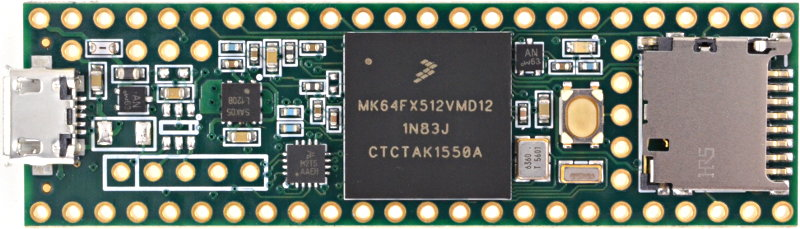
\includegraphics[width=\textwidth]{teensy_top}
    \end{subfigure}
    \begin{subfigure}{0.5\textwidth}
        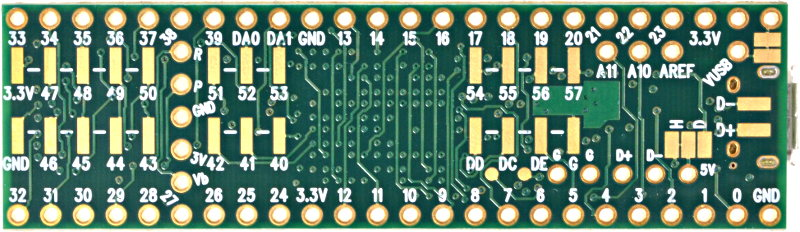
\includegraphics[width=\textwidth]{teensy_bottom}
    \end{subfigure}
    \caption{The front and back of the Teensy board is shown in the top and bottom respectively. Along the edges of the board are the input/output connectors (yellow-outlined white circles) which are paired to specific mechanical switch configurations throughout the front-end.}
    \label{fig:teensy}
\end{figure}
The $110 \times 90$ mm control board upon which the Teensy board is mounted to also contains the 48 V power input from the solar panels as well as 12 V and 5 V outputs for front-end components and can be seen in \cref{fig:control_board}.
\begin{figure}
    \centering
    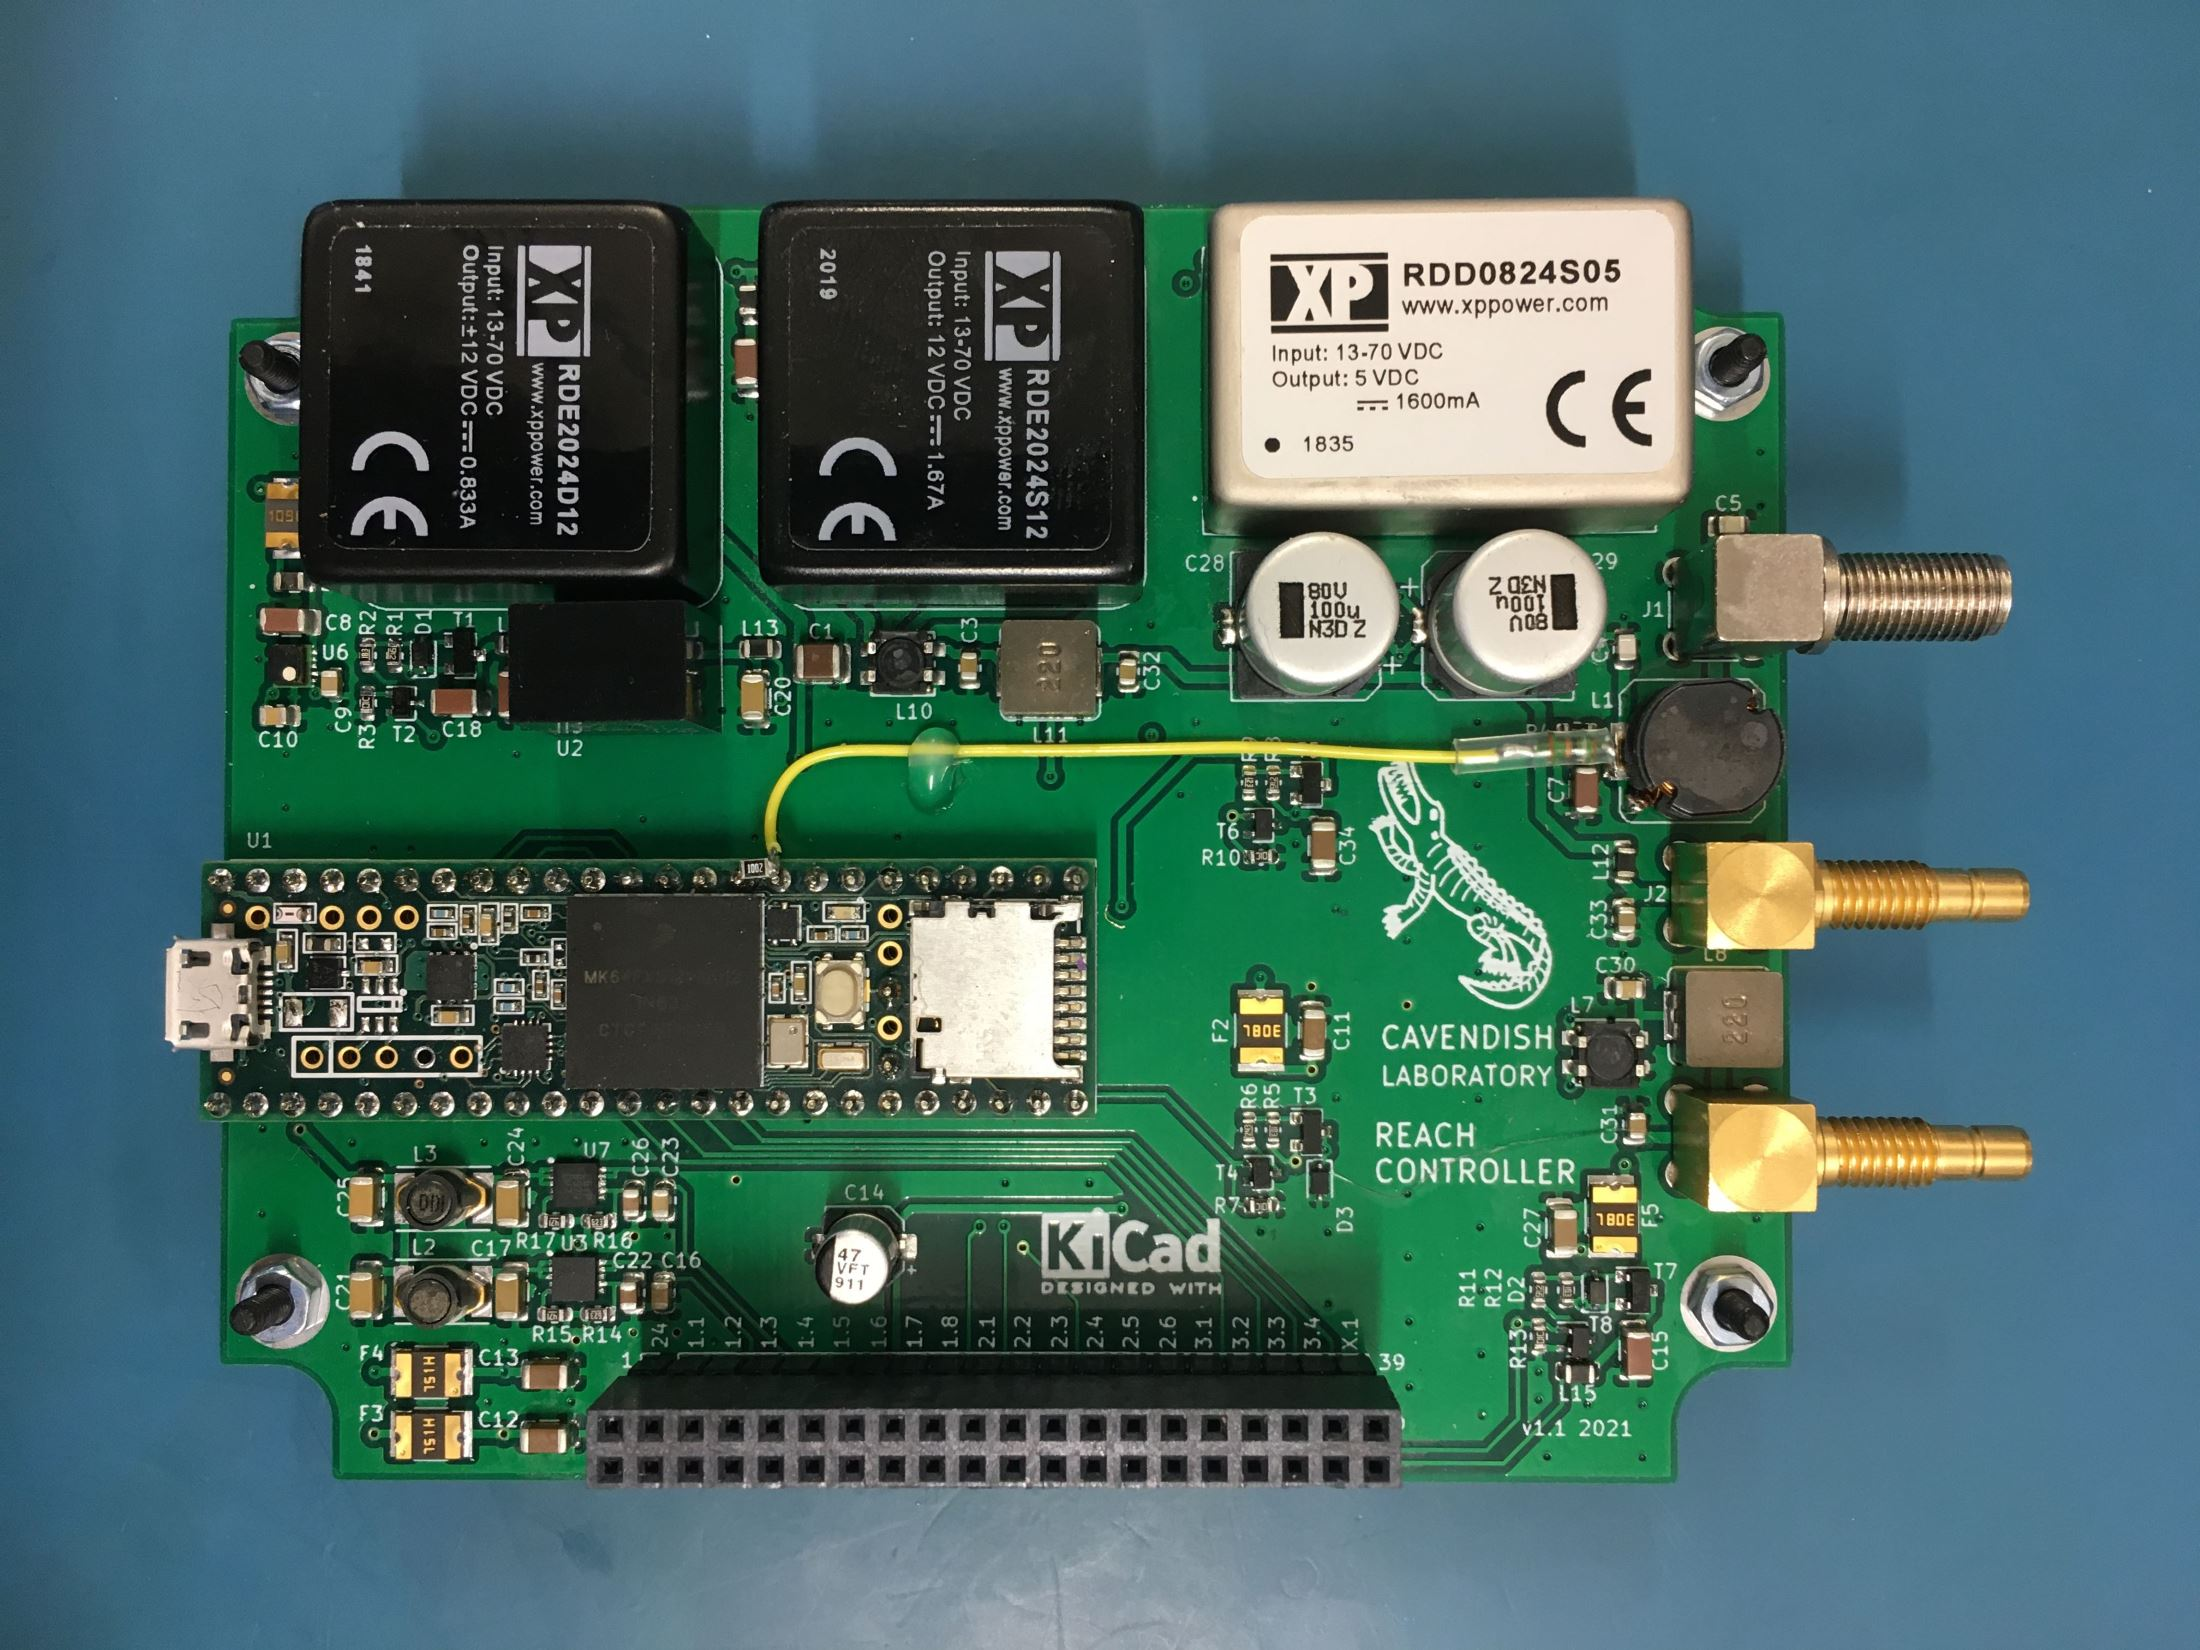
\includegraphics[width=0.5\textwidth]{control_board}
    \caption{The microcontroller unit control board with the Teensy board mounted at the left centre. The 48 V in, 12 V and 5 V out can be seen on the right of the board serving a portion of the overall microcontroller unit's power distribution functionality.}
    \label{fig:control_board}
\end{figure}
The controller board also incorporates RFI filtering and I\textsuperscript{2}C bus subsystems for ancillary device control such as the external fan.

Stacked above the controller board is the breakout board as shown in \cref{fig:break_board} which is primarily responsible for the remaining front-end connections but also a 28 V noise source regulator, 6 V power supply and additional EMI filtering.
\begin{figure}
\centering
    \centering
    \begin{subfigure}{.5\textwidth}
        \centering
        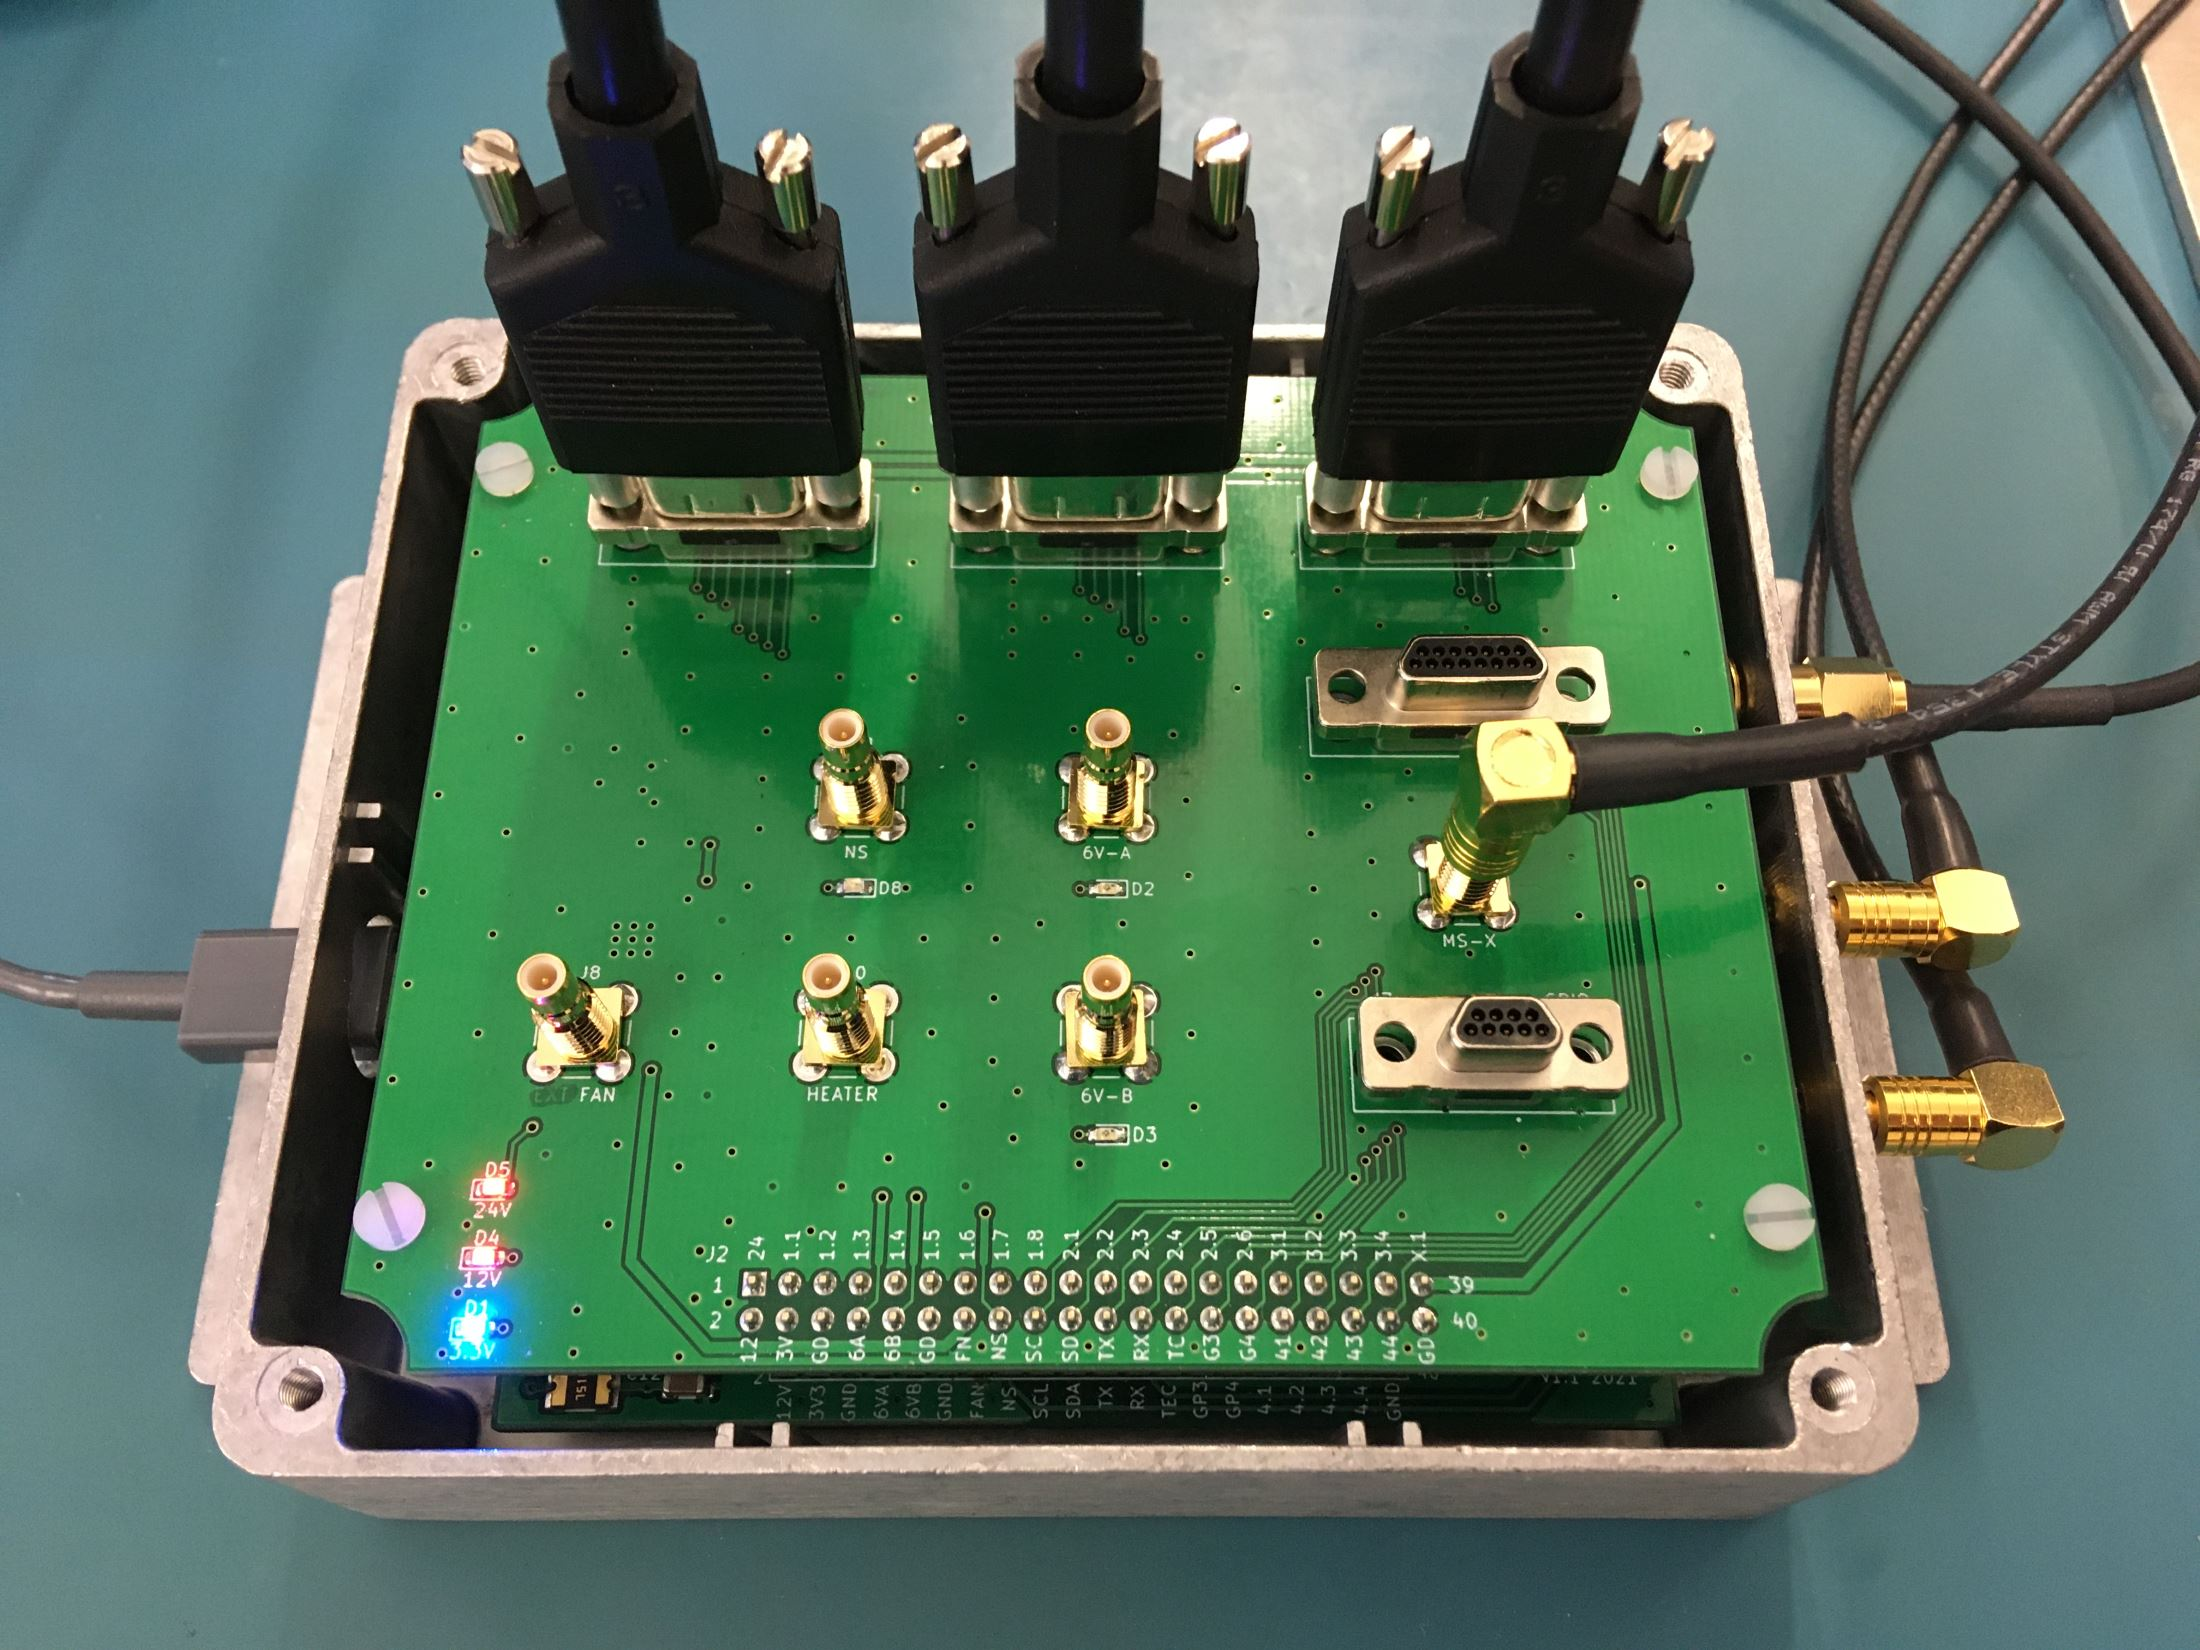
\includegraphics[width=\linewidth]{ucon}
    \end{subfigure}
    \hfill
    \begin{subfigure}{.45\textwidth}
    \centering
        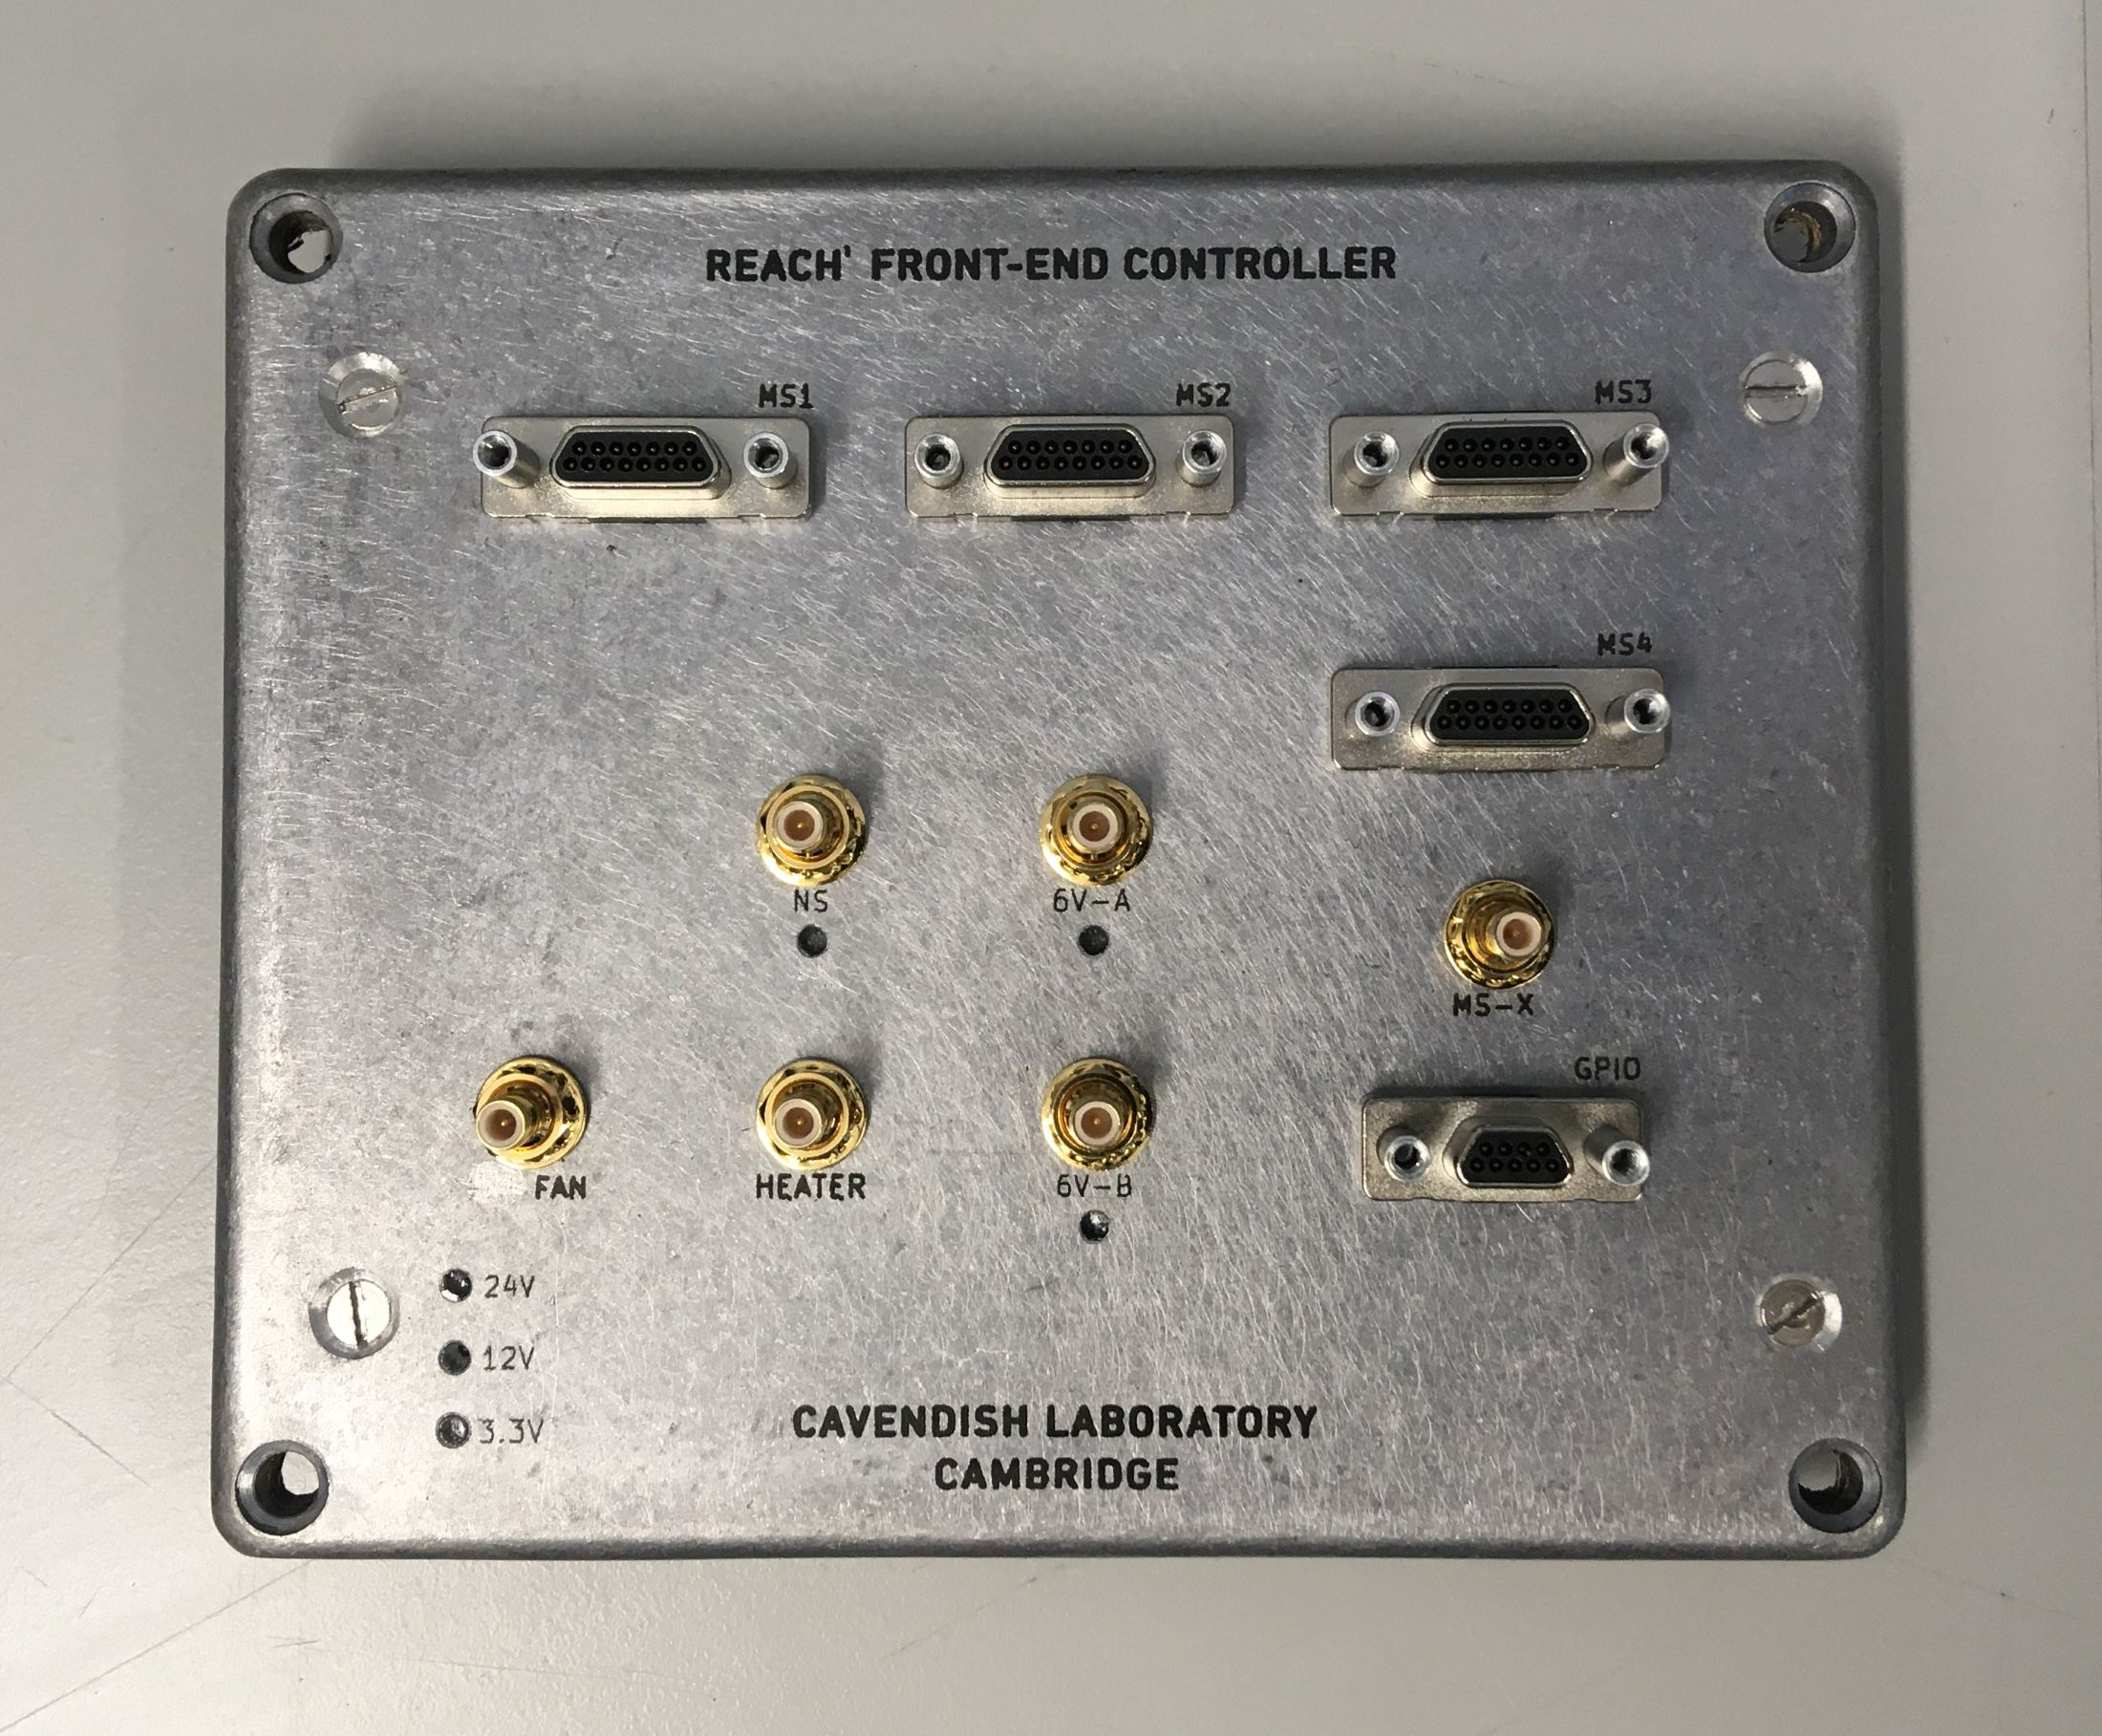
\includegraphics[width=\linewidth]{ucon_cover}
    \end{subfigure}
    \caption{The breakout board of the micocontoller is shown on the right displaying the mechanical switch connections across the top row. The remaining power supply connections can also be seen on the board. The top cover of the completed microcontoller unit is shown on the right with laser markings annotating the connections of the breakout board.}
    \label{fig:break_board}
\end{figure}
A CAD rendering depicting the stacked microcontroller unit is also shown as \cref{fig:ucon_cad}.
\begin{figure}
    \centering
    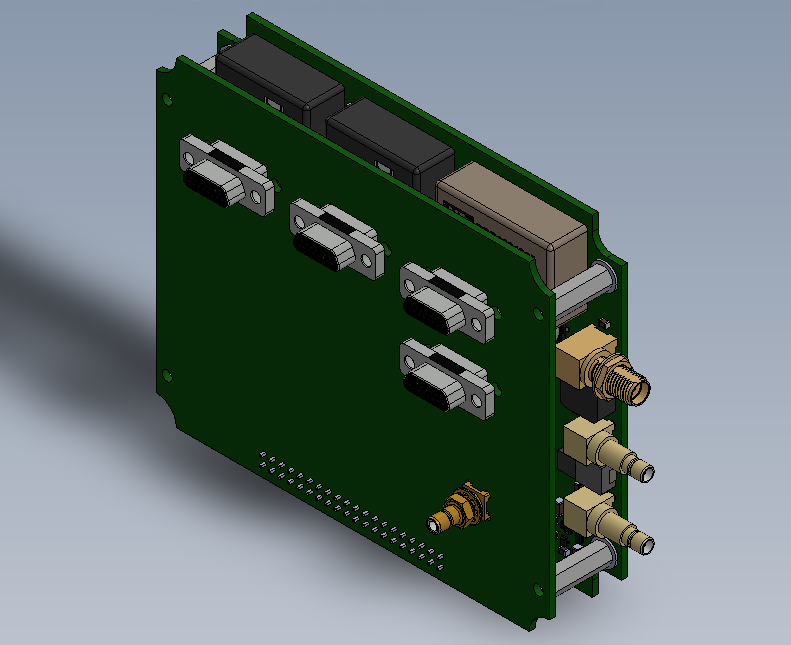
\includegraphics[scale=0.4]{stacked_ucon}
    \caption{A rendering of the micorcontroller assembly showing the breakout board seated above the controller board both outside the microcontroller housing. Also not shown is a heat transfer bracket between the three converter modules. The staked design of the microcontoller allowed for the small form factor required by the REACH experiment.}
    \label{fig:ucon_cad}
\end{figure}
The completed unit supplies power to every component within the front-end except for the thermal management system which has its own power supply unit as previously detailed. A combination of switched-mode power supply (SMPS) and linear regulators are employed to optimise both low noise and efficiency with the six DC-DC power supplies having an efficiency of at least 85\%. A table detailing the power supplies managed by the microcontroller unit is shown in \cref{tab:power_supply}. Further conductive gaskets were placed under bulkhead connectors for additional noise reduction and additional DC filtering is provided on the 48 V input supply. A block diagram of the completed microcontroller unit is provided in \cref{fig:ucon_block}.
\begin{figure}
    \centering
    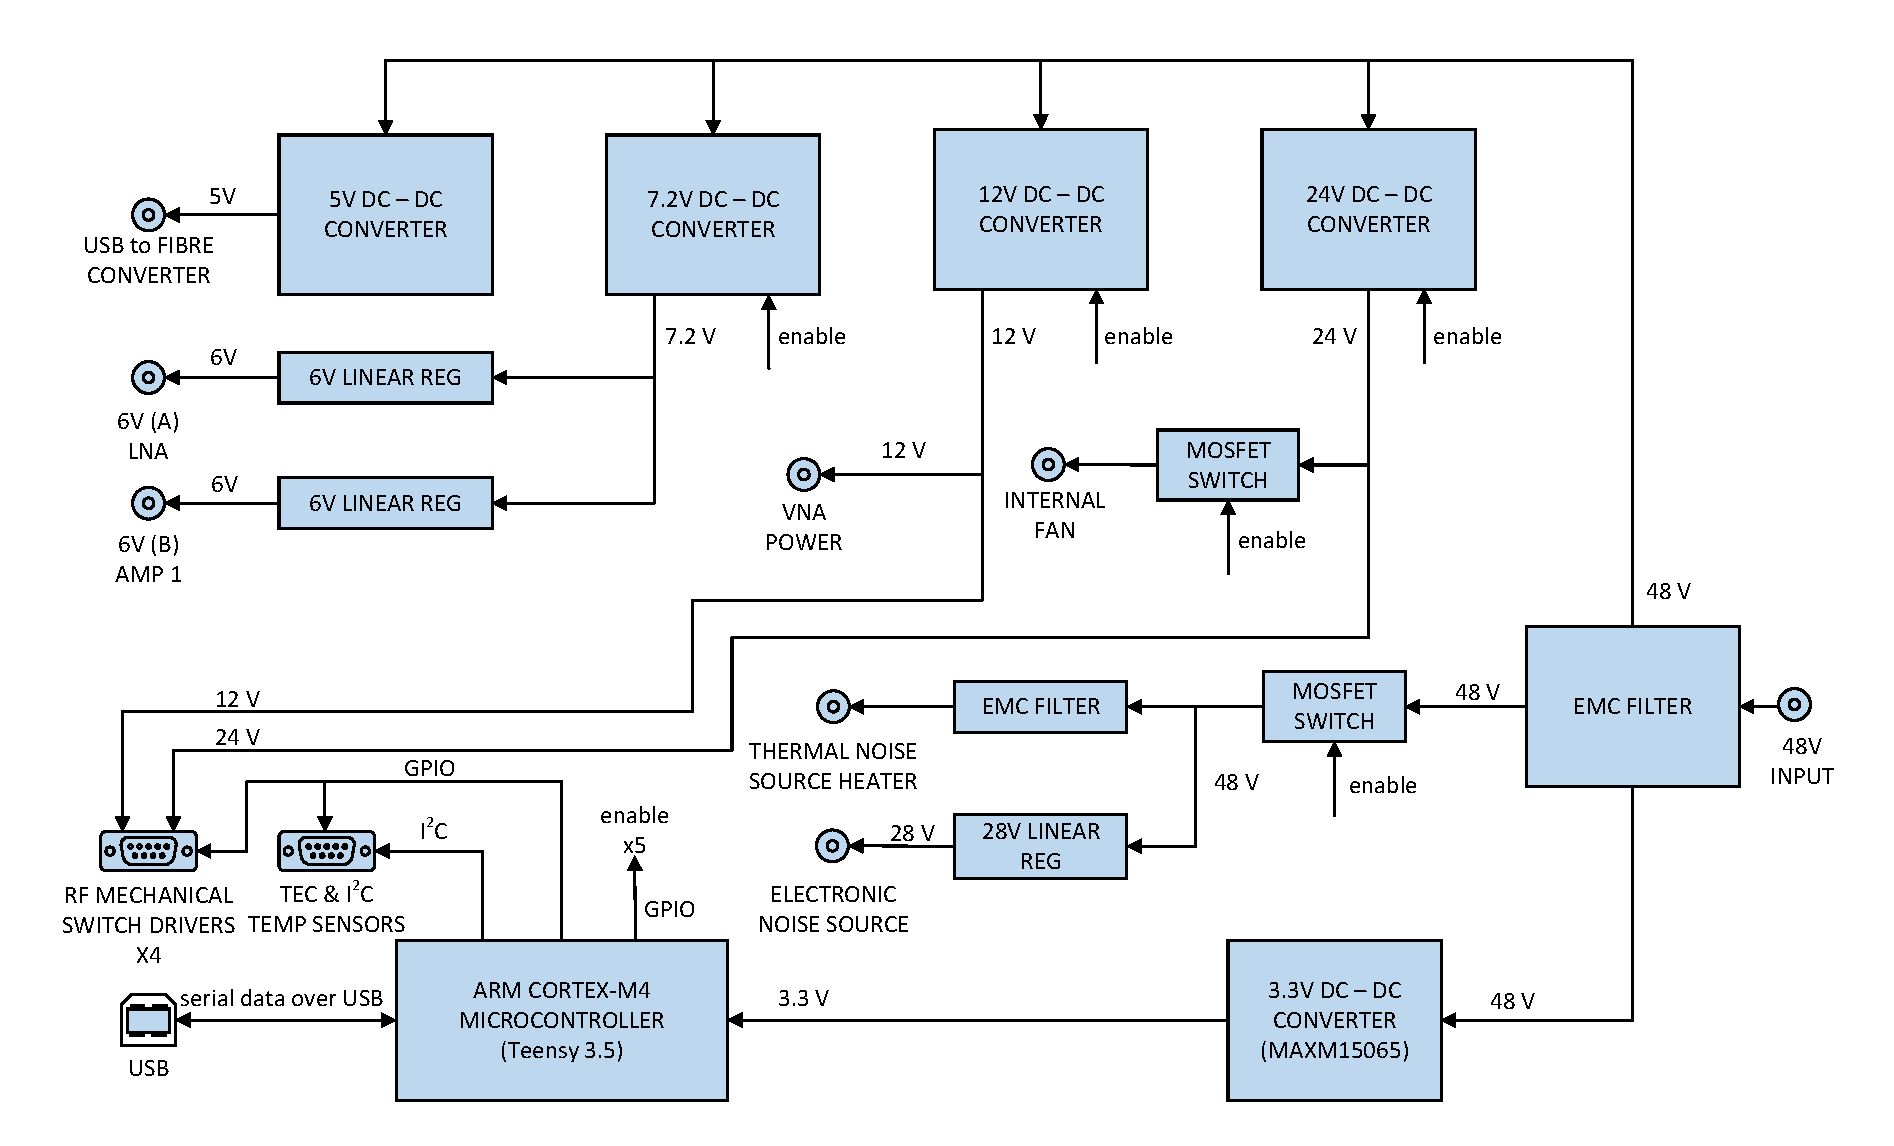
\includegraphics[width=\textwidth]{updated_controller_detail}
    \caption{A detailed microcontroller block diagram showing the components, connections and power considerations incorporated into the design.}
    \label{fig:ucon_block}
\end{figure}
The completed unit demonstrates a high efficiency with a 2 K temperature rise seen within the microcontroller casing with all supplies on at full load.


% =========================================
\subsubsection{Temperature measurement via thermocouple}
Within the receiver front-end are probes measuring the temperatures of various components needed for calibration. Initial designs utilised eight Microchip Technology MCP9808 temperature sensors that communicate directly with the microcontroller unit using I\textsuperscript{2}C protocol over the Arduino command line interface. Thermal gap pads would be used to thermally bond the 2-centimetre-wide temperature sensors to front-end components yielding an accuracy of $\pm 0.5$ K and measured with a cadence of I2C MEASUREMENT CADENCE HERE. The I\textsuperscript{2}C sensors’ native connection to the microcontroller unit conformed to the space restrictions of the front-end enclosure however, it was decided that smaller probe tips for placement on individual components as well as additional temperature sensors would increase the accuracy of our calibration prescription. A Pico Technology TC-08 Thermocouple Data Logger, shown in \cref{fig:tc08}, was employed to accommodate eight more temperature measurements using Pico Technology SE000 K-type thermocouples with TC-08 0.60 mm tip ends thermally bonded to components using RTV Thermally Conductive Oxime made by Electrolube.
\begin{figure}
    \centering
    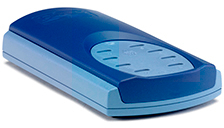
\includegraphics[width=0.4\textwidth]{tc08}
    \caption{The Pico Technology TC-08 Thermocouple Data Logger for use with eight K-type thermal probes.}
    \label{fig:tc08}
\end{figure}
The simple incorporation of the TC-08 with our receiver automation software through the manufacturer’s proprietary Python libraries also factored into our decision to use the device. The TC-08 thermocouples have an accuracy of $\pm 1.1$ K\footnote{Sum of $\pm0.2$\% of reading and $\pm0.5$ K according to manufacturer specifications.} for our measurements typically around 300 K and relay information to the back-end server via USB connection at a cadence of one measurement every 10 seconds. A table of the TC-08 Data Logger port assignments is shown in \cref{tab:tc08}\footnote{These port assignments are representative of the front-end configuration at the time of shipment to South Africa in December 2022 and are subject to change.}.
\begin{table}
    \begin{center}
    \begin{tabular}{ |c|c| }
    \hline
    TC-08 Port Number & Component \\
    \hline
    Port 0 & Cold Junction \\
    Port 1 & MS1 switch \\
    Port 2 & Heated load thermistor \\
    Port 3 & MS3 switch\\
    Port 4 & MS4 switch \\
    Port 5 & 2 metre calibration cable \\
    Port 6 & 10 metre calibration cable \\
    Port 7 & Low noise amplifier \\
    Port 8 & Antenna (laboratory) \\
    \hline
    \end{tabular}
    \caption{The port assignments for the TC-08 connecting to various components within the receiver front-end. The Port 2 thermocouple was attached to the thermistor end of the simplified heated load construction. The Port 5 and 6 probes were connected directly to the outside of the calibration cables for measurement of the physical cable temperature with the terminating sources assumed to be at the same temperature as their respective switches. In the Cambridge laboratory, the Port 8 thermocouple was fed through a small hole drilled through the wall of the front-end enclosure and attached to the end of a makeshift antenna used for testing of the calibration algorithm.}
    \label{tab:tc08}
    \end{center}
\end{table}

We highlight that Port 0 of the TC-08 lists a “Cold Junction” which is the temperature of the Data Logger unit itself and not the similarly named ambient temperature “cold” load. Furthermore, the position of the MCP9808 I\textsuperscript{2}C temperature sensors were not finalised or thermally bound to anything by the time of deployment in August 2023 though it is envisioned that measurements of additional components needed for the temperature corrections detailed in TEMPERATURE CORRECTIONS CHAPTER are the primary responsibility of the I\textsuperscript{2}C sensors. The temperature stability of various sources recorded by the TC-08 are shown in \cref{fig:temperature}.
\begin{figure}
    \centering
    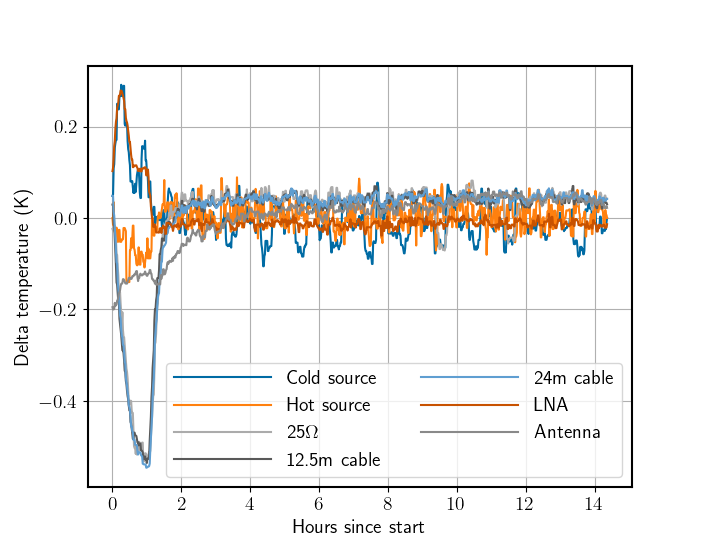
\includegraphics[scale=0.6]{temperature}
    \caption{Receiver component temperature stability recorded by the TC-08 Data Logger. The fluctuations seen within the first two hours of the measurements are from mechanical switch stabilisation and the VNA calibration procedure. We highlight the temperature stability of the individual components after environmental stability is achieved. The plot includes measurements of the 12.5 metre and 24 metre calibration cables before being replaced by the 2 metre and 10 metre cables as detailed in Calibration sources subsection.}
    \label{fig:temperature}
\end{figure}


% =========================================
\subsubsection{Vector Network Analyser}
Reflection coefficients of the calibration sources, LNA and antenna are measured with a Copper Mountain Technologies TR1300/1 2-port 1.3 GHz vector network analyser (VNA) shown in \cref{fig:vna}.
\begin{figure}
    \centering
    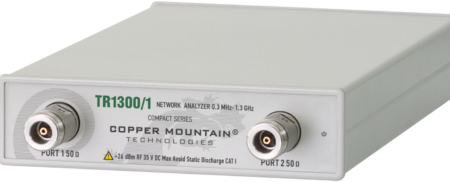
\includegraphics[scale=0.5]{vna}
    \caption{Copper Mountain Technologies TR1300/1 Vector Network Analyser. Image taken from Copper Mountain Technologies website.}
    \label{fig:vna}
\end{figure}
The main consideration for including this VNA model was the small $28.5 \times 14.2 \times 4$ cm form factor for inclusion in the front-end enclosure. The VNA measurement accuracy as provided by the manufacturer is shown in \cref{tab:vna_acc}.
\begin{table}
    \begin{center}
    \begin{tabular}{ |c|c| }
    \hline
    Reflection measurement & Accuracy (Magnitude) \\
    \hline
    -15 dB to 0 dB & $\pm$0.4 dB \\
    -25 dB to -15 dB & $\pm$1.5 dB \\
    -35 dB to -25 dB & $\pm$4.0 dB \\
    \hline
    \end{tabular}
    \caption{Manufacturer quoted measurement accuracies for the Copper Mountain Technologies TR1300/1 Vector Network Analyser.}
    \label{tab:vna_acc}
    \end{center}
\end{table}

Reflection coefficient measurements of various receiver components is shown in \cref{fig:s11_meas}. 
\begin{figure}
    \centering
    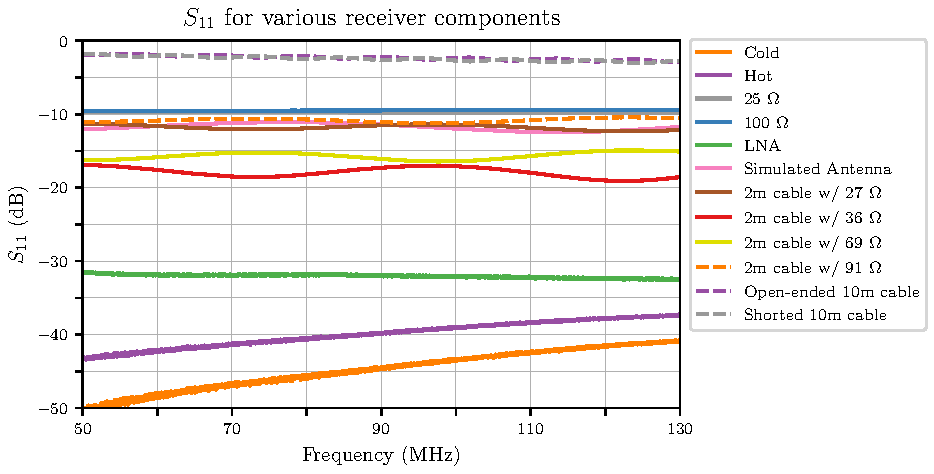
\includegraphics[width=\columnwidth]{s11_meas}
    \caption{Reflection coefficients for various receiver components including the LNA and simulated antenna.}
    \label{fig:s11_meas}
\end{figure}
Upon inspection of \cref{tab:vna_acc}, one may note that the VNA is not rated for extremely low reflection measurements below -35 dB such as the ambient temperature and heated $50\Omega$ loads shown in \cref{fig:s11_meas}. In order to quantify the quality of our measurements in this low-reflection regime, we use the manufacturer provided data of \cref{tab:vna_acc} and calculate a spread in $\pm$dBs representing our measurement error for the regions our machine is rated for. We then convert this spread from dB to linear using
\begin{equation}
    \mathrm{measurement \ spread} = 10^{\frac{\mathrm{measurement} + \mathrm{error}}{10}} - 10^{\frac{\mathrm{measurement} - \mathrm{error}}{10}}
    \label{eq:vna_spread}
\end{equation}
The linear measurement spreads are plotted in \cref{fig:vna_acc} where we have fitted the manufacturer provided data with a decaying exponential using \textsc{SciPy.optimize} and extrapolated to the ranges applicable to the 50$\Omega$ loads. \begin{figure}
    \centering
    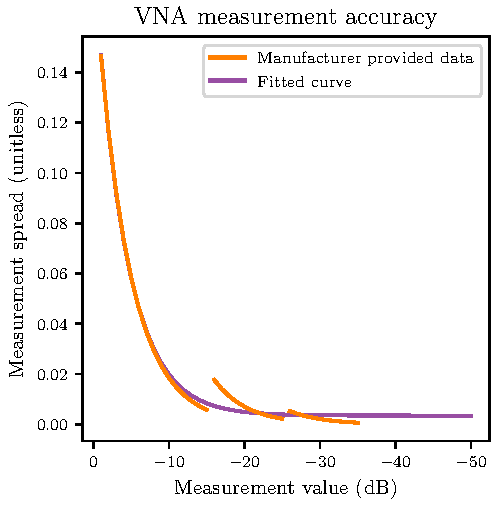
\includegraphics{linear_vna_accuracy}
    \caption{VNA measurement spreads on a linear scale as a fraction of reflected power representing the measurement accuracy of the machine. Manufacturer provided data are shown in orange. A best-fit exponential curve to the manufacturer data is plotted in purple. The fitted curve asymptotes at a value of 0.002.}
    \label{fig:vna_acc}
\end{figure}
For reflection coefficient measurements $\sim -45$ dB, we find a linear measurement spread of 0.002 corresponding to a VNA accuray of $\pm$10 dB. In the logarithmic scale of dBs, this measurement accuracy is acceptable. A similar exercise of fitting a polynomial curve to the manufacturer provided data in the dB scale gives a similar but less conservative value for extrapolated measurement accuracy. We note that future iterations of the receiver front-end may benefit from inclusion of a VNA rated for low-reflection measurements but the small form factor of the TR1300/1 may be difficult to achieve.

A Python script using SCPI commands was developed in order to interact with and automate the VNA. This included a separate process to calibrate the VNA itself before proceeding with calibration of the receiver. VNA calibration was undertaken using short, open and load (SOL) standards from another Kirkby 85033 50$\Omega$ SMA calibration kit to maximise measurement accuracy of the reflection coefficients throughout a 50–-200 MHz band. The VNA calibration is tested against an additional $50\Omega$ test load that was measured in Cambridge with a Keysight N5247A PNA-X Network Analyser capable of providing some of the highest quality reflection measurements in the industry\footnote{The 49 kg PNA-X, with a size of $649 \times 482 \times 280$ mm, unfortunately proves to be too large for in-field deployment.}. A reflection coefficient of the test load measured by the TR1300/1 that deviates from the PNA-X measurement by more than 5\% automatically triggers a re-calibration of the VNA before proceeding with calibration of the rest of the instrument.


% =========================================
\subsubsection{USB-over-fibre connection}
As briefly indicated in previous sections, the relay of instructions and measurement data from front-end components such as the TEC control module, microcontroller unit, TC-08 and VNA requires a USB connection to the satellite-linked server housed 100 metres away in the receiver back-end. To avoid RFI, signal loss or the logistical issues of constructing 100-metre-long shielding for a series of USB cable extenders, a 4-port Icron 2244 USB Ranger\footnote{As this model is now a legacy device, the Icron 2344 USB Ranger is expected to be used for any future receiver builds.} is used to convert USB data into fibre optical signals for transmission between the two nodes at up to 480 Mbps. Opting to mitigate any potential impact of distance-dependent signal dispersion or degradation, a phenomenon commonly observed in multi-mode fibre optic connections spanning over 500 metres, single-mode fibre optical connections were specifically chosen to ensure signal preservation despite the relatively short distance of 100 metres. Powered by the microcontroller unit, the 5 V USB Ranger is held in place by a custom 3D printed bracket and outputs through a single-mode fibre port installed on the front-end enclosure as labelled in \cref{fig:enclosure_external_connections}.


% =========================================
\subsubsection{RF signal chain I: Low noise amplifier}
Cosmic radio signals detected by the antenna are generally weak and need to be amplified to measurable levels. Because random electrical noise from instrumental components would also be magnified by across-the-board amplification, several stages of low-level, more precise amplification are needed to preserve any celestial signatures. The primary ‘preamplification’ stage of the RF signal chain is commonly managed by a ‘Low Noise Amplifier’ (LNA) which is tasked with amplifying incoming signals while adding a minimal amount of noise. 

An inspection of typical noise figure circles from RF transistor datasheets indicate a general trade-off between maximal noise figure and perfect impedance matching. For REACH, we have opted to prioritise impedance matching in our design to minimise reflections producing the noise waves necessitating calibration. The resulting LNA is therefore not particularly low-noise, but this is anticipated to have a negligible impact on the REACH experiment due to long integration times serving to counteract sensitivity limitations. It is expected that the REACH system will be sky noise dominated in the 60--120 MHz regime where the dipole is best matched with reduced sensitivity at frequencies greater than 120 MHz.

With the design objectives of an amplifier input reflection coefficient (S\textsubscript{11}) less than -30 dB as well as a low gain variation with temperature, several amplifiers were assessed before ultimately selecting a pair of Mini-Circuits CMA-84+ SMT gain blocks followed by attenuators to realise an exceptional input matching along with a spectrally flat passband response. The completed LNA, shown in \cref{fig:lna} ultimately achieves a flat 5.1 dB noise figure within the REACH observational band of 50--170 MHz.
\begin{figure}
    \centering
    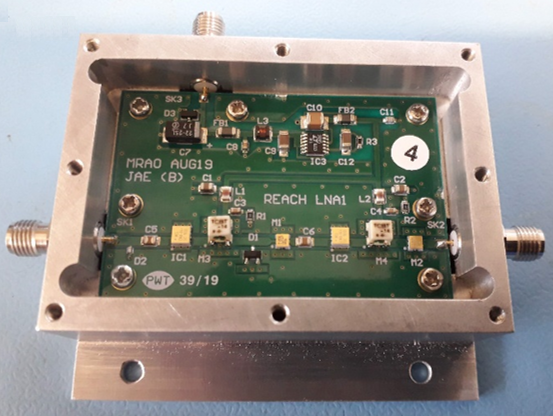
\includegraphics[scale=0.5]{lna}
    \caption{Interior of the completed REACH low noise amplifier custom designed for a flat spectral response in both S\textsubscript{11} and noise.}
    \label{fig:lna}
\end{figure}

While an alternative LNA built instead with Mini-Circuits ERA-50SM+ gain blocks exhibited a better noise figure of 3.3 dB, the CMA-84+ construction demonstrated a better stability in both S\textsubscript{11} and temperature. Reflection coefficients of the finalised LNA are plotted in \cref{fig:lna_sparams} showing the desired S\textsubscript{11} less than -30 dB which is well matched across the observational band as well as a remarkably flat 40 dB gain response.
\begin{figure}
    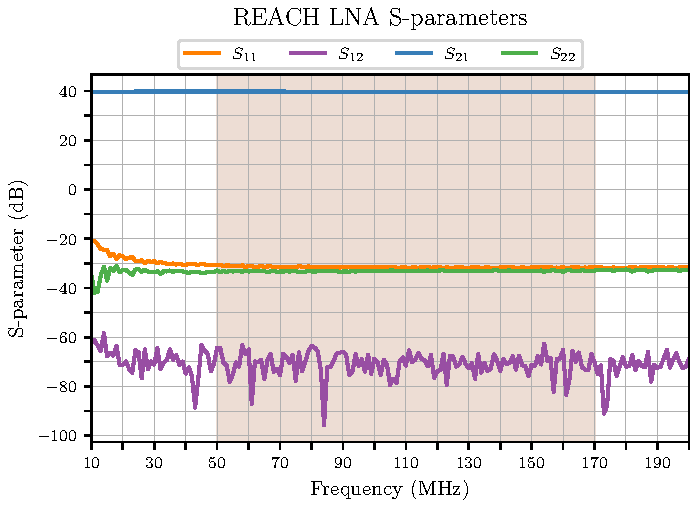
\includegraphics[width=\columnwidth]{lna_sparams}
    \caption{Measured S-parameters of the REACH LNA showing a good match at -30 dB for the $S_{11}$ and $S_{22}$ across the REACH observation band (shaded region) while demonstrating exceptional gain stability ($S_{21}$).}
    \label{fig:lna_sparams}
\end{figure}


% =========================================
\subsubsection{RF signal chain II: Amplifier \#1}
The second stage of spectral data amplification uses another custom module called ‘Amplifier \#1’, or AMP1\footnote{Like all good computer scientists, we have numbered our amplifiers using a zero-based system with the LNA, AMP1 and AMP2 being amplifiers number zero, one and two respectively in the RF signal chain.}. Incoming signals from the LNA are further amplified using a Mini-Circuits GALI-S66+ limiting amplifier and a PHA-13LN+ mid-power amplifier in combination to achieve maximal dynamic range followed by high-pass filtering using a Mini-Circuits RHP-44+ filter to attenuate frequencies below the observation band. A 2-stage Mini-Circuits XLF-42M+ monolithic microwave integrated circuit (MMIC) then low-pass filters out-of-band signals above the observation band up to many GHz.

Serving as the internal circuit boundary of the front-end receiver, AMP1 converts signals to Radio-Frequency-over-Fibre for transmission to the receiver back-end minimising the effects of RFI and signal loss that would be typical of alternative connections such as coaxial cables. The passive 1310 nm RFoF converter was made under commission by Polycom according to the specifications for the HERA experiment and has an 18 dB loss due the relative intensity noise of the optical transmission laser which is addressed by 70 dB of upfront gain to reduce the impact of higher noise on the system. The optical transmitter subassembly (as well as the corresponding back-end optical receiver) are printed circuit boards terminated in Fibre Channel/Angled Physical Contact (FC/APC) connectors at the end of a 0.5 metre pigtail as seen in \cref{fig:amp1}.
\begin{figure}
    \centering
    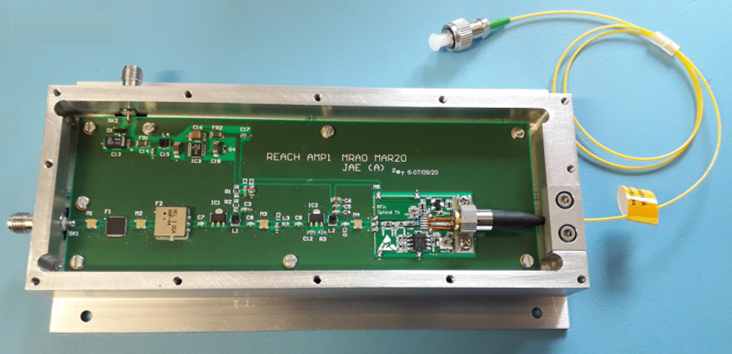
\includegraphics[scale=0.5]{amp1}
    \caption{The REACH AMP1 module used for further amplification and filtering of signals. Seen on the right end of the construction is the fibre optic conversion printed circuit board connected to the single-mode FC/APC RFoF transmission connector seen in yellow.}
    \label{fig:amp1}
\end{figure}
The FC/APC connector links to the RFoF port installed on the front-end enclosure as labelled in \cref{fig:enclosure_external_connections} which connects to an extended roll of fibre optical cabling reaching the receiver back-end. Single-mode fibre optics are again used to prevent signal degradation as with the USB-over-fibre connection. We find the radio-frequency loss of the RFoF bridge over the 100 metre distance to be less than 1 dB including the connections at both ends. A full circuit diagram of amplifier \#1 including the RFoF transducer is shown in \cref{fig:amp1_schematic}.


% =========================================
\subsubsection{Completed receiver front-end unit}
The deployable receiver front-end unit was completed in December 2022 and is shown in \cref{fig:frontend_complete}. 
\begin{figure}
    \centering
    \centering
    \begin{subfigure}{.45\textwidth}
        \centering
        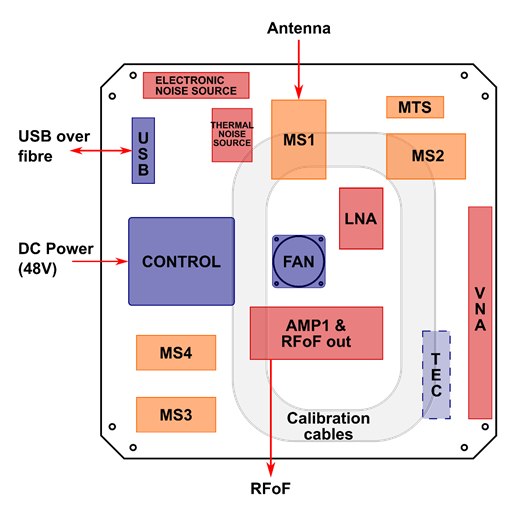
\includegraphics[width=\linewidth]{frontend_layout}
    \end{subfigure}
    \hfill
    \begin{subfigure}{.45\textwidth}
    \centering
        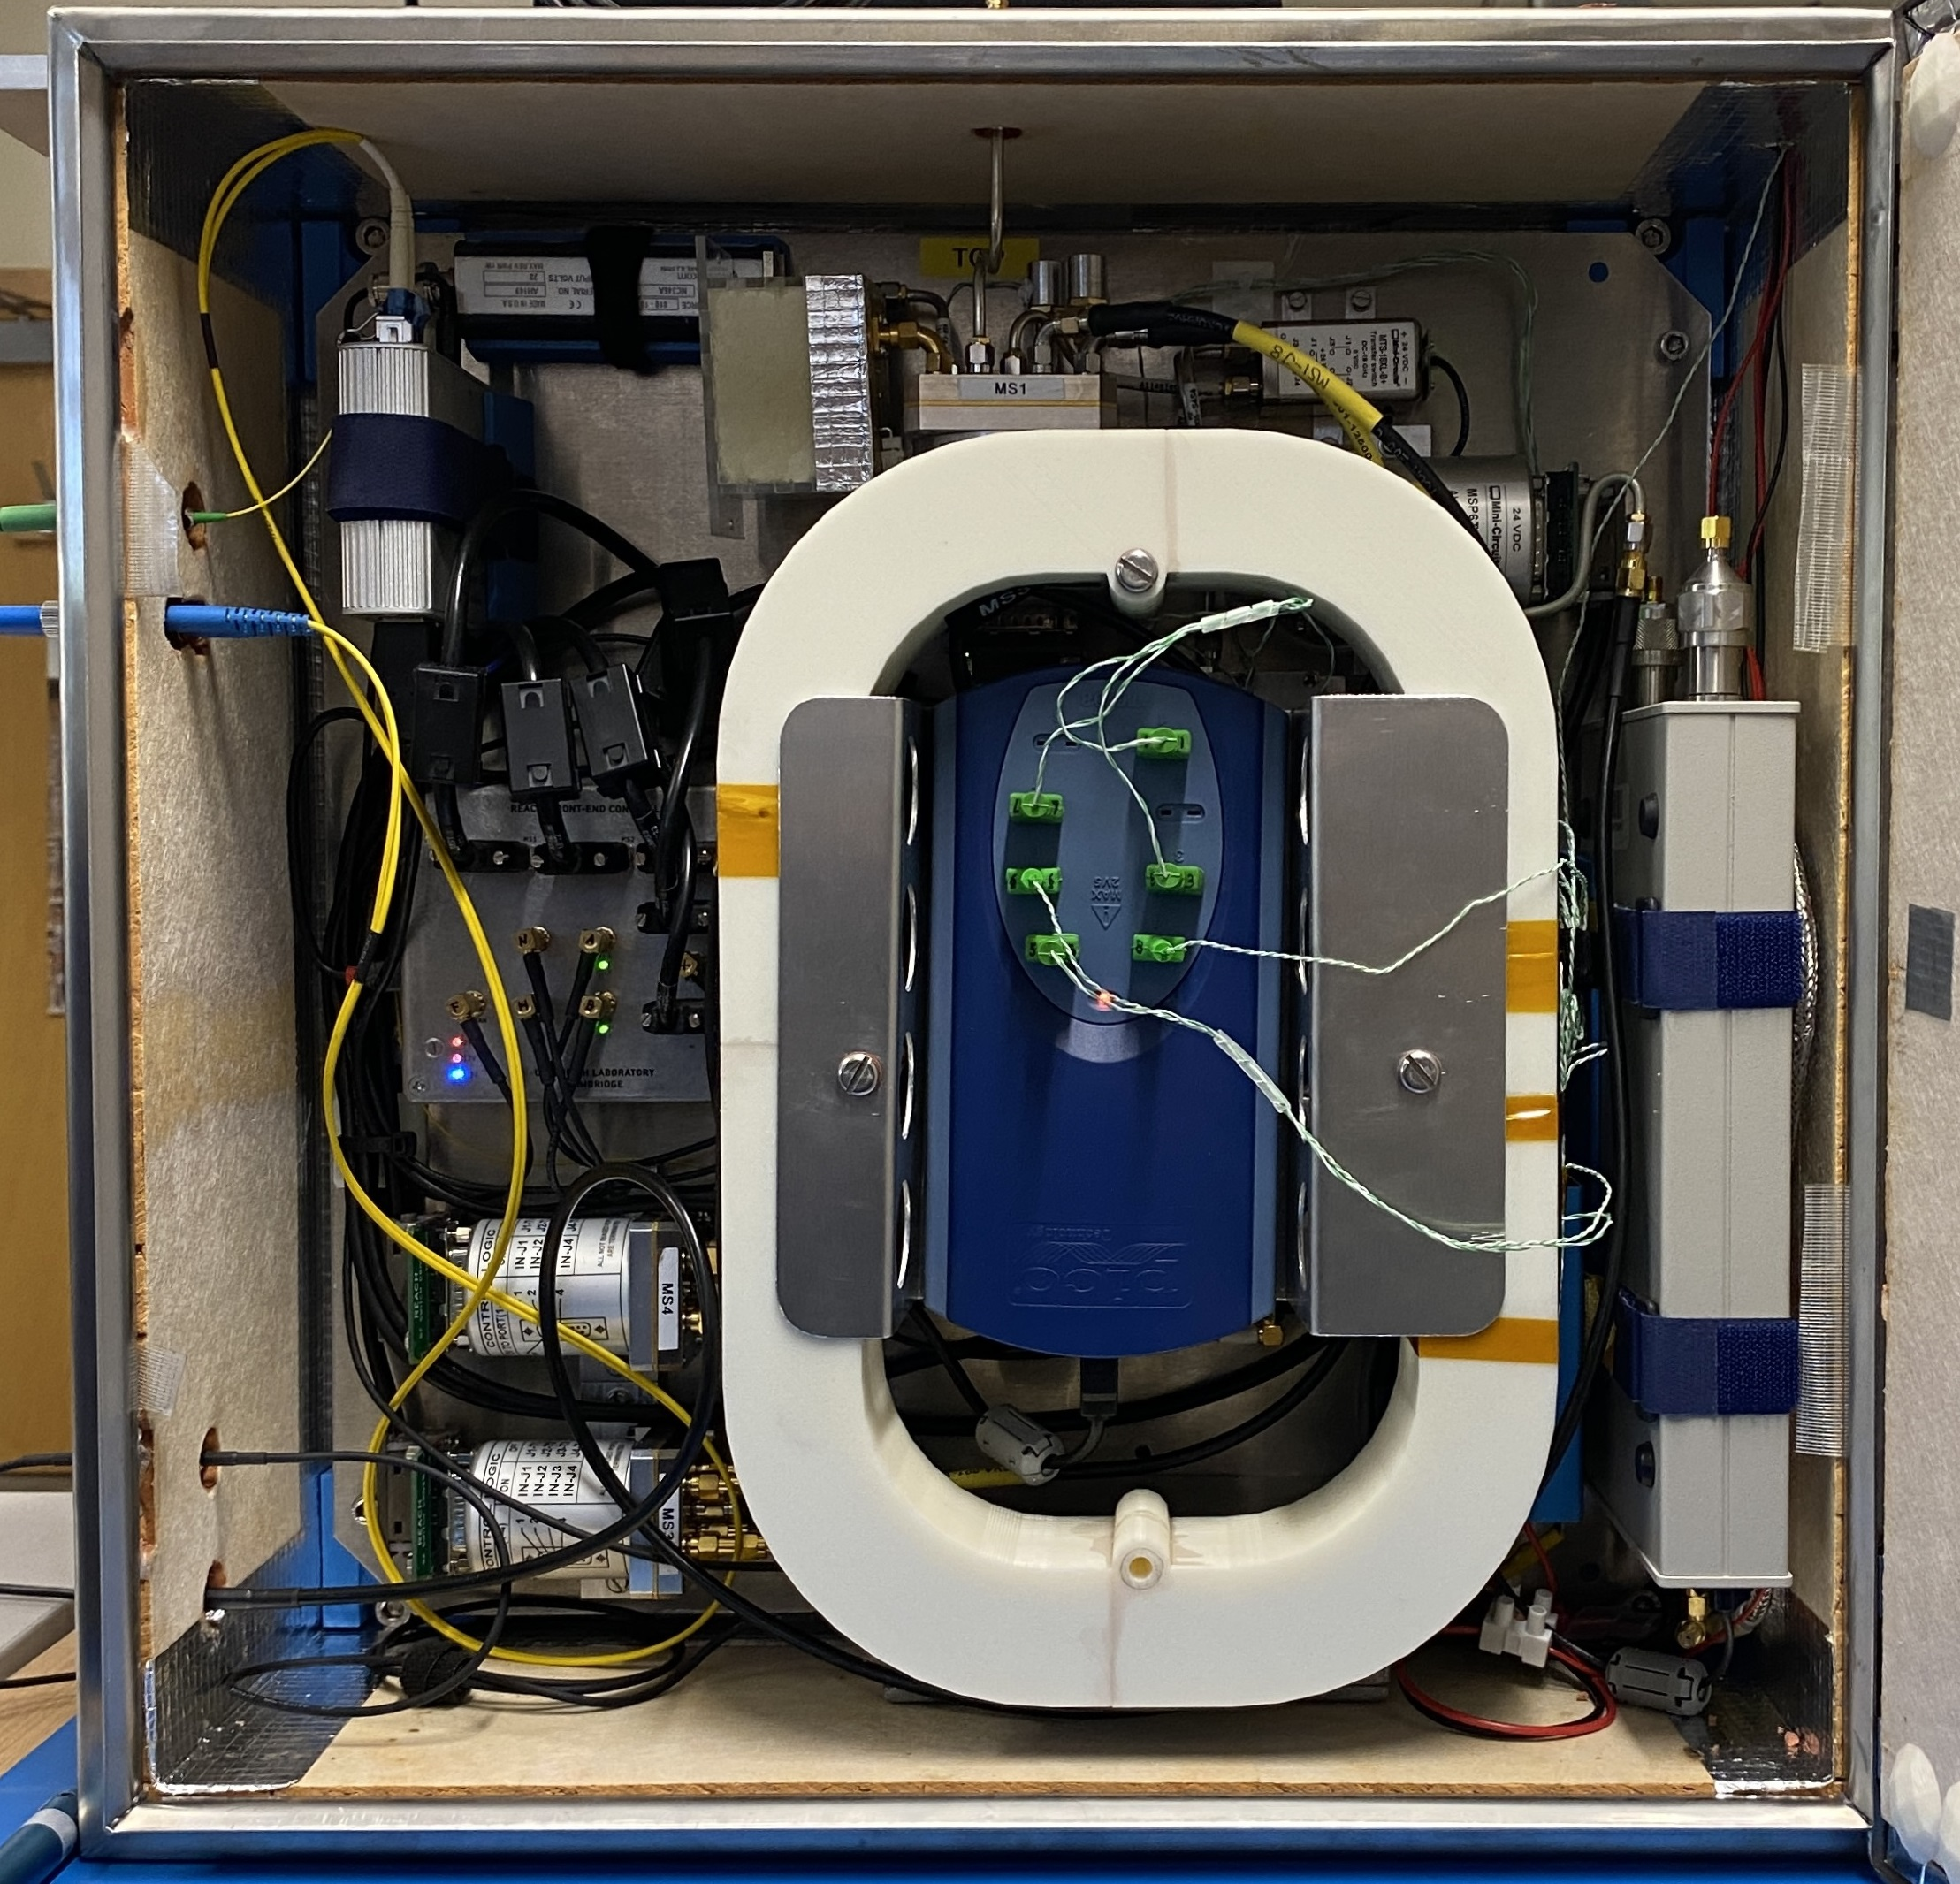
\includegraphics[width=\linewidth]{frontend.jpeg}
    \end{subfigure}
    \caption{The completed receiver front-end unit (right) along with a layout diagram showing the approximate positions of various components (left). Shown in the image are the compact VNA on the bottom right and the TC-08 module in the centre with green thermocouple probes. The stadium housing the calibration cables is seen around the TC-08 and obscures the amplifiers and TEC. The various cylinders are the multi-input switches connected to calibration sources. The microcontroller unit can be seen on the middle-left and is powered on as shown by the LED's. The USB over fibre link and diode noise source are shown in the top left corner.}
    \label{fig:frontend_complete}
\end{figure}
The finalised construction weighs 29 kilograms and, as stated previously, is allocated a maximum of 135 W for total front-end power from the solar panels. Control and RF circuitry require about 31.5 W with the remaining 103.5 W left for cooling through the TEC. The majority of the engineering work went in to construction of this receiver front-end and is expected to be deployed as a portable, energy efficient system with accurate in situ calibration through internal environmental control while maintaining the highest quality measurement capabilities and RFI mitigation. Also included are various ferrite beads to limit control and power signals from intercepting the RF singal path and were generally placed through trial-and-error. Subcomponents along the signal chain are connected with RG-402 semi-rigid cables to prevent cable flexing during transportation. A second 1:1 replica of the receiver is currently being built in Cambridge to assist in remote triage expected during deployment and design changes are being considered for future front-ends to accommodate additional antennas. A picture of the receiver front-end deployed on the REACH site in South Africa is shown in \cref{fig:frontend_deployed}.
\begin{figure}
    \centering
    \includegraphics[scale=0.5]{example-image-c}
    \caption{The receiver front-end in its natural environment, deployed at the REACH experiment site in the Karoo Radio Astronomy Reserve, South Africa.}
    \label{fig:frontend_deployed}
\end{figure}


% =========================================
\subsection{Receiver back-end}\label{sec:backend}
The receiver back-end houses the components critical for remote communication away from the deployment site, power distribution to the instrument as a whole and measurement subsystems that are less sensitive to environmental effects. 100 metres away from the dipole antenna, the receiver back-end sits below ten MODEL NUMBERS solar panels rated to give SPECIFICATIONS HERE as diagrammed in \cref{fig:system_diagram}. This distance was chosen to avoid radio-frequency reflections off the solar panel and back-end faces as well as serving as a potential central node to be equidistant from future antennas. Under the solar panel construction is a radio-frequency electromagnetic-compatibility (RF-EMC) enclosure custom made by Interference Testing and Consultancy Services Ltd. to mitigate the effects of external RFI on our measurements as well as any potential EMI leakage from our own instrument that may be picked up by nearby experiments. Designs for the RF-EMC enclosure were informed by similar constructions used with the HERA experiment that incorporate considerations of the on-site environment as well as compliance with the EMC requirements of the Karoo Radio Astronomy Reserve. A conceptual diagram of the RF-EMC enclosure is shown in \cref{fig:backend}.
\begin{figure}
    \centering
    \centering
    \begin{subfigure}{.45\textwidth}
        \centering
        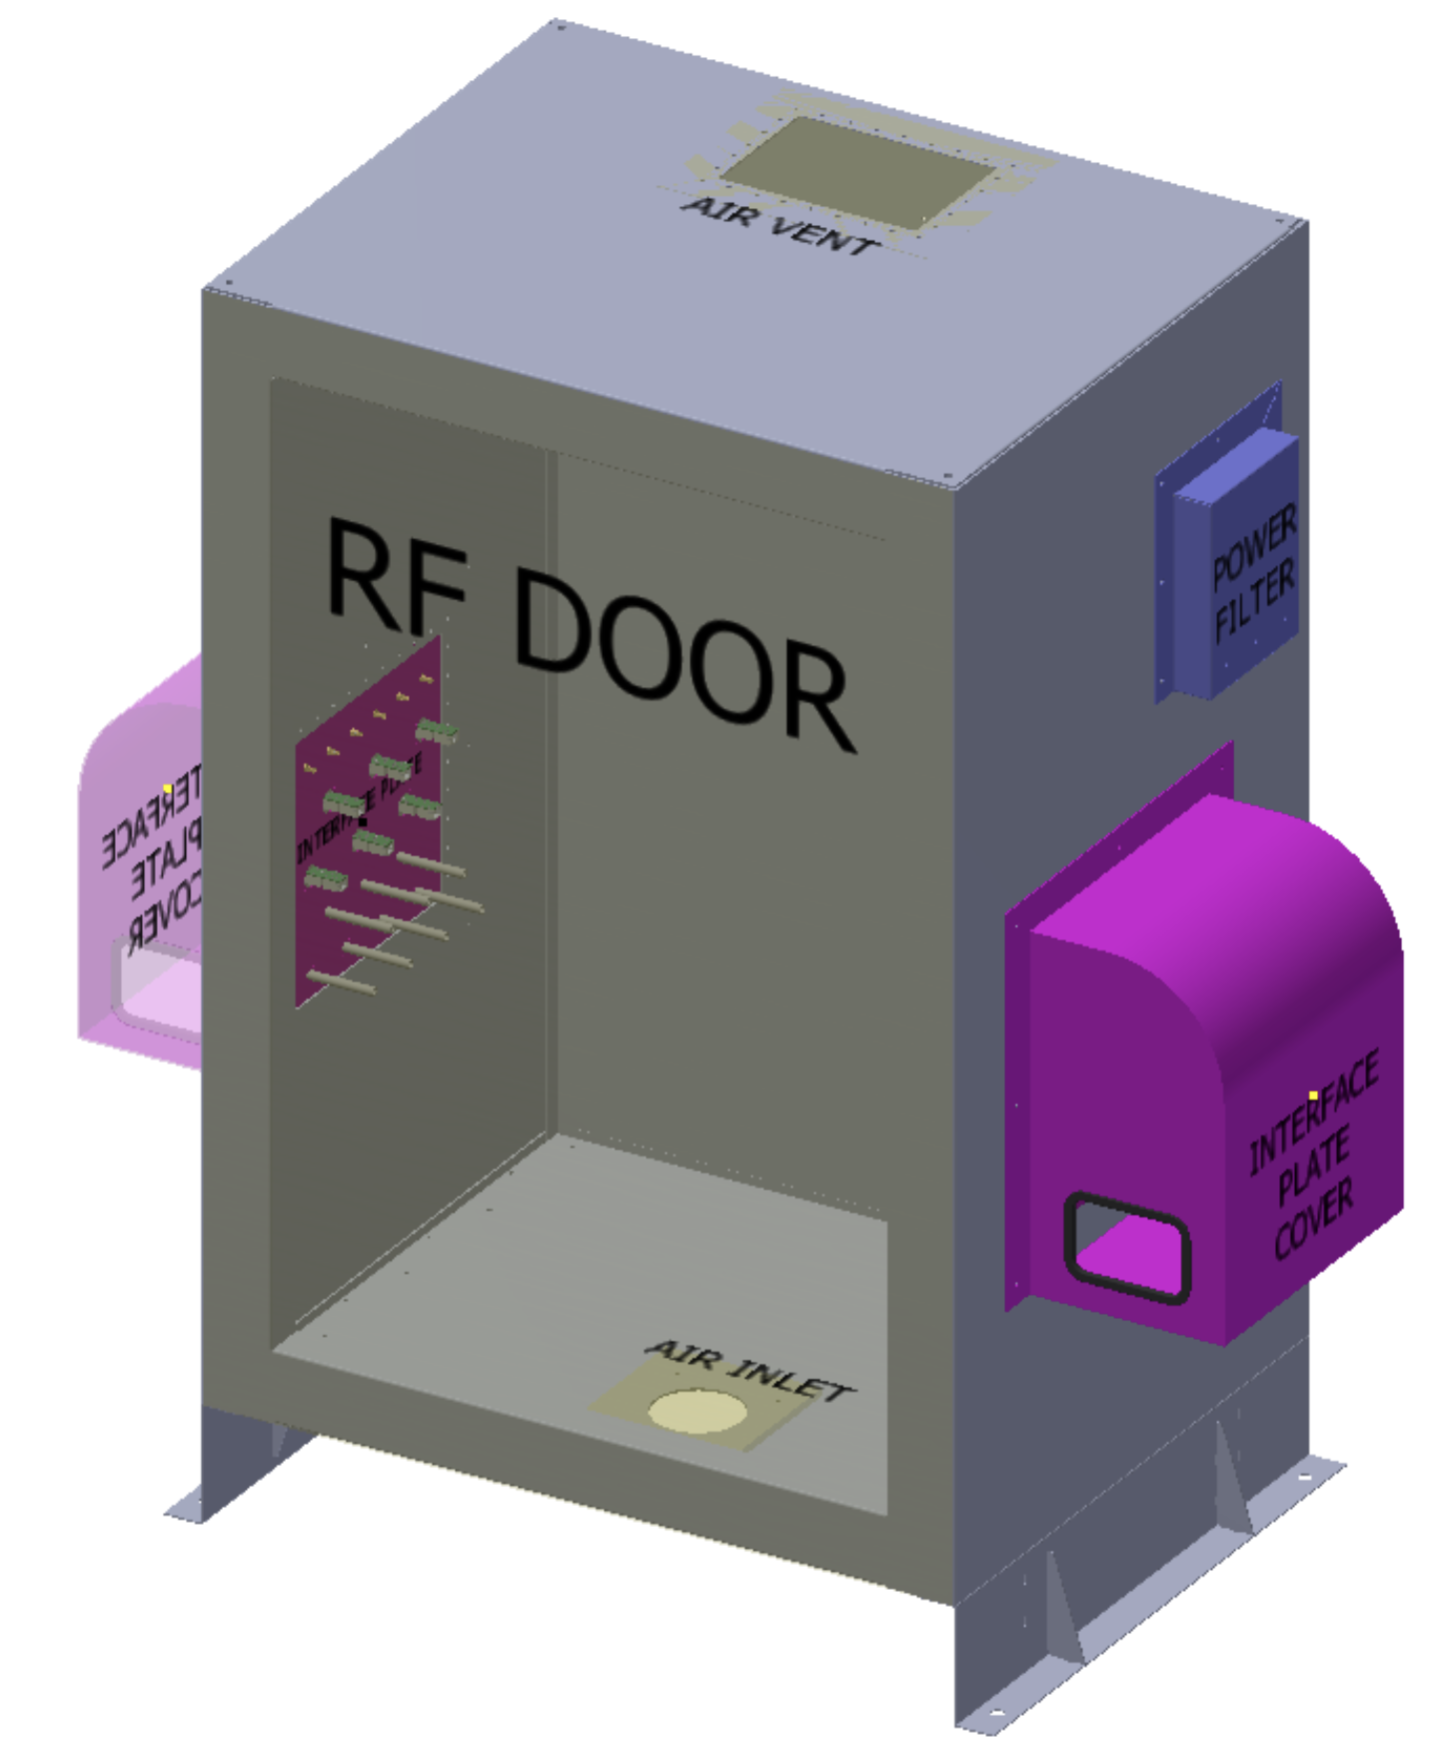
\includegraphics[width=\linewidth]{backend_diag}
    \end{subfigure}
    \hfill
    \begin{subfigure}{.4\textwidth}
    \centering
        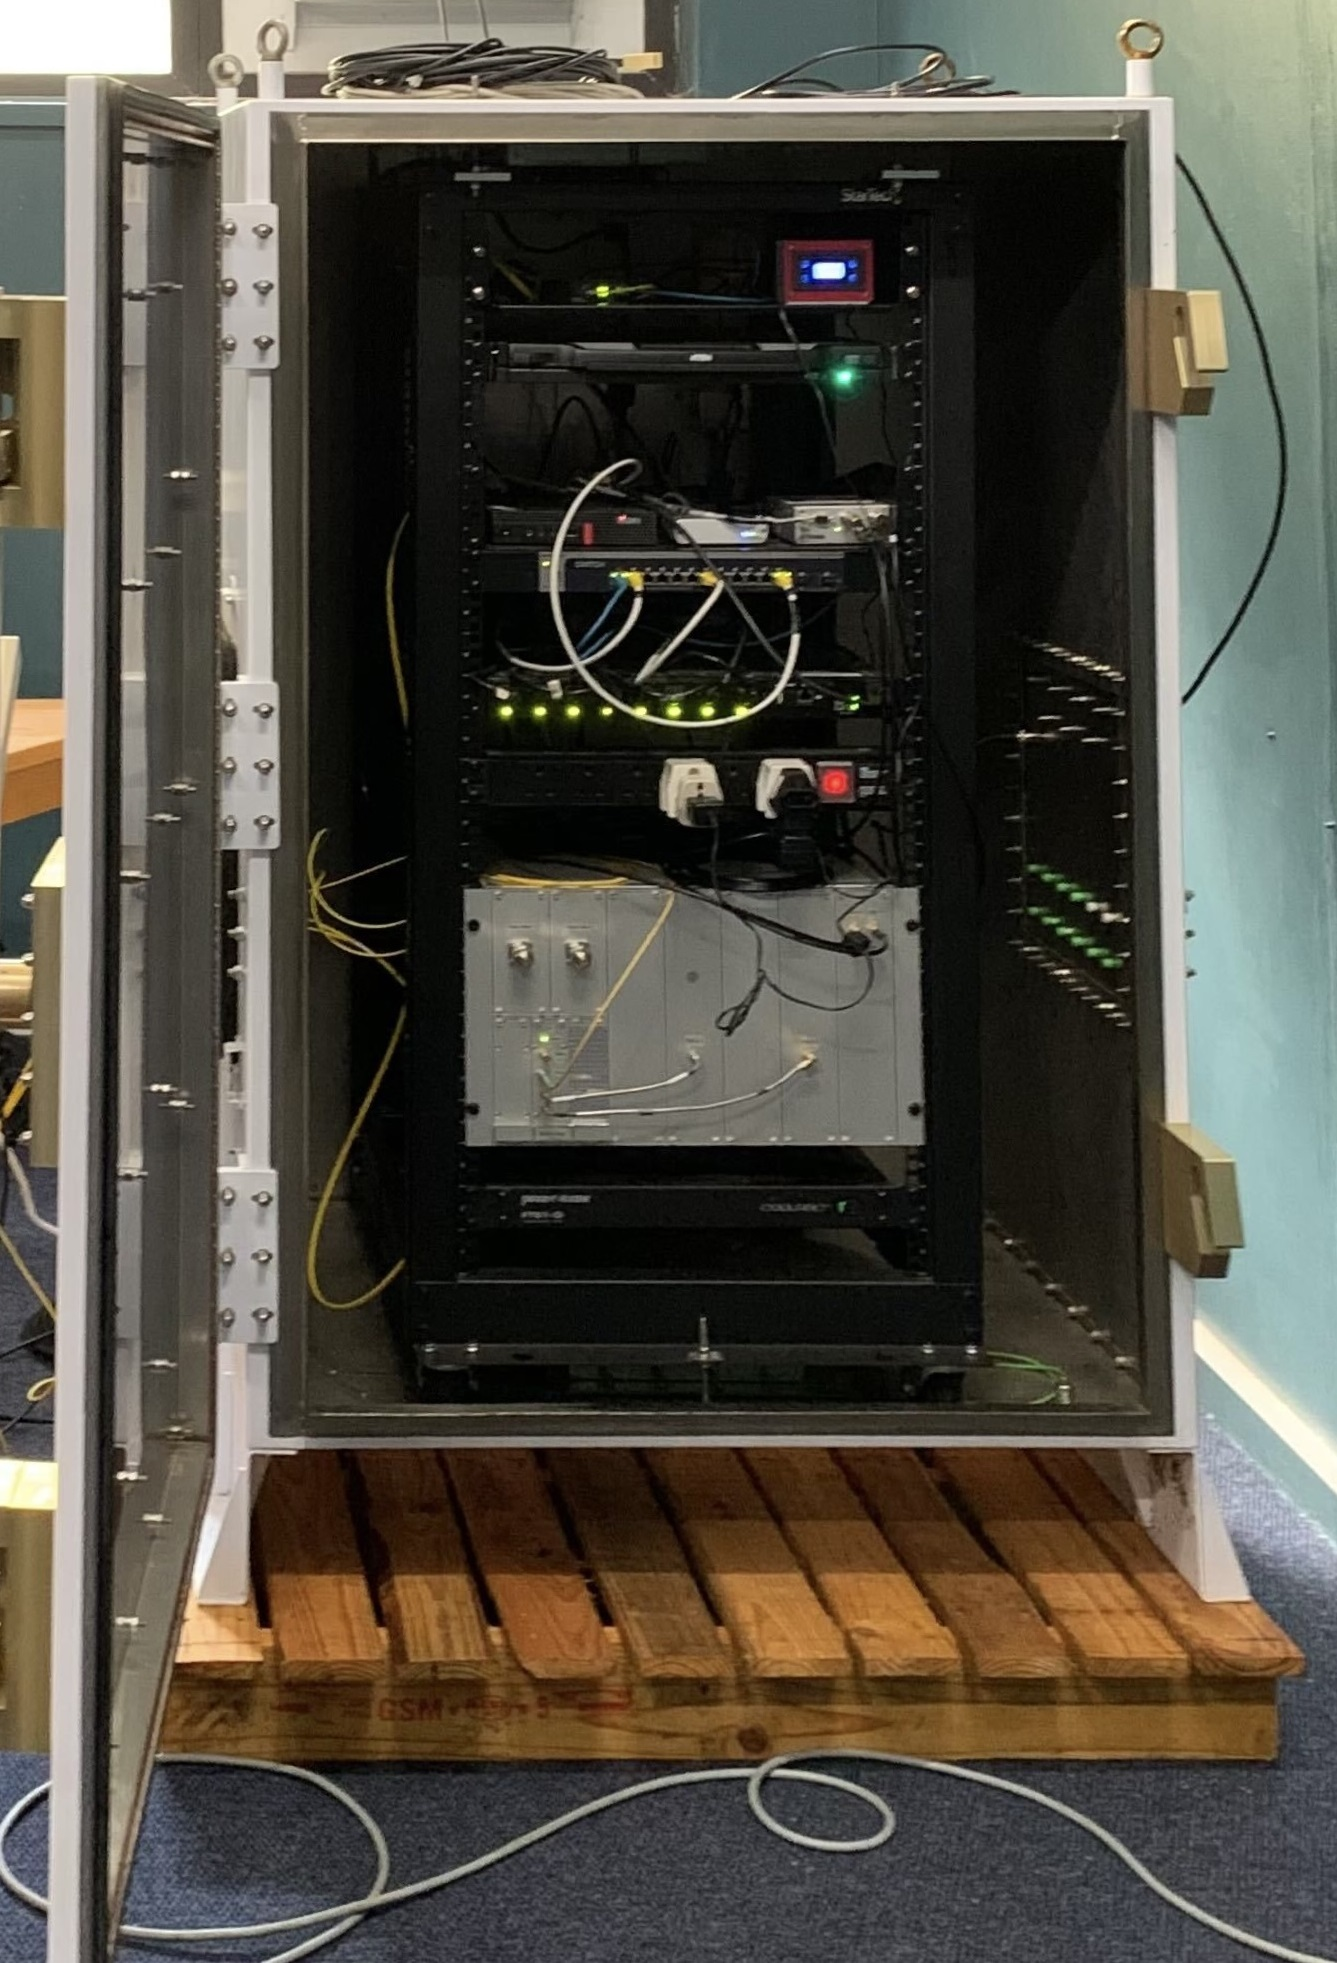
\includegraphics[width=\linewidth]{backend}
    \end{subfigure}
    \caption{A conceptual CAD rendering used as a reference for the REACH back-end RF-EMC enclosure is shown on the left exhibiting various custom assemblies for use in the South African Karoo such as ventilation paths and interference mitigation. The right image shows the completed receiver back-end rack housed inside the RF-EMC enclosure. Rack components such as the amplifier and spectrometer assembly (large silver module), ventilation and power distribution units can be seen.}
    \label{fig:backend}
\end{figure}

Within the RF-EMC enclosure are the various back-end modules mounted on a 36-inch rack\footnote{A StarTech 22U 36in Depth Enclosed Server Cabinet was used in Cambridge but not shipped for deployment.} also shown in \cref{fig:backend} which includes modules for additional signal amplification, conditioning and digitisation, the spectrometer for measurement of power spectral data, the back-end server and GPS system for remote communication and automation of the device, as well as power distribution and cooling units as detailed in this section. The back-end RF-EMC enclosure is accompanied by a smaller similar chamber to house various additional units such as a 7400 Wh SS202 Lithium Iron Phosphate battery made by Solar MD for overnight power storage from the solar panels or during periods of non-ideal weather. This smaller chamber is shown in \cref{fig:power_chamber} for reference but is not strictly a part of the receiver back-end.


% =========================================
\subsubsection{RF signal chain III: Amplifier \#2 and out-of-band injection}
The first device in the receiver back-end is our third stage of amplification with Amplifier \#2 (AMP2). Upon entering AMP2, the RFoF signal from the front-end is converted back into an RF signal by the optical receiver, again constructed with an FC/APC connection to a Polycom printed circuit board mounted to the AMP2 module. The next task of AMP2 is to continue filtering the signal using another Mini-Circuits XLF-42M+ 2-stage MMIC low-pass filter to block high-frequency out-of-band signals. To sharply filter signals outside the REACH observational band (above 170 MHz), a custom 11-order Cauer Chebyshev low-pass filter was designed using a series of five 1812SMS air core inductors made by Coilcraft as shown in the circuit diagram \cref{fig:amp2_schematic}. Following this, the signal is amplified using two more Mini-Circuits GALI-S66+ and PHA-13LN+ amplifiers, as used in AMP1, to achieve best dynamic range prior to the analogue-to-digital converter (ADC) within the iTPM spectrometer module. Low-loss 3 dB Mini-Circuits RCAT-03+ equalisation circuits are also used throughout AMP2 to flatten the passband to 2 dB. The final sub-component of AMP2 is a power splitter to output two equal signals from the module with one path going to the ADC/spectrometer unit and the duplicated signal available for additional devices such as another ADC or a power meter for remote monitoring as done with the HERA experiment.

Supplementary to AMP2 was an optional module for out-of-band continuous wave or filtered noise signal injection to condition the ADC. This unit was built to inject a constant power (adjustable through the inclusion of attenuators) at 10 MHz and is band limited to DC--20 MHz, strictly outside the REACH observational band as not to contaminate the measurement. An example of the injected out-of-band noise from this module is shown in \cref{fig:oob_cond}, though this feature was not used in the final deployed system as it provided no tangible improvements to the data as discussed in the THINGS THAT DIDNT WORK SECTION.
\begin{figure}
    \centering
    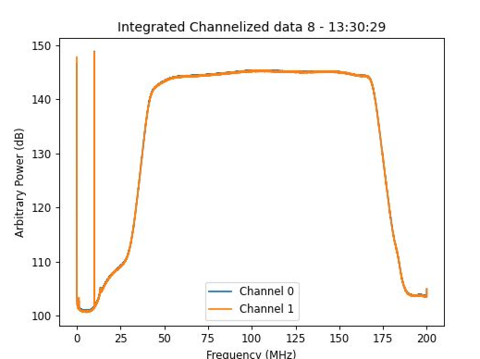
\includegraphics[scale=0.5]{oob_cond}
    \caption{A power spectral measurement of the ambient temperature $50 \Omega$ load with the out-of-band noise injection module activated. A constant power is injected at 10 MHz and can be used to assess the accuracy of the spectrometer reading as well as condition the ADC for low-power signals. Attenuators were used to prevent signals resonant to the 10 MHz injection from intercepting the in-band measurements. The spike at 0 MHz is an artefact of the spectrometer and receiver architecture and is not considered a hazard to the measurement.}
    \label{fig:oob_cond}
\end{figure}
The completed AMP2 and out-of-band injection unit are shown in \cref{fig:amp2} which represent the final components of the RF signal chain.
\begin{figure}
    \centering
    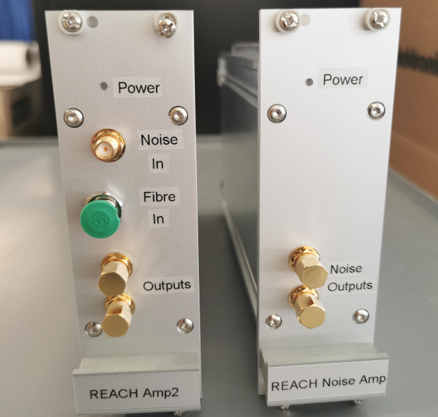
\includegraphics[scale=0.6]{amp2}
    \caption{The completed Amplifier \#2 (left) and out-of-band noise injection module (right) for inclusion in the receiver back-end. The ‘Fibre In’ port on AMP2 connects to the RFoF link from the front-end and the power splitter outputs identical signals to the ports labelled ‘Outputs’. The ‘Noise Output’ ports from the noise injection module would connect to the ‘Noise In’ port of AMP2 though this is not currently applied to measurements in the field.}
    \label{fig:amp2}
\end{figure}


% =========================================
\subsubsection{RF signal chain IV: Simulations}
Within the design process of the RF signal chain components; the LNA, AMP1 and AMP2, were various stages of optimisation and fine-tuning. Constituent elements within the LNA were first simulated then built and measured with the PNA-X as shown in \cref{fig:lna_sparams}. This data was then imported back into the simulation to further inform the development of the signal chain as a whole. Simulations were undertaken using the Keysight PathWave RF Synthesis software (formerly known as Genesys) with the in-program optimisation tool used to optimise filter design. Both linear analysis and the Keysight Spectrasys RF System Simulation software were also employed for RF budget simulations with other components simulated using Modelithics’ substrate scalable models. Also included in the simulations were measurements the AMP1 optical transmitter, AMP2 optical receiver and 100 metres of single-mode fibre, characterised by the VNA at different power levels and added to the simulation as a single block as shown in \cref{fig:chain_block_diag} which replicates the complete RF signal chain.
\begin{figure}
    \centering
    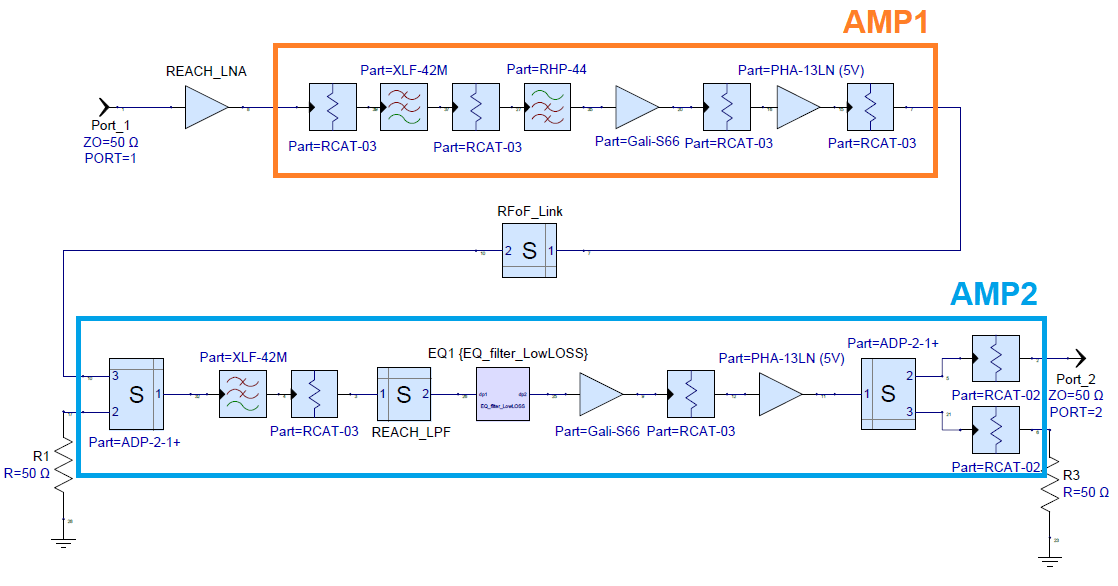
\includegraphics[width=\textwidth]{chain_block_diag}
    \caption{REACH RF system end-to-end block simulations made with the Keysight PathWave RF Synthesis software showing the LNA, AMP1, AMP2 as well as the RFoF link.}
    \label{fig:chain_block_diag}
\end{figure}
The results of the full RF signal chain simulations are shown in \cref{fig:chain_sim} where we highlight the flat noise figure of the network over the observational band.
\begin{figure}
    \centering
    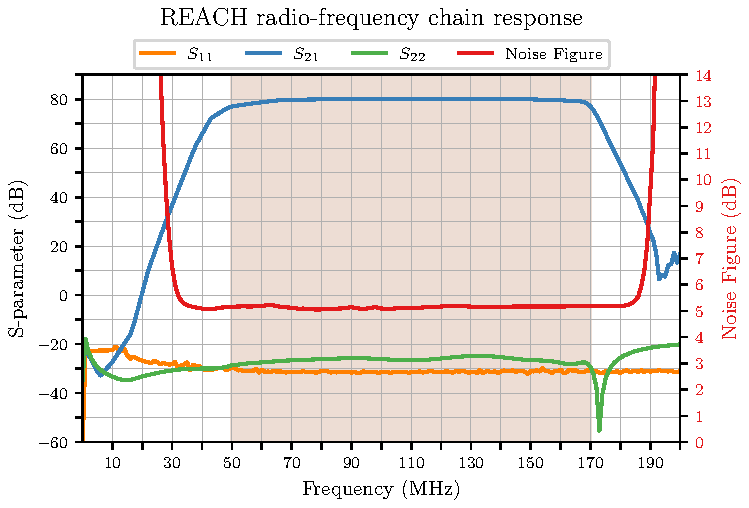
\includegraphics{chain_sim}
    \caption{Simulated radio-frequency response of the REACH end-to-end signal-chain as diagrammed in \cref{fig:chain_block_diag} which includes the LNA, AMP1, AMP2 and RFoF modules. VNA measurements of the LNA have been included in this simulation as well. The shaded region represents the REACH observation band where we see a flat noise figure throughout. Adapted from figure included in REACH NATURE PAPER.}
    \label{fig:chain_sim}
\end{figure}


% =========================================
\subsubsection{Spectrometer}
Following the amplification stages is the Sanitas EG \textit{italian} Tile Processor Module (iTPM) shown in \cref{fig:tpm} which serves as an analogue-to-digital converter (ADC) and a high-resolution ultra-wideband digital spectrometer.
\begin{figure}
    \centering
    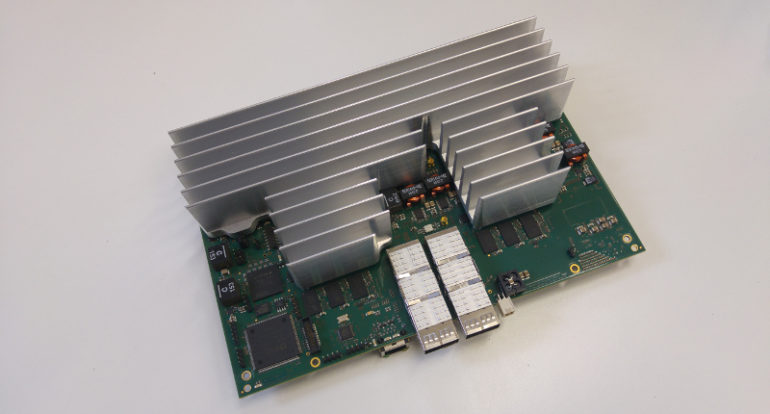
\includegraphics[scale=0.4]{tpm}
    \caption{The Sanitas EG italian Tile Processor Module for conversion of analogue signals to digital as well as spectral measurements.}
    \label{fig:tpm}
\end{figure}
This device was chosen for its development under the Square Kilometre Array experiment as part of the Low Frequency Aperture Array and has been used for verification of an SKA1 station as well as for back-end signal processing in other experiments \citep{itpm}. The iTPM's design targeting similar EoR signals granted easy reconfiguration for the REACH experiment through the reuse of auxiliary functions such as control, monitoring and data acquisition. Conversion of the incoming analogue signal to digital is undertaken using sixteen dual-channel Analog Devices 14-bit AD9680 ADCs allowing for multiple data streams from additional proposed antennas as detailed in the FUTURE WORK SECTION. At the time of deployment, two ADC channels were initialised as seen in the \cref{fig:oob_cond} legend for the two antennas expected to be built with the remaining ADC channels disabled to save power. Analogue signals are digitised at 400 MSPS using 16,384 channels at 12.2 kHz per channel. After conversion, spectral measurements are taken by two AMD XILINX UltraScale XCU40 field-programmable gate arrays (FPGAs) each customised to process a single digitised RF signal using a full floating-point fast Fourier transform (FFT), power integrator and polyphase filter bank incorporating 229,376 tap coefficients downloadable to the FPGA to allow the implementation of different weighting functions without recompiling the FPGA firmware. Spectra are accumulated over a number of FFT frames corresponding to an integration time of approximately one second which are then transmitted to a processing server via Ethernet connection where further accumulation can take place on the order of minutes. A typical spectrum obtained from a 20-minute integration on the $50 \Omega$ cold load is shown in \cref{fig:psd_cold}.
\begin{figure}
    \centering
    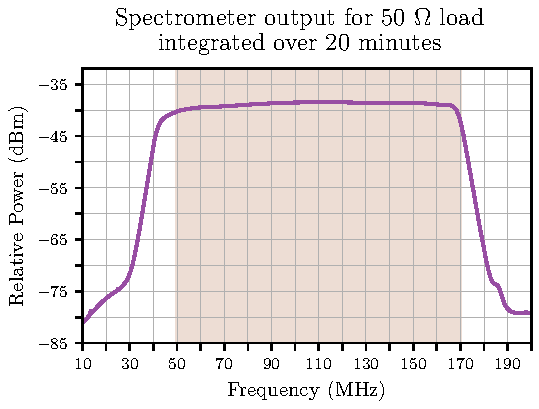
\includegraphics{psd_cold}
    \caption{A spectra taken by the iTPM of the ambient temperature $50 \Omega$ load integrated for 20 minutes using the finalised receiver system. A stable power measurement is seen within the REACH observational band (shaded region).}
    \label{fig:psd_cold}
\end{figure}
The 90 dB channel isolation of the spectrometer is expected to be useful for RFI excision. While on-site RFI measurements are still needed to confirm this, data from co-located experiments such as HERA suggest that the current channel isolation is adequate.


% =========================================
\subsubsection{Readout enclosure}
The readout system comprised of AMP2, the digitiser and spectrometer is housed in a custom-built 6U\footnote{housing height of six standard rack units approximately equal to 266.7 mm} metal enclosure as shown in \cref{fig:readout_enclosure}.
\begin{figure}
    \centering
    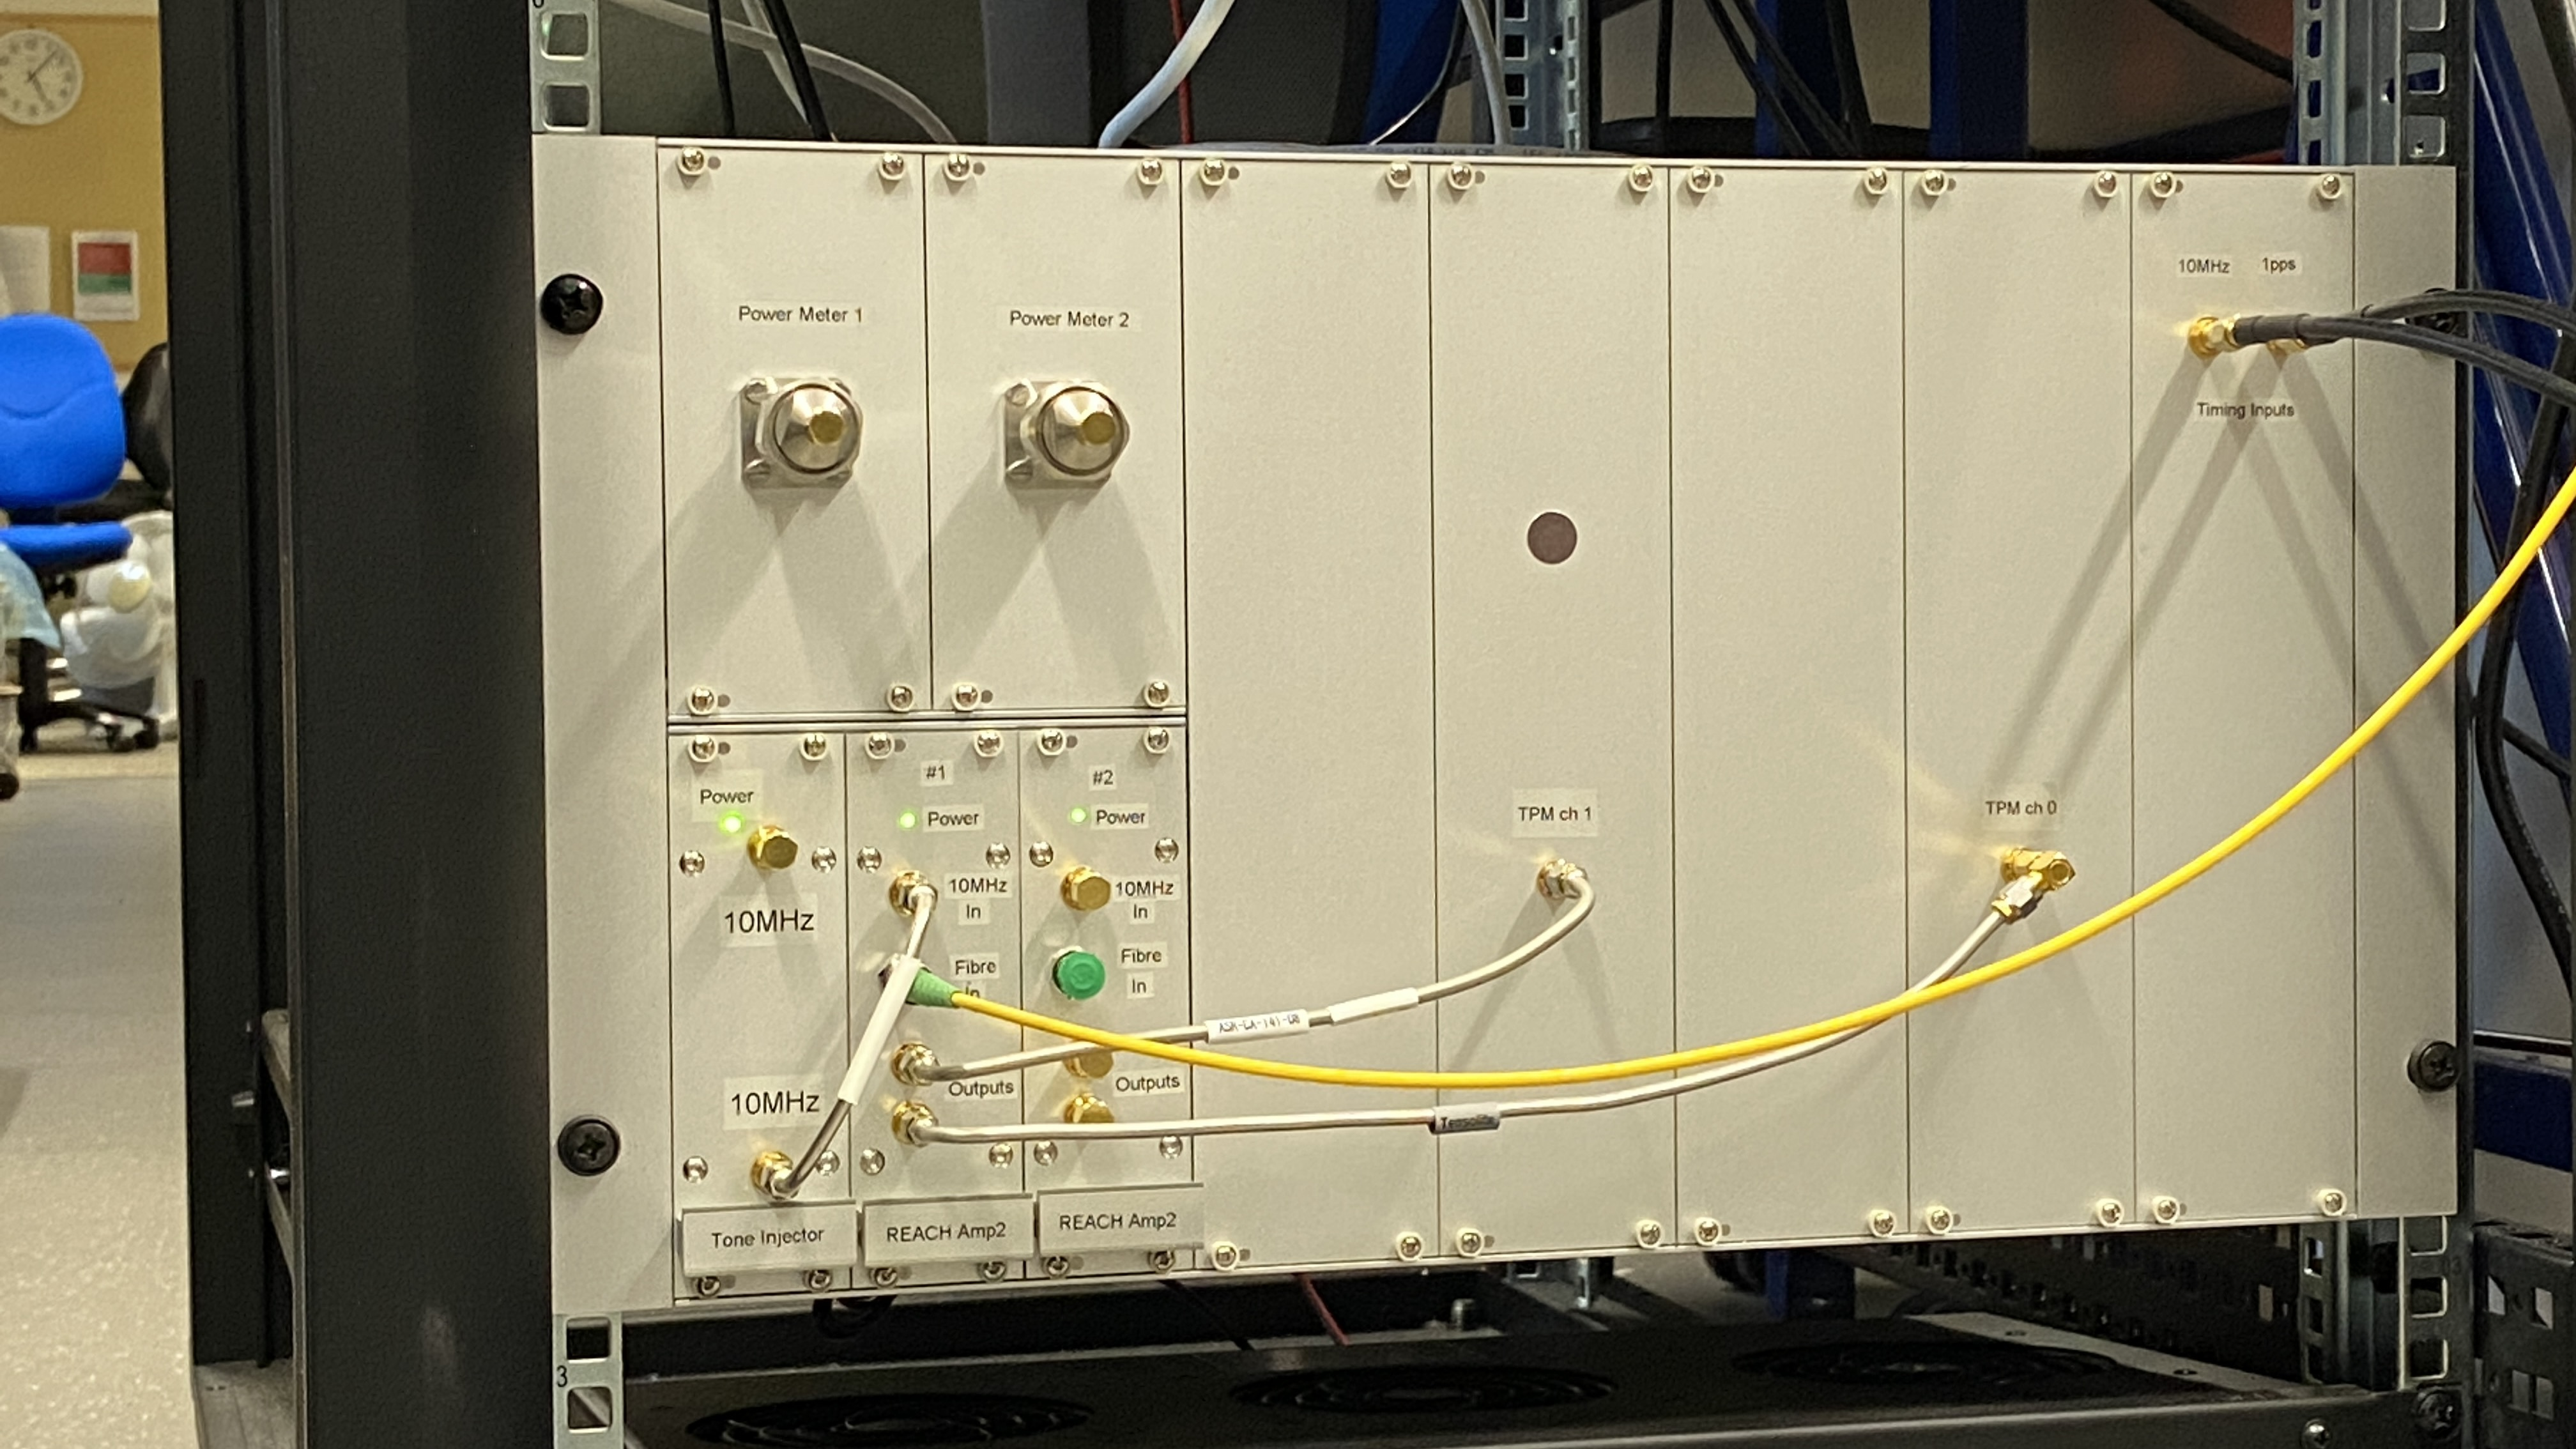
\includegraphics[width=0.7\textwidth]{readout_enclosure.jpeg}
    \caption{The readout enclosure housing the receiver components needed for digitisation and spectral measurements of radio-frequency signals.}
    \label{fig:readout_enclosure}
\end{figure}
Included in the readout enclosure are installations for two USB power meters to independently monitor absolute power levels in the field as previously detailed as well as slots for the out-of-band noise injection module and two independent Amplifier \#2 modules to accommodate two antennas in the field. Semi-rigid RG-405 connect the AMP2 outputs to iTPM channel inputs allocated individual panels seen in \cref{fig:readout_enclosure}. Within the enclosure is an off-the-shelf Peltier heat exchanger, fan and insulation to help regulate the temperature of the readout system, though the back-end components are subject to less scrutiny for operating temperature and output directly to the communication server via RJ45 cabling. Also seen on the front panelling are timing inputs to connect the iTPM to the GPS unit as detailed in the next subsection.


% =========================================
\subsubsection{GPS unit for TPM synchronisation}
Tile processor modules, such as the one used in our readout system, are comprised of a series of processing units referred to as ‘tiles’ which work in tandem to perform tasks efficiently. For precision applications, synchronisation among tiles is crucial for overall performance and a reference oscillator is needed to provide a common clock signal coordinating the timing of operations across different tiles. As we do not know the environmental effects of the deployment site on the iTPM’s internal oscillator a priori, we use an external Thunderbolt E GPS disciplined clock made by Trimble to ensure iTPM tiles operate in harmony. The Thunderbolt E links to a proprietary GPS antenna through a $75 \Omega$ Belden 1189A cable which allows the module to communicate with the global positioning system to generate a 10 MHz oscillation which is used as a reference to produce a 400 MHz clock to set the ADC sampling rate of 400 MSPS. The module then relays a pulse per second (PPS) signal to synchronise the ADCs to ensure coherence. The GPS disciplined clock was chosen over alternative atom-based frequency standardisation modules to ensure the reference clock accuracy, and in turn the sampling clock accuracy, is isolated from environmental effects, damage during transport, or interference generated by our own receiver components. This would in theory increase accuracy by limiting the propagation of delayed clock signals across tiles (known as skewing), and small variations in clock signal timings (known as jitter). Furthermore, a single reference should be used when using multiple TPMs, as may be the case in the future, to avoid slightly different sampling rates based on individual oscillators. Users of the receiver back-end should note that the 10 MHz GPS signal is independent from the 10 MHz out-of-band noise injection and are urged to be aware of the similarly-named labelling throughout the instrument. The Trimble Thunderbolt E as well as its GPS antenna are shown in \cref{fig:gps}.
\begin{figure}
    \centering
    \centering
    \begin{subfigure}{.3\textwidth}
        \centering
        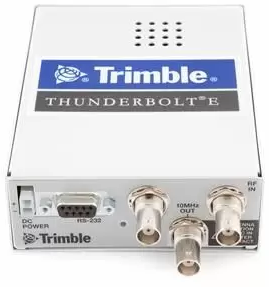
\includegraphics[width=\linewidth]{trimble}
    \end{subfigure}
    \hspace{.15\textwidth}
    \begin{subfigure}{.33\textwidth}
    \centering
        \includegraphics[width=\linewidth]{gps_ant}
    \end{subfigure}
    \caption{The Trimble clock discipline system consisting of the Thunderbolt E reference signal generator (left) and GPS antenna (right).}
    \label{fig:gps}
\end{figure}


% =========================================
\subsubsection{Server \& additional back-end units}
To permit communication between the instrument and users at Cambridge, a Lenovo M920q Tiny ThinkCentre with a ninthe generation Intel i7 core is included in the receiver back-end as a server. Xubuntu was chosen as the server operating system as the Xfce desktop environment uses fewer system resources in the field while retaining the flexibility and ease of use of Ubuntu\footnote{sorry Arch users…}. The ThinkCentre’s visual output connects to an ATEN CL6700 MW Single Rail LCD Console with built-in monitor keyboard and trackpad\footnote{Also referred to as a ‘KVM’ console for ‘Keyboard, Video \& Mouse’.} for in-person interaction with the machine during installation, triage and site trips when network connection may not be available.

USB links between the server and receiver components is achieved with a StarTech MODEL NUMBER 10-port USB hub with its primary function of receiving the USB over fibre signal from the front-end through the Icron 2244 USB Ranger’s optical-to-USB transducer. As detailed in \cref{sec:frontend}, this allows for the collection of reflection coefficient and temperature data as well as transmission of instructions to the microcontroller and front-end thermal management system. Additional ports on the StarTech USB hub connect the server to the back-end TEC controller for the Peltier device within the readout enclosure as well as a Penn Elcom FT01-Q module consisting of three rack-mounted fans for airflow and cooling within the receiver back-end. Finally, the USB hub connects the server to a Netgear ProSafe M4100-D12G Ethernet managed switch for control of further components via RJ45 connection. Connected to the Ethernet switch is the readout system output, permitting the collection of spectral data from the iTPM as well as connection to a Tripp Lite PDUMH15HVNET Ethernet controlled power distribution unit allowing users to toggle power for individual devices throughout the receiver back-end. The Ethernet switch will also be connected to the satellite uplink intended to be installed after the receiver back-end but not finalised at the time of writing. A second PDU was included in the deployed back-end but is not used. Tables specifying the connections of the USB hub, Ethernet switch and back-end PDU are given in \cref{tab:usb_hub}, \cref{tab:eth_switch} and \cref{tab:backend_pdu} respectively for reference.


% =========================================
\subsubsection{Completed receiver back-end unit}
The receiver back-end was also finished in December 2022 and is shown in \cref{fig:backend_complete}.
\begin{figure}
    \centering
    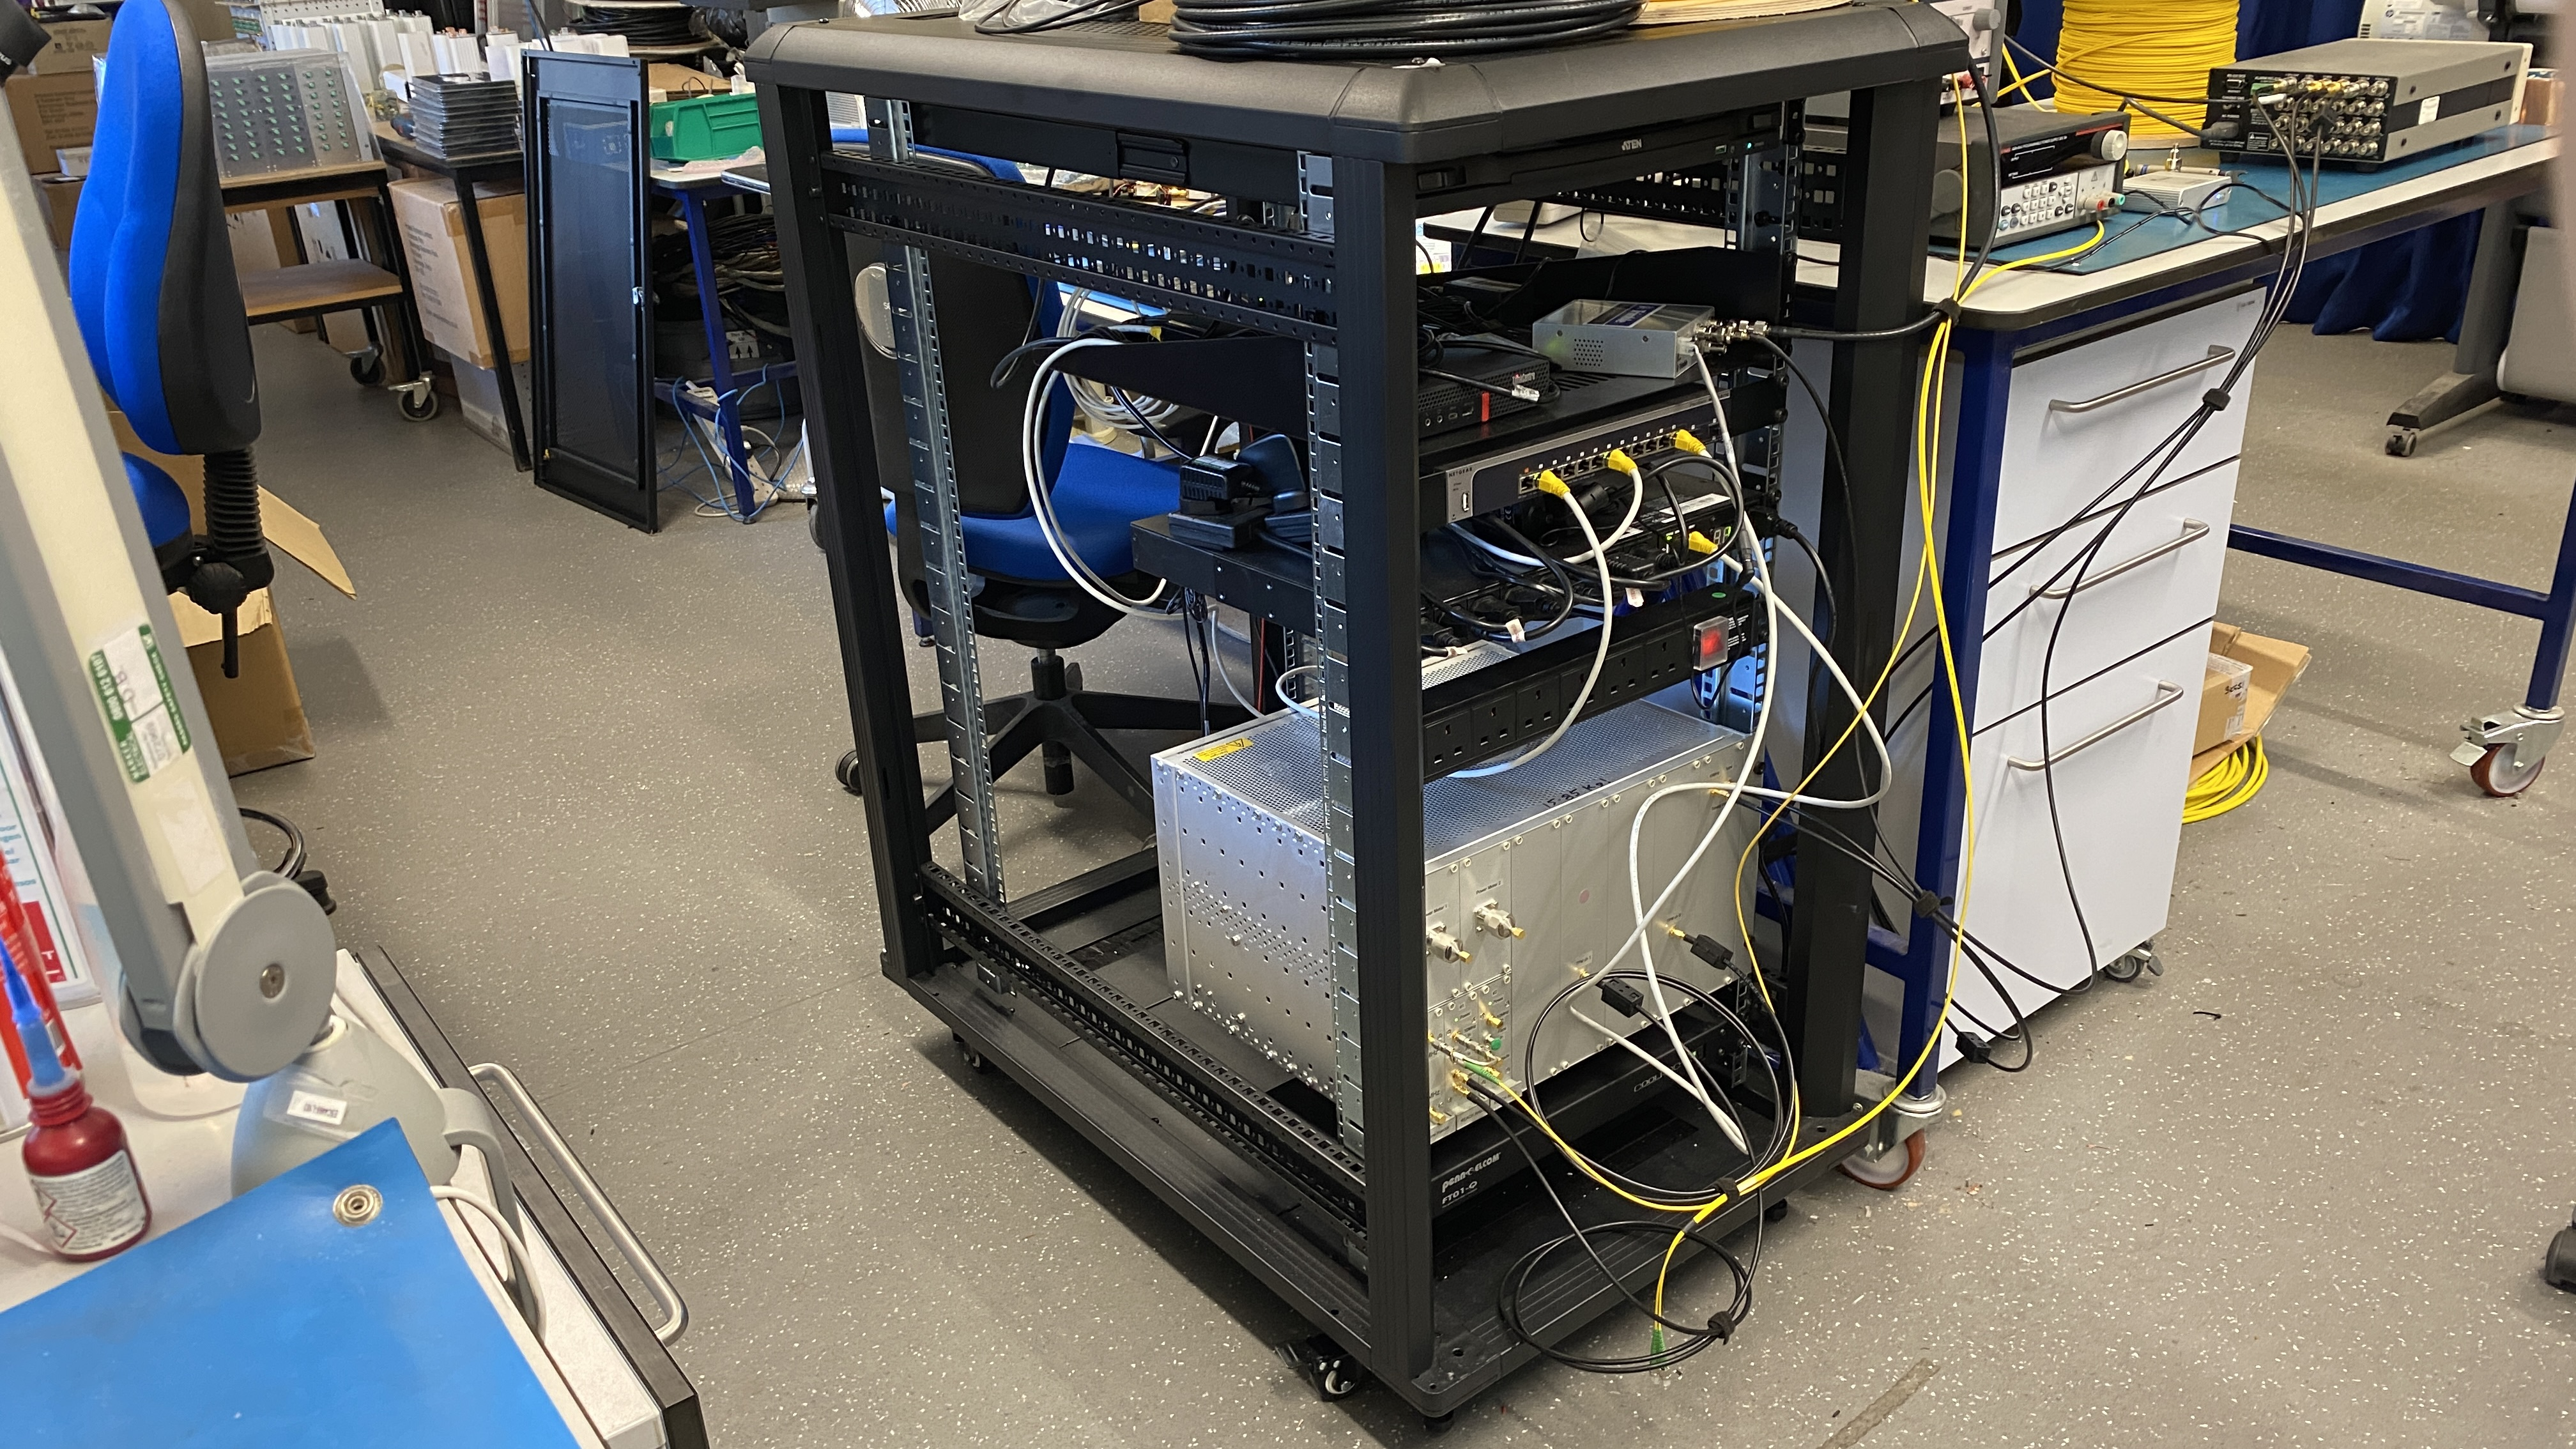
\includegraphics[width=.7\textwidth]{backend_complete}
    \caption{The completed receiver back-end installed in the 36-inch rack in Cambridge (minus the RF-EMC enclosure). The custom readout system weighs in at 15.89 kilograms and is central to the experiment's data acquisition. The Ethernet switch and power distribution units can be seen and are controlled by the Lenovo server. This unit would be common to any additional antennas deployed to the field and is generally less sensitive to environmental effects on site.}
    \label{fig:backend_complete}
\end{figure}
The completed build was too large to be shipped practically and was disassembled into its constituent submodules before being sent to South Africa in February 2023 and reconstructed using a different standardised rack. This finalised construction is intended to serve as a central node for the REACH experiment including any further antennas to be  deployed on site. As much of the receiver back-end consists of off-the-shelf components, we expect serviceability and part replacement to be more straightforward than the front-end. A diagram indicating the back-end submodules is shown in \cref{fig:backend_diag}.
\begin{figure}
    \centering
    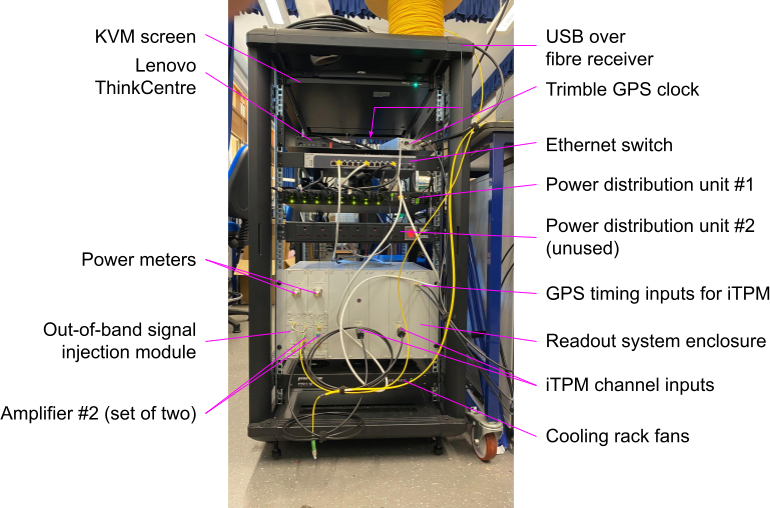
\includegraphics[width=\textwidth]{backend_components}
    \caption{A diagram specifying the placement of the various back-end components for the completed unit in December 2023.}
    \label{fig:backend_diag}
\end{figure}


% =========================================
\subsection{Automation}
The nearest settlement to the REACH deployment site in the Karoo Radio Reserve is Carnarvon, about 90 kilometres away and about seven hour’s drive from the central international airport in Cape Town. Such isolation made the development of a fully autonomous instrument a necessity and procedures were developed to facilitate remote access and communication with the device. In our procedure, the receiver front-end(s) and back-end are controlled and monitored by our management software running on the Lenovo processing server which oversees operation of the instrument such as the configuration of hardware components, data management and directing subroutines. Within our management software, a variety of different communication protocols are used. The Python FPGA Board Interface Layer (PyFABIL) is used to interact with the iTPM while the Standard Commands for Programmable Instruments (SCPI) protocol is used to contact the VNA. Proprietary USB protocols in a Python wrapper are used by the TC-08 temperature sensor with the TEC needing an additional proprietary Windows-based Application Programming Interface which entails a virtual machine running in our Linux desktop environment. Signal path configuration through the microcontroller unit is assigned to Teensy ports accessed through a command line serial interface. A crib sheet useful for the development of automated procedures such as an observation schedule is shown in \cref{fig:controller_pinout} which details the specific devices contactable through individual microcontroller ports.
\begin{figure}
    \centering
    \includegraphics{controller_pinout}
    \caption{A reference sheet listing the front-end component assignments to the Teensy input/output ports for use in receiver automation. Individual switch positions, power supplies and components can be seen facilitating the creation of new automated routines and on-the-fly system interaction via command line interface. MS‘N’--‘P’ refers to mechanical RF switch number N, port P. ‘MTS’ is the mechanical transfer switch. ‘TEC’ is the thermo-electric cooler module.}
    \label{fig:controller_pinout}
\end{figure}

Both the calibration and observation procedures are managed by a YAML configured scheduler allowing a remote operator to specify a sequential list of operations including switch toggling, reflection coefficient or spectral measurement, the VNA calibration and hardware initialisation among other low-level commands for debugging purposes. General prescriptions are provided for the two main operations, the first of which is calibration. During calibration, the instrument is instructed to first calibrate the VNA through measurement of the S-O-L standards as detailed in \cref{sec:frontend}. Following this, a measurement of the $50 \Omega$ test load is compared to a saved file from the PNA-X on a frequency-by-frequency basis. If the VNA measurements are within a user-defined tolerance (usually 5\%), the instrument proceeds with receiver calibration measurements; S\textsubscript{11}, spectra and temperatures of the calibration sources along with an S\textsubscript{11} measurement of the LNA. This data is fed into the calibration algorithm to generate calibration coefficients which are verified through comparison with a benchmark set of coefficients to within a user-defined tolerance (e.g. previous calibration coefficients to within 5\%).

Following this is the second primary mode of operation; observation. During observation, power spectral measurements of the sky, reference load and reference noise source as part of the Dicke cycle are performed by the YAML-configured schedule started by a local sidereal time (LST) trigger. Additional measurements of the test load are taken to support ad hoc debugging procedures after which RFI in the data is flagged by a separate algorithm. Calibration coefficients derived in the calibration routine are then applied to the data before being set for data processing. A flowchart depicting the general steps of instrument operation is shown in \cref{fig:obs_flowchart}.
\begin{figure}
    \centering
    \includegraphics[width=\columnwidth]{updated_reach_obs_loop}
    \caption{Typical REACH calibration and observation loop including calibration of the VNA and receiver as well as data acquisition, checks and processing such as RFI flagging. Various stages are verified via algorithm before proceeding to the next process.}
    \label{fig:obs_flowchart}
\end{figure}

The receiver back-end transmits integrated spectra as Streaming Protocol for Exchanging Astronomical Data User Datagram Protocol (SPEAD UDP) packets over a 1 GbE network to be received by the associated spectrometer module. A software monitoring daemon collects temperature and power information every minute which is stored in a metric database which are included as metadata with calibration and observation data to inform the calibration procedure. The generated data is then stored as an HDF5 file which includes spectra and reflection coefficients with associated timestamps along with temperature sensor readings. The HDF5 files are self-describing, containing all the information required for future processing without having to refer to observation schedules or similar documentation. The HDF5 files then are transferred off-site to a centralised storage system through a satellite network link installed on-site. An plot of power spectral data taken remotely from Stellenbosch University in South Africa is shown in \cref{fig:remote_data}.
\begin{figure}
    \centering
    \includegraphics[scale=0.6]{remote_data}
    \caption{Passband measurements of several calibration sources taken remotely through an automated procedure. The spectral data shows a clean frequency response with small RFI spikes at lower frequencies which will need to be procees by the separate RFI flagger.}
    \label{fig:remote_data}
\end{figure}


% =========================================
\subsection{Deployment}
Throughout 2022, the deployment site in South Africa was prepared while receiver development took place. Ditches were dug for support posts to be placed for the raised ground plane mesh suspended by guide wires. Due to natural land slope on site, the ground plane was erected between 1 metre and 1.2 metres above ground level to maintain a level construction. Support structures were built and the antenna was then installed as shown in \cref{fig:ground_plane}.
\begin{figure}
    \centering
    \includegraphics[width=\textwidth]{ground_plane}
    \caption{The REACH dipole antenna on the raised wire mesh ground plane. Support posts of heights varying 20 cm were raised to provide a level ground plane in contrast to the sloped land underneath.}
    \label{fig:ground_plane}
\end{figure}
Upon being shipped from Cambridge, the receiver front and back-ends underwent strict electromagnetic compatibility (EMC) testing at the Karoo radio reserve under the same level of scrutiny as co-located experiments such as HERA. After a final round of testing by the REACH team, the receiver was transported to the deployment site in August 2023 where the back-end components were installed as shown in \cref{fig:deploy_backend}.
\begin{figure}
    \centering
    \includegraphics[width=.8\textwidth]{deploy_backend.jpg}
    \caption{The receiver back-end and support enclosure underneath the solar panel installation at the deployment site.}
    \label{fig:deploy_backend}
\end{figure}

It was understood that at some time between shipment from Cambridge and deployment in the field that both the front-end TEC Peltier device as well as satellite infrastructure had been damaged and no longer functioned. The front-end has been sent back to Stellenbosch University to investigate the fault. Despite this, in-field sky spectra was taken, a screenshot of which can be seen in \cref{fig:onsite_data}.
\begin{figure}
    \centering
    \includegraphics[scale=0.4]{onsite_data}
    \caption{A screenshot from the REACH's first light showing on-site sky data collected by the dipole and taken directly from the back-end KVM console using a mobile phone. The themoelectric cooling unit damaged during transport was not running during this data acquisition. The spectra seen are uncalibrated and underwent no data processing which causes the spectra to deviate from the characteristic power-law form expected of the foregrounds at low and high frequencies. The shaded region is the FM radio broadcast band for South Africa (87.5 -- 108 MHz).}
    \label{fig:onsite_data}
\end{figure}
As a disclosure, it should be noted that this in-field data was left on a USB flash drive on site and here, a snapshot from the KVM screen taken with a phone camera is used. The image has been enhanced using Microsoft Lens and the GNU Image Manipulation Program (GIMP). While the spectra shown in \cref{fig:onsite_data} is raw, uncalibrated data that hasn't gone through any processing, some important details can be derived from the plot. Firstly, spectra from the antenna is generally higher than the calibrator spectra which serves as a sanity check. Secondly, more than half of the RFI spikes seen in the antenna spectra lie within the FM radio broadcast band for South Africa (87.5 -- 108 MHz) as highlighted in purple, confirming that our apparatus is indeed receiving radio-frequency signals. Further verification can be undertaken by cross checking the precise broadcast frequencies of local radio stations. Finally, we can also see that the antenna spectra peaks at low frequencies and decays off, approximating the power law shape of galactic synchrotron emission expected from sky measurements at these frequencies COMPARE WITH POWER LAW SKY MEASUREMENT IN EDGES RESULT. We therefore conclude that these spectra are encouraging as an initial proof-of-concept measurement.

Furthermore, it has also been seen that, due to the changing weather conditions on site, the $20 \times 20$ metre ground plane\footnote{with 6 metre serrations} sags due to insufficient support. Provisional supports were made with scrap wood as seen in \cref{fig:ground_plane} while a more permanent method of support is currently deployed. With the approximate completion of the ground plane, installation of the dipole antenna, solar panels and receiver back-end, the REACH site can be seen through satellite imaging at the latitude-longitude coordinates 30\textdegree50'19.4"S 21\textdegree22'29.8"E as shown in \cref{fig:sat_image}.
\begin{figure}
    \centering
    \includegraphics[width=\textwidth]{sat_image}
    \caption{A satellite image from Google Earth showing the REACH deployment site. The 20 metre wide ground plane can be seen with the antenna installed at its centre. To the upper right of the ground plane is the back-end node covered by the solar panel installation. The lower left shows two vehicles and a tent with a dirt road exiting the site on the left along the ground plane.}
    \label{fig:sat_image}
\end{figure}
